%% LaTeX2e class for student theses
%% sections/content.tex
%% 
%% Karlsruhe Institute of Technology
%% Institute for Program Structures and Data Organization
%% Chair for Software Design and Quality (SDQ)
%%
%% Dr.-Ing. Erik Burger
%% burger@kit.edu
%%
%% Version 1.1, 2014-11-21


\chapter{Theoretical Framework}
\label{chap:chap_theo}

\newacronym{cfd}{CFD}{computational fluid dynamics}
\newacronym{smb}{SMB}{simulated moving bed chromatography}
\newacronym{hgms}{HGMS}{high gradient magnetic separation}
\newacronym{pde}{PDE}{partial differential equation}
\newacronym{fem}{FEM}{finite element method}
\newacronym{bdf}{BDF}{backward differentiation formula}

In the first part of this chapter the fundamentals of magnetism are described (see Section\,\ref{sec:Fund_mag}). In Section\,\ref{sec:Mag_sep} the basic principles of the forces acting in a magnetic separation process are explained, as well as the acting physical forces. In the second part of this chapter the fundamentals of \gls{cfd} are discussed (see Section\,\ref{sec:CFD}) and in Section\,\ref{sec:smb} a brief overview on \gls{smb} is given.  

\section{Fundamentals of magnetism}
\label{sec:Fund_mag}
The focus of this thesis was to establish a size separation process for nanoparticles by using magnetic separation technologies. The concept of magnetic separation is based on the properties of magnetic fields and magnetic materials. Therefore the following sections give an overview of the fundamental equations and material properties related to magnetism. Magnetism is a physical phenomenon produced by the motion of electric charges, which results in attractive and repulsive forces between objects \cite{stevenson2010oxford}. Electric currents and the magnetic moments of elementary particles are the origin of magnetic fields, which generate these forces. Sections \ref{subsec:Maxwell}, \ref{subsec:const_rel} and \ref{subsec:Mag_pot} give an overview of the basic electromagnetic equations describing those fields, while in Section\,\ref{subsec:Mag_mat} the magnetic properties of materials are discussed.

\subsection{Maxwell's equations}
\label{subsec:Maxwell}
%%%%%%%%%Quellen einfügen%%%%%%%%%%%%%%%%%%%%%%%%%%%%%%%%%%%%%%%%%%% \cite{kallenbach2018elektromagnete}
The correlation between magnetic and electric fields, as well as the relation of those fields to electrical charges and currents, are described by  Maxwell’s equations. In combination with the Lorentz force law these equations describe all classical electromagnetic phenomena \cite{meschede2015gerthsen}. The macroscopic Maxwell equations (see Equations\,ref{eq:Faraday}, \ref{eq:Ampere}, \ref{eq:Gauss_elec} and \ref{eq:Gauss_mag}) for general time-varying fields in the differential form are as follows \cite{monk2003finite}: 

\begin{equation}
\label{eq:Faraday}
\centering
\nabla\times\boldsymbol{E} = -\frac{\partial\boldsymbol{B}}{\partial t}
\end{equation}

\begin{equation}
\label{eq:Ampere}
\centering
\nabla\times\boldsymbol{H} = \boldsymbol{J} + \frac{\partial\boldsymbol{D}}{\partial t}
\end{equation}

\begin{equation}
\label{eq:Gauss_elec}
\centering
\nabla\cdotp\boldsymbol{D} = \rho 
\end{equation}

\begin{equation}
\label{eq:Gauss_mag}
\centering
\nabla\cdotp\boldsymbol{B} = 0
\end{equation}

where the used fundamental electromagnetic quantities are the electric field intensity $\boldsymbol{E}$ in V/m, the magnetic flux density $\boldsymbol{B}$ in T, the magnetic field intensity $\boldsymbol{H}$ in A/m, the electric current density $\boldsymbol{J}$ in A/m\textsuperscript{2}, the electric flux density $\boldsymbol{D}$ in C/m\textsuperscript{2} and the electric charge density $\rho$ in C/m\textsuperscript{3} \cite{meschede2015gerthsen,monk2003finite}. $\nabla\times$ stands for the curl operator which is a measure of the rotation of a vector field, while $\nabla\cdotp$ denotes the divergence of a field. Equation\,\ref{eq:Faraday}, also known as Faraday's law, describes how a time varying magnetic field induces a spatially varying electric field, while Equation\,\ref{eq:Ampere}, which is referred to as Ampere's law, states that magnetic fields are generated by either electric currents or time varying electric fields. Together they describe the propagation of electromagnetic waves. Equation\,\ref{eq:Gauss_elec} and \ref{eq:Gauss_mag} are called Gauss's law and Gauss's law of magnetism respectively. Equation\,\ref{eq:Gauss_elec} gives the effect of the charge density on the electric field. It states that the electric flux through any hypothetical closed surface is proportional to the net electric charge enclosed by this surface, which becomes obvious in its integral form. Gauss's law of magnetism states that, contrary to electric charges, magnetic monopoles do not exist and that $\boldsymbol{B}$ is always a solenoidal vector field. Instead, a magnetic field is induced by magnetic dipoles. Because of the relationship of $\boldsymbol{B}$ and $\boldsymbol{H}$ (see Equation\,\ref{eq:B_vac}) the divergence of the magnetic field intensity is also zero \cite{monk2003finite,kallenbach2018elektromagnete}.
The combination of Gauss' and Ampere's law results in the continuity equation (see Equation\,\ref{eq:Konti_Mag}) which specifies the conservation of charge. It states that the net quantity of charges is always conserved \cite{monk2003finite,meschede2015gerthsen,schwab2013begriffswelt}.   

\begin{equation}
\label{eq:Konti_Mag}
\centering
\nabla\cdotp\boldsymbol{J} = -\frac{\partial\rho}{\partial t}
\end{equation}

For static fields, i.e. no variation of the field quantities with time, the Equations \ref{eq:Faraday}, \ref{eq:Ampere} and \ref{eq:Konti_Mag} are reduced to:

\begin{equation}
\label{eq:Faraday_stat}
\centering
\nabla\times\boldsymbol{E} = 0
\end{equation}

\begin{equation}
\label{eq:Ampere_stat}
\centering
\nabla\times\boldsymbol{H} = \boldsymbol{J} 
\end{equation}

\begin{equation}
\label{eq:Konti_Mag_stat}
\centering
\nabla\cdotp\boldsymbol{J} = 0
\end{equation}

\subsection{Constitutive relations}
\label{subsec:const_rel}

In order to apply Maxwell's macroscopic equations they must be augmented with two constitutive relations. The constitutive relations describe the relationship between $\boldsymbol{D}$ and $\boldsymbol{E}$ as well as between $\boldsymbol{B}$ and $\boldsymbol{H}$ depending on the macroscopic properties of the medium. The constitutive relations in empty space can be written as Equations\,\ref{eq:disp_const_rel} and \ref{eq:B_vac}. 

\begin{equation}
\label{eq:disp_const_rel}
\centering
\boldsymbol{D} = \varepsilon_{0}\boldsymbol{E} 
\end{equation}

\begin{equation}
\label{eq:B_vac}
\centering
\boldsymbol{B} = \mu_{0}\boldsymbol{H}
\end{equation}

with the vacuum permittivity $\varepsilon_{0}$ which takes a value of 8.854$\cdotp$10\textsuperscript{-12}\,F/m and the vacuum permeability $\mu_{0}$ with a value of 4$\pi\cdotp$10\textsuperscript{-7} H/m \cite{monk2003finite,kallenbach2018elektromagnete}. For linear materials, which are characterized by a linear relation between the magnetization and the magnetic field intensity as shown in Equation\,ref{eq:chi}, the relationship between $\boldsymbol{B}$ and $\boldsymbol{H}$ is described by Equation\,\ref{eq:B_tot}. A similar relationship can be formulated for the electric field (see Equation\,\ref{eq:D_tot}).    

\begin{equation}
\label{eq:B_tot}
\centering
\boldsymbol{B} = \mu_{0}\mu_{r}\boldsymbol{H}
\end{equation}

\begin{equation}
\label{eq:D_tot}
\centering
\boldsymbol{D} = \varepsilon_{0}\varepsilon_{r}\boldsymbol{E}
\end{equation}

Here $\mu_{r}$ indicates the relative permeability of the medium, while $\varepsilon_{r}$ stands for the relative permittivity of the material. $\mu_{r}$ is a measure of the permeability $\mu$ of a material relative to that of vacuum (see Equation\,\ref{eq:mu_r}).
\begin{equation}
\label{eq:mu_r}
\centering
\mu_{r} = \frac{\mu}{\mu_{0}}
\end{equation}

 Materials with $\mu_{r}$ larger than one are called paramagnetic, while materials with a value of $\mu_{r}$ less than one are referred to as diamagnetic \cite{svoboda2004magnetic}. In contrast, ferromagnetic materials exhibit a hysteresis function. For a more detailed description of the material properties see Section\,\ref{subsec:Mag_mat}. The magnetic flux density is also influenced by the magnetization $\boldsymbol{M}$ of the material as shown below \cite{ichimura1989maxwell}: 

\begin{equation}
\label{eq:Mag}
\centering
\boldsymbol{B} = \mu_{0}(\boldsymbol{H} + \boldsymbol{M})
\end{equation}

For linear materials there is a directly proportional relationship between the magnetization and the magnetic field intensity with the specific/mass magnetic susceptibility $\chi$.  

\begin{equation}
\label{eq:chi}
\centering
\boldsymbol{M} = \chi\boldsymbol{H}
\end{equation}

Materials with positive values of $\chi$ are paramagnetic, whereas materials with negative values of $\chi$ are called diamagnetic. For ferromagnetic materials $\chi$ is dependent on the previous magnetization of the medium as well as the particle size and shape \cite{michalowsky2006magnettechnik}. The magnetic susceptibility is also related to the relative permeability (see Equation\,\ref{eq:chi_2}).

\begin{equation}
\label{eq:chi_2}
\centering
\chi = \mu_{r}-1
\end{equation}

For some materials a non-linear relationship between $\boldsymbol{B}$ and $\boldsymbol{H}$ can be found as shown in Equation\,\ref{eq:nonlin_B}.

\begin{equation}
\label{eq:nonlin_B}
\centering
\boldsymbol{B} = f(\vert\boldsymbol{H}\vert)
\end{equation}

\subsection{Magnetic vector potential}
\label{subsec:Mag_pot}
A solenoidal vector field can always be written as the curl of a different vector field. Consequently $\boldsymbol{B}$ can also be formulated as the curl of the magnetic vector potential $\boldsymbol{A}$. The magnetic vector potential $\boldsymbol{A}$ results from Gauss' law of magnetism (see Equation\,\ref{eq:Gauss_mag}). For magnetostatics $\boldsymbol{A}$ in Vs/m is related to $\boldsymbol{B}$ by the following Equation\,\ref{eq:Pot_A}.  

\begin{equation}
\label{eq:Pot_A}
\centering
\boldsymbol{B} = \nabla\times\boldsymbol{A}
\end{equation}

As a vector field can only be fully specified by its divergence and its curl $\nabla\cdotp\boldsymbol{A}$ has to be defined. By choosing $\nabla\cdotp\boldsymbol{A}$ the magentic vector potential is defined completely. In magnetostatics the gauge condition $\nabla\cdotp\boldsymbol{A}$ = 0 is applied \cite{schwab2013begriffswelt}.   

\subsection{Magnetic properties of materials}
\label{subsec:Mag_mat}

%%%%%%%%%Quellen einfügen%%%%%%%%%%%%%%%%%%%%%%%%%%%%%%%%%%%%%%%%%%%%%%%%%%

%Figure of permeability curves
%saturation is most clearly seen in the magnetization curve (also called BH curve %or hysteresis curve) of a substance, as a bending to the right of the curve (see %graph at right). As the H field increases, the B field approaches a maximum value %asymptotically, the saturation level for the substance.

For the separation of magnetic materials the differences in their magnetic behaviour is crucial, therefore a short overview of the different types of magnetic properties is given below. The origin of magnetism lies in the orbital and spin motions of electrons, therefore all materials are magnetic and show a magnetic response. The magnetic moments of the nuclei of the atoms are negligible. Usually,  the magnetic moments of the electrons within a material cancel each other out. When a material is placed in a magnetic field however the magnetic moments align. This effect is called magnetization. The main difference between different types of materials is the different alignment of the magnetic moments. According to their magnetic properties, materials can be divided into three main classes: diamagnetic, paramagnetic and ferromagnetic. In addition antiferromagnetic and ferrimagnetic materials can be defined. The different groups are listed in Table\,\ref{table:mag_material} distinguished by their material specific values of the relative permeability and the magnetic susceptibility. 

\begin{table}[H]
\centering
\caption{Classification of magnetic materials}
\label{table:mag_material}
\begin{tabular}{lll}\hline
class & relative permeability & magnetic susceptibility \\
\hline\hline
diamagnetic & $\mu_{r}<1$ & $\chi<0$ \\
paramagnetic & $\mu_{r}>1$ & $\chi>0$ \\
ferromagnetic & $\mu_{r}\gg1$ &  \\
\hline
\end{tabular}
\end{table}

Diamagnetism occurs in all matter, for para- and ferromagentic materials however this effect is negligible and will be masked by the other magnetic properties of the medium, consequently only materials with no other overlaying magnetic properties are alloted to the diamagnetic class. In the presence of a magnetic field the orbital magnetic moments aligned in the opposite direction of the external field are increased, while the moments aligned parallel to the external field are decreased. Therefore diamagnetic materials are repelled by a magnetic field. This effect however is very weak. Typical diamagnetic materials have no unpaired electrons in the shell such as water, silica and most organic compounds \cite{svoboda2004magnetic,griffiths2011elektrodynamik}.\newline
In paramagnetic materials one or more unpaired electrons are present. In contrast to paired electrons which always have their spin oriented in opposite directions, unpaired electrons carry dipole moments which can align in any direction. Without an external magnetic field the moments point in random directions due to thermal motion leading to a net magnetization of zero. When a magnetic field is applied, the moments align themselves in the direction of the field, thus a positive magnetization is generated reinforcing the applied field. As this aligning effect competes with the randomizing forces of the thermal vibration the overall magnetization that can be achieved in a paramagnetic material is small compared to the magnetization achieved in ferromagentic matter. The directed magnetization is not retained once the magnetic field is removed. Paramagnetic elements are by example aluminium, magnesium and oxygen \cite{svoboda2004magnetic,griffiths2011elektrodynamik}.\newline  %%%%%%%superparamegnets    
Ferromagnetism is based on the same basic effect as paramagnetism, where magnetic moments of unpaired electrons align themselves in the presence of an external magnetic field. In ferromagnetic materials however the interaction of the adjoining atoms is much stronger than the thermal motion, which leads to an uniform alignment in micrometer-scale regions. These regions are called Weiss domains and can arise spontaneously, even without an external magnetic field. In the presence of a magnetic field the Weiss domains align in the direction of the field until a saturation magnetization $M_{s}$ is reached. With increasing temperatures the influence of the thermal motion also increases. At a certain temperature, referred to as Curie Temperature, the system can no longer maintain the magnetization. Above the Curie temperature the behaviour of ferromagnetic materials is similar to that of paramagnetic materials. Only few substances exhibit ferromagnetic behaviour, these include iron, nickel and cobalt as well as most of their alloys. Some rare earth metals like gadolinium and terbium are also ferrromagnetic \cite{svoboda2004magnetic}. The state of magnetization of ferromagnetic materials does not solely depend on the applied magnetic field, but also on the magnetic history, shape and size of the sample. The material retains a magnetization, called remanence magnetization $M_{r}$, even after the removal of the external field. The magnetization behaviour of ferromagnetic materials can be characterized by a hysteresis loop. The magnetization behaviour of dia- and paramagnetic materials can be described by a straight line in a M vs. H diagram. The y-intercept is at the origin of the coordinate system, which indicates that no remanence occurs. A typical hysteresis loop of a ferromagnetic material is shown in Figure\,\ref{fig:hyst_loop}. 

\begin{figure}[h]
\centering

\scalebox{0.60}{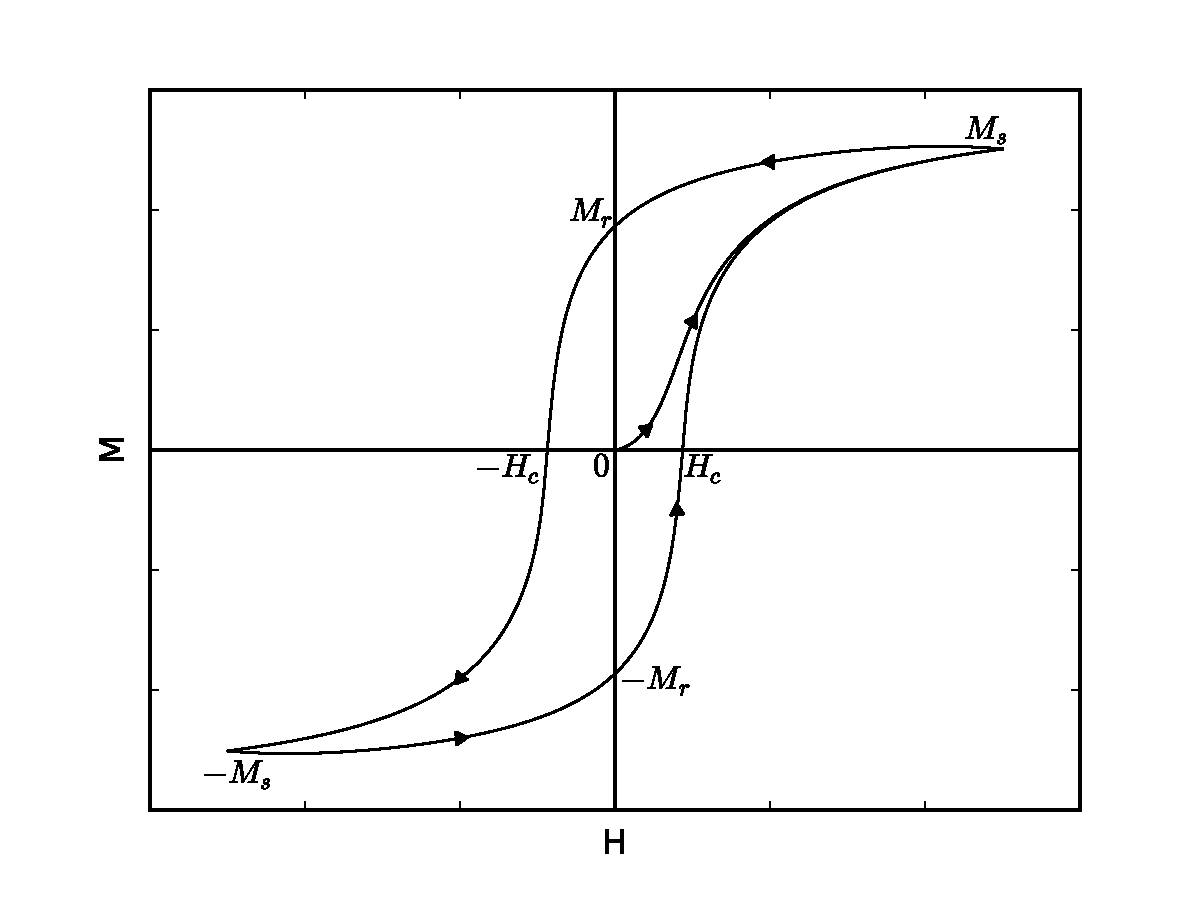
\includegraphics{figures/hysteresis_sample.pdf}}
\caption[Hysteresis loop of a ferromagnetic material]{Example of a hysteresis loop of a ferromagnetic material: $M_{r}$ is the remanent magnetization at H=0; ${H}_{c}$ is the coercivity, i.e. the reverse field that reduces $M$ to zero; $M_{s}$ is the saturation magnetization
\label{fig:hyst_loop}
}
\end{figure}

The upward curve starting at the origin is the inital magnetization curve which increases rapidly for increasing values of H until the saturation magnetization $M_{s}$ is reached. When H is now reduced, the magnetization decreases on a different curve. For a magnetic field intensity of zero the remanence magnetization $M_{r}$ is reached. In order to demagnetize the material a magnetic field, with a field intensity of $H_{c}$, also called the coercivity, must be applied in the opposite direction\cite{svoboda2004magnetic,sung2003physics,aharoni2000introduction}. \newline
Ferrimagnetic materials exhibit similar properties as ferromagentic materials as they both reach saturation and show much higher magnetization than either dia- or paramagnetic materials. As in ferromagnetic materials the magnetic moments are ordered regularly, but for ferrimagnetic materials in an antiparallel sense. However the opposing moments are unequal and a spontaneous magnetization still occurs. Ferrimagnetic behaviour is mainly shown by ferrites and mixed oxides of iron for example magnetite \cite{svoboda2004magnetic,michalowsky2006magnettechnik}.\newline
Ferro- and ferrimagnetic materials can also be divided by the value of their coercivity. Materials with a $H_{c}$ below 1\,kA/m are called magnetically soft, while materials with a larger value of $H_{c}$ are referred to as magnetically hard. Magnetically soft materials are easily magnetized and demagnetized, but exhibit only low remanent fields, in contrast magnetically hard materials will remain magnetized indefinitely unless they are demagnetized by an opposing magnetic field or heated above the Curie temperature \cite{meschede2015gerthsen}\cite{michalowsky2006magnettechnik}. 

\subsection{Influence of the particle shape and size}
\label{subsec:part_shape}
As already mentioned in Section\,\ref{subsec:Mag_mat}, the magnetic properties of ferromagnetic materials do not solely depend on the applied magnetic field, but also on the shape and size of the sample \cite{gomez2009influence}. The specific magnetic susceptibility $\chi$ is equivalent to $\kappa/\rho$, where $\kappa$ is the volume magnetic susceptibility and $\rho$ the material density. Therefore Equation\,\ref{eq:chi} can also be written as

\begin{equation}
\label{eq:kappa}
\centering
\boldsymbol{M} = \kappa\boldsymbol{H_{0}}
\end{equation}

where an external, homogeneous magnetic field with a magnetic field intensity of $H_{0}$ is applied. Here, $\kappa$ is not only dependent on the material, but also on the size and shape of the particle. The shape dependency can be explained by a demagnetizing field $H_{d}$ generated within the particle. The magnetic field $H_{i}$ inside the magnetized particle is not equal to the applied magnetic field $H_{0}$. The difference arises from the induction of a magnetic field $H_{d}$ inside of the finite ferromagnetic body of the particle opposing the external field. $H_{d}$ is proportional to $M$ as shown in Equation\,\ref{eq:demag_fac}. 

\begin{equation}
\label{eq:demag_fac}
\centering
\boldsymbol{H_{d}} = -N\boldsymbol{M}
\end{equation}

The dimensionless demagnetization factor $N$, with values in the range of 0 to 1, is dependent on the particle shape and the direction of magnetization. The inner magnetic field $H_{i}$ can therefore be calculated by Equation\,\ref{eq:int_field}. 

\begin{equation}
\label{eq:int_field}
\centering
\boldsymbol{H_{i}} = \boldsymbol{H_{0}} + \boldsymbol{H_{d}} = \boldsymbol{H_{0}} - N\boldsymbol{M}
\end{equation}

In case $N$ is known the magnetization of a material can be calculated solely from its material properties as shown in Equation\,\ref{eq:mag_demag_fac}. 

\begin{equation}
\label{eq:mag_demag_fac}
\centering
\boldsymbol{M} = \frac{\kappa{i}}{1+N\kappa_{i}}\boldsymbol{H_{0}}
\end{equation}

Where $\kappa$ from Equation\,\ref{eq:kappa} is substituted by the fraction $\kappa_{i}/(1+N\kappa_{i})$ with the intrinsic susceptibility $\kappa_{i}$, which is the true susceptibility after the removal of the effects of $H_{d}$ \cite{FranzrebHabil,svoboda2004magnetic}.\newline 
The magnetic properties of ferromagentic materials are not only influenced by the shape, but also by the size of the particles. When the particle size is sufficiently small, the particle will consist of only a single magnetic domain (for further explanations of magnetic domains see Section\,\ref{subsec:Mag_mat}). Single domain nanoparticles have been experimentally observed, for example by Majetich and Jin \cite{majetich1999magnetization}. The maximum diameter for spherical single domain particles is called the critical size. The critical size lies e.g. at approximately 0.05\,\textmu m for magnetite \cite{svoboda2004magnetic,butler1975theoretical}. Single domain particles are considered to be magnetized to saturation in one or the opposite direction, even if no external field is applied. Due to thermal motion the magnetization will fluctuate randomly between the two directions. This behaviour is called superparamagnetism.
Superparamagnetism is based on the same mechanism as paramagnetism, except that the magnetic moments are replaced by the moments of entire particles. Measurements of the magnetization of a larger number of superparamagnetic particles result in an observed net magnetization of zero, as the magnetization of each particle is oriented randomly. When an external field is applied, the moments of the particles will align and the net magnetization increases until saturation is reached. Once the field is removed, however, the particle moments will lose coherence and no net magnetization is retained. Consequently superparamagnetic particles show a coercivity and remanence of zero similar to paramagnetic materials combined with a high saturation magnetization comparable to ferromagnetic matter \cite{svoboda2004magnetic,FranzrebHabil}.      
    
\section{Fundamentals of magnetic separation}
\label{sec:Mag_sep}
Since the 19\textsuperscript{th} century magnetic separation processes have been used to concentrate and separate minerals. More recently, applications in waste water treatment, food industry and biotechnology have become available \cite{yavuz2009magnetic}. Magnetic separation technologies are used for the concentration of magnetic materials  as well as the removal of magnetizable particles from process fluids. For separation, the magnetic particles within a suspension are influenced by a non-homogeneous magnetic field, which leads to either retention or deflection of the particles. The external magnetic field can be generated by a permanent magnet or an electromagnet. In addition, the particles are influenced by other external forces e.g. gravitational, inertial, hydrodynamic and centrifugal forces (see Section\,\ref{subsec:bas_princ}). Furthermore electrostatic and electromagnetic interparticle forces affect the separation. Consequently, the magnetic force $F_{mag}$ must be greater than the sum of the competing forces $F_{comp}$ for successful separation of the particles from the surrounding fluid. For a selective separation of particles with different magnetic susceptibilities, the magnetic force acting on the more magnetic particles must be larger than the sum of $F_{comp}$ and for less magnetic particles smaller than the sum of $F_{comp}$. This condition is described in Equation\,\ref{eq:mag_sep_cond}, where $F_{mag}^{m}$ and $F_{mag}^{l}$ are the magnetic forces affecting the more and less strongly magnetic materials respectively and $F_{comp}$ summarizes the competing forces on the different particles \cite{svoboda2004magnetic,oberteuffer1974magnetic}.   

\begin{equation}
\label{eq:mag_sep_cond}
\centering
F_{mag}^{m}\geq\sum_{i}F_{comp}^{im} \quad \textrm{and} \quad F_{mag}^{l}\leq\sum_{i}F_{comp}^{il}
\end{equation}

In the following Section a more detailed explanation of the magnetic and the competing forces is given (see Section\,\ref{subsec:bas_princ}). In addition the basic concepts of \gls{hgms} and a simplified model approach are outlined in the Sections\,\ref{subsec:HGMS}, \ref{subsec:mag_field} and \ref{subsec:single_wire}.  

\subsection{Basic principles}
\label{subsec:bas_princ}
The concept of magnetic separation is based on the property of magnetic fields to exert a force on matter. The magnetic force $F_{m}$ on a particle is given by Equation \ref{eq:mag_force}

\begin{equation}
\label{eq:mag_force}
\centering
\boldsymbol{F}_{m} = \mu_{0}V_{p}\boldsymbol{M}_{p}\nabla\boldsymbol{H}
\end{equation}

where $V_{p}$ denotes the volume of the particle, $\boldsymbol{M}_{p}$ the particle magnetization and $\nabla\boldsymbol{H}$ the gradient of the applied magnetic field. For simplicity it is assumed that $F_{m}$ acts on the center of gravity of the particle. $\boldsymbol{M}_{p}$ can be calculated either by Equation\,\ref{eq:chi}, \ref{eq:kappa} or \ref{eq:mag_demag_fac}. As shown in Table\,\ref{table:mag_material}, the magnetic susceptibility for diamagnetic and paramagnetic materials is constant, while $\chi$ for ferromagnetic and ferrimagnetic substances is dependent on the magnetic field strength, the size and the shape of the particles (see Sections \ref{subsec:Mag_mat} and \ref{subsec:part_shape}). For spherical particles $F_{m}$ is also directly proportional to the cube of its radius $b$. \newline
As already mentioned above (see Section\,\ref{sec:Mag_sep}), the motion of the particles is also influenced by several different  forces. For ferromagnetic particles larger than approximately 1\,\textmu m the relevant competing forces are  the hydrodynamic drag force $F_{d}$, to a lesser degree in liquids the gravitational force $F_{g}$ and depending on the separator type the centrifugal force $F_{c}$.  


\begin{equation}
\label{eq:grav_force}
\centering
\boldsymbol{F}_{g} = (\rho_{p}-\rho_{f})V_{p}\boldsymbol{g}
\end{equation}

\begin{equation}
\label{eq:drag_force}
\centering
\boldsymbol{F}_{d} = 6\pi\eta b(\boldsymbol{v}_{f}-\boldsymbol{v}_{p})
\end{equation}

\begin{equation}
\label{eq:cent_force}
\centering
\boldsymbol{F}_{c} = (\boldsymbol{v}_{f}-\boldsymbol{v}_{p})\omega V_{p}\boldsymbol{r}
\end{equation}

$F_{g}$ for a spherical particle is given by Equation\,\ref{eq:grav_force}, where $g$ is the acceleration by gravity in m/s\textsuperscript{2} and $\rho_{p}$ and $\rho_{f}$ are the densities of the particle and the surrounding fluid in kg/m\textsuperscript{3}, respectively. The hydrodynamic drag force of a particle is determined by Stoke's law (see Equation\,\ref{eq:drag_force}), where $\eta$ denotes the dynamic viscosity of the fluid in Pa$\cdotp$s, $v_{f}$ the velocity of the fluid in m/s and $v_{p}$ the velocity of the particle in m/s. Stokes law is only valid for laminar flow around spherical objects with low Reynolds numbers and no interaction between the fluid and the particle. For our test cases low velocities and small particle sizes with no coupling between the particles were assumed and therefore Stokes law was applicable. $F_{c}$ is described by Equation\,\ref{eq:cent_force}, where $\omega$ is the angular velocity in rad/s and $r$ is the radial position of the particle. Equation\,\ref{eq:force_rad} shows the dependency of the different forces on the particle radius $b$ which could already be derived from Equation\,\ref{eq:grav_force} to \ref{eq:cent_force}. 

\begin{equation}
\label{eq:force_rad}
\centering
F_{g}\sim b^{3}, \quad F_{d}\sim b^{1} \quad \textrm{and} \quad F_{c}\sim b^{3}
\end{equation}

The equations show that $F_{g}$ and $F_{c}$ are directly proportional to the cube of the particle radius, consequently their contribution increases significantly with increasing particle size. $F_{d}$ however depends on the first power of the particle radius and will be relevant for smaller particles \cite{svoboda2004magnetic,oberteuffer1974magnetic}. For particles smaller than approximately 1\,\textmu m Brownian motion also needs to be considered. Brownian motion is the apparently random movement of particles in a fluid due to their collisions with other particles, atoms or molecules of the fluid \cite{brown1828xxvii}. The Langevin equation can be used for the description of Brownian motion (for more detailed information see \cite{Langevin,BrownianDynamics,BrownianModel}). It states that the minute fluctuations in the position of the particles are due to a random force. Einstein and Sutherland obtained a relation between the macroscopic diffusion constant $D$ and the atomic properties of matter \cite{einstein1906theorie,einstein1905molekularkinetischen,sutherland1905lxxv}. 

\begin{equation}
\label{eq:Stokes_Einstein}
\centering
D = \frac{k_{B}T}{6\pi\eta b}
\end{equation}

Equation\,\ref{eq:Stokes_Einstein}, called Stokes-Einstein equation, describes the diffusion of spherical particles through a fluid with low Reynolds numbers. $k_{B}$ is the Boltzmann constant with a value of 1.38064852$\cdotp$10\textsuperscript{-23}\,J/K, which can be calculated by the division of the universal gas constant $R$ by the Avogadro constant $N_{A}$, while $T$ is the temperature of the surrounding fluid. Particle diffusion can be pictured as a driving force which is based on the gradient in the particle concentration. 
A diffusion force $F_{B}$ acting on the particles can therefore be described by Equation\,\ref{eq:diff_force} as follows:

\begin{equation}
\label{eq:diff_force}
\centering
\boldsymbol{F}_{B} = -k_{B}T\frac{\nabla n}{n}
\end{equation}

where $n$ is the number density of particles within the fluid \cite{choomphon2017simulation,moeser2004high,fletcher1991fine}. \\ \newline
As the type of particles, defined by their shape, size and material, is usually given, the main influencing factors on $F_{m}$ for the magnetic separation are the magnetic field strength and its gradient. Consequently the combination of magnetic field strength and field gradient must be optimized for each application individually. The most common magnetic separators can be divided into three basic categories: open gradient magnetic separators, closed-gradient magnetic separators and matrix (polygradient) magnetic seperators \cite{svoboda2004magnetic}. \Gls{hgms}, which are used for the recovery of micron sized particles, belong to the class of matrix separators. In the following section the principles of \gls{hgms} will be further explained.  


\subsection{High gradient magnetic separation}
\label{subsec:HGMS}
In conventional magnetic separators only ferromagnetic materials with a particle size larger than approximately 50\,\textmu m can be separated. \Gls{hgms}, based on the Frantz Ferrofilter, enables the magnetic separation of smaller and only weakly magnetic particles \cite{frantz1937patent,ge2017magnetic}. This is achieved through the combination of strong magnetic fields and high magnetic field gradients. Ferromagnetic bodies, called the matrix, are placed in the external magnetic field. The applied magnetic field induces magnetic moments in the ferromagnetic matrix which leads to high magnetic field gradients in the proximity of the matrix elements \cite{shukla2006process}. Magnetically susceptible particles move along the gradient towards the magnetized matrix elements and are captured on the surface \cite{hoffmann2002novel}. As the magnitude of the magnetic field gradient as well as the collection surface are dependant on the shape, size, arrangement and placement of the used bodies, the matrix material e.g. balls, grooved plates, steel wool or rods has to be chosen carefully (more information on different matrix materials can be found in \cite{iacob2002high,kim2013effects,takayasu1981matrices}). The matrix has to be fine enough to generate a strong enough magnetic field gradient for selective separation, but also not so strong as to cause matrix blockage and retention of non-magnetic materials. As the filling factor of the used matrix material is often low, e.g. 0.04 and 0.20 for steel wool and expanded metal respectively and as the matrix does not conduct magnetic flux very well, strong external fields are required. An exception are matrices consisting of balls with a filling factor of up to 0.50 and grooved plates with a filling factor of 0.80. 
%In general, the separation efficiency of ball matrices is smaller than the in filament units, as a closed packed array of spheres does not leave much space for the collection of particles.  


%%%%%%%%%%%%Include Figure of HGMS%%%%%%%%%%%%%%%%%%%%%%%%%%%%%%%%%%%%%%%%%%%%%%%%%%%%%%change figure !!!!!!!!!!!!!!!!!

\begin{figure}[H]
\centering

\scalebox{0.35}{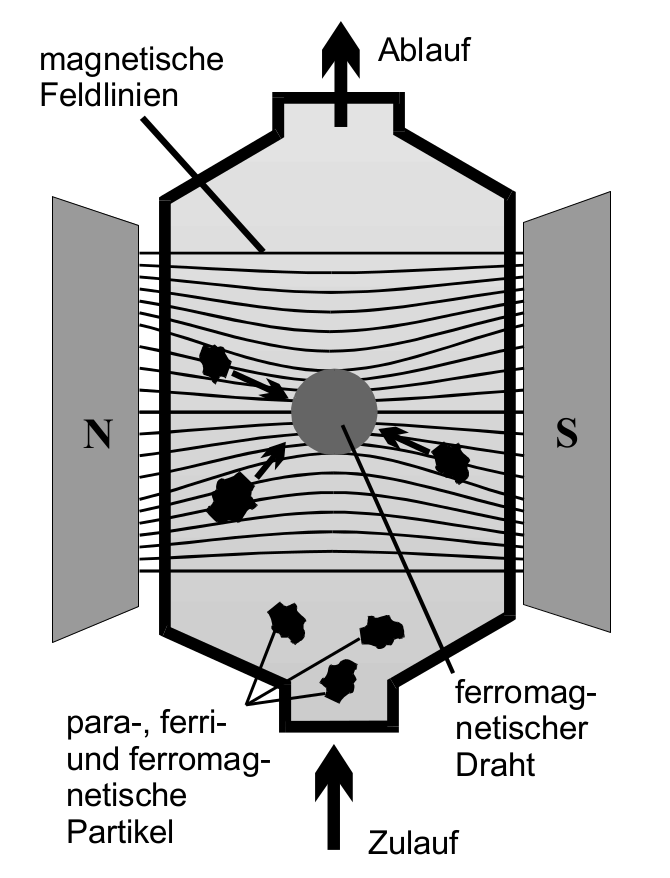
\includegraphics{figures/hgms_franzreb.png}}
\caption[Schematic HGMS process]{Schematic HGMS process: The ferromagnetic wire is placed in the external field generated by permanent magnets. It generates high magnetic field gradients. The magnetic particles in the suspension move along the gradient towards the wire and are captured on the wire's surface (modified from \cite{FranzrebHabil}).  
\label{fig:hgms}
}
\end{figure}

A schematic drawing of a \gls{hgms} is shown in Figure\,\ref{fig:hgms}. The particle suspension flows through the matrix. Particles with high magnetic susceptibilities accumulate on the matrix surface while the rest of the suspension leaves the system. Once the matrix is saturated with particles, the external magnetic field is turned off and the collected particles are recovered \cite{svoboda2004magnetic,gerber1983high,ditsch2005high}. \gls{hgms} can be modeled by a simplified setup of a single magnetized, ferromagnetic wire which is surrounded by the flowing particle suspension. %welches von der Partikelsuspension umströmt wird  

\subsection{Magnetic field in the vicinity of a magnetized wire}
\label{subsec:mag_field}
The magnetic field $H(r,\varphi)$ in the vicinity of a infinitely long cylinder, which is magnetized by a homogeneous magnetic field $H_{0}$ (configuration shown in Figure\,\ref{fig:wire}), is described by the following equation\,\ref{eq:mag_field_strat}:

\begin{equation}
\label{eq:mag_field_strat}
\centering
H = H_{0}(e_{r}cos\varphi-e_{\varphi}sin\varphi)+H_{0}\frac{a^{2}}{r^{2}}\left(\frac{\mu_{w}-\mu_{f}}{\mu_{w}+\mu_{f}}\right)(e_{r}cos\varphi+e_{\varphi}sin\varphi)
\end{equation}

where $e_{r}$ and $e_{\varphi}$ are the unit vectors in the polar coordinate system and $\mu_{w}$ and $\mu_{f}$ depict the magnetic permeability of the wire and the fluid, respectively \cite{stratton2007electromagnetic}. For an external field $H_{0}$, that is strong enough to magnetize the wire to saturation, and a surrounding medium with a permeability close to one, e.g. water or air, Equation\,\ref{eq:mag_field_strat} can be written as follows in Equation\,\ref{eq:Hr_field} and \ref{eq:Hphi_field}:

\begin{equation}
\label{eq:Hr_field}
\centering
H_{r} = \left(\frac{M_{s,w}a^{2}}{2r^{2}}+H_{0}\right)cos\varphi
\end{equation}
%%%%%%%%%%%%%%%%sin\theta ???cos\theta????????%%%%%%%%%%%%%%%%%%%%%%%%%%%%%%%%%%%%
\begin{equation}
\label{eq:Hphi_field}
\centering
H_{\varphi} = \left(\frac{M_{s,w}a^{2}}{2r^{2}}-H_{0}\right)sin\varphi
\end{equation}

where $a$ is the radius of the wire and $r$ is the distance between the wire and the magnetic nanoparticle \cite{FranzrebHabil}. The magnetic field of a magnetized ferromagnetic wire is shown in Figure\,\ref{fig:mag_field_wire}. The magnetic force $F_{m}$ affecting the particles can then be calculated from the magnetic field with Equation\,\ref{eq:mag_force} \cite{moeser2004high}. 

\begin{figure}[H]
\centering
\scalebox{0.4}{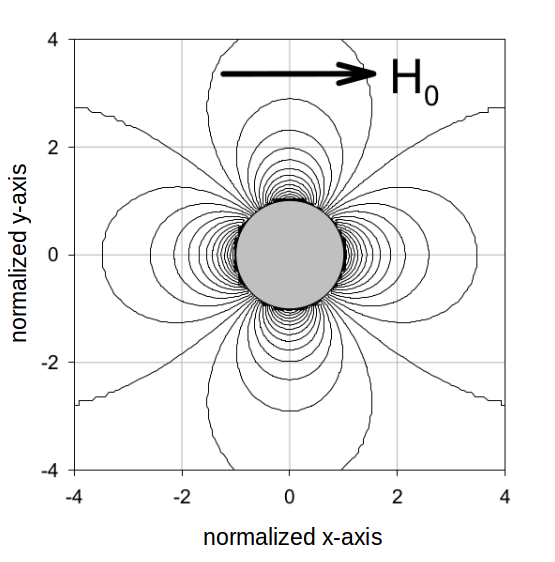
\includegraphics{figures/mag_field_wire_franz_modified.png}}
\caption[Magnetic field in the vicinity of a wire]{Field lines of a magnetic field in the vicinity of a magnetized ferromagnetic wire (modified from\cite{FranzrebHabil})
\label{fig:mag_field_wire}
}
\end{figure}


\subsection{Magnetic particle accumulation on single wires}
\label{subsec:single_wire}
For micron-size particles or larger, the capture process in \gls{hgms} can be simplified by the analysis of a single magnetized collector and the particle trajectories in its vicinity. Figure\,\ref{fig:wire} depicts the configuration of particle capture in a single wire model.

\begin{figure}[h]
\centering
\scalebox{0.3}{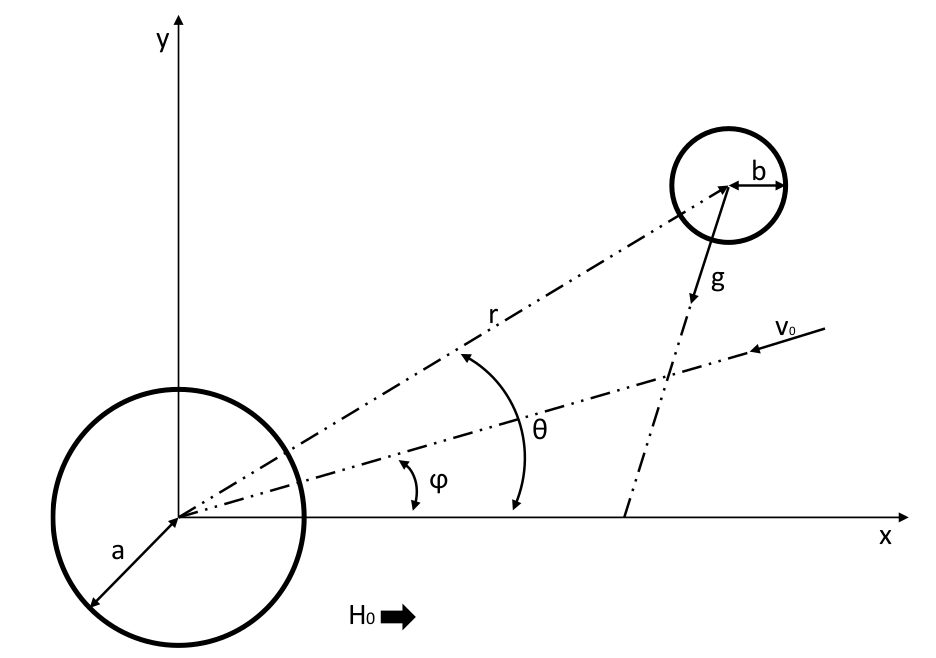
\includegraphics{figures/Single_wire.png}}
\caption[Configuration of particle capture in a single wire model]{Configuration of particle capture in a single wire model: A cylindrical ferromagnetic wire with the radius $a$, which is magnetized to saturation by an external magnetic field $H_{0}$, a paramagnetic particle with the radius $b$ at a distance $r$ from the wire and a polar angle of $\theta$ from the wire center and the fluid flow velocity $v_{0}$ \cite{svoboda2004magnetic}
\label{fig:wire}
}
\end{figure}

For a single wire model three different orientations of the wire relative to the flow and applied field are considered. It is assumed that the magnetic field is always orthogonal to the ferromagnetic wire. The direction of the fluid flow can then be either parallel (longitudinal) or perpendicular (transversal) to the direction of the magnetic field. In addition, the fluid flow can be oriented parallel to the wire, which is referred to as axial configuration \cite{friedlaender1978particle}. The particle build-up profiles for the three different orientations are shown in Figure\,\ref{fig:hgms_config}.   

\begin{figure}[h]
\centering

\scalebox{0.40}{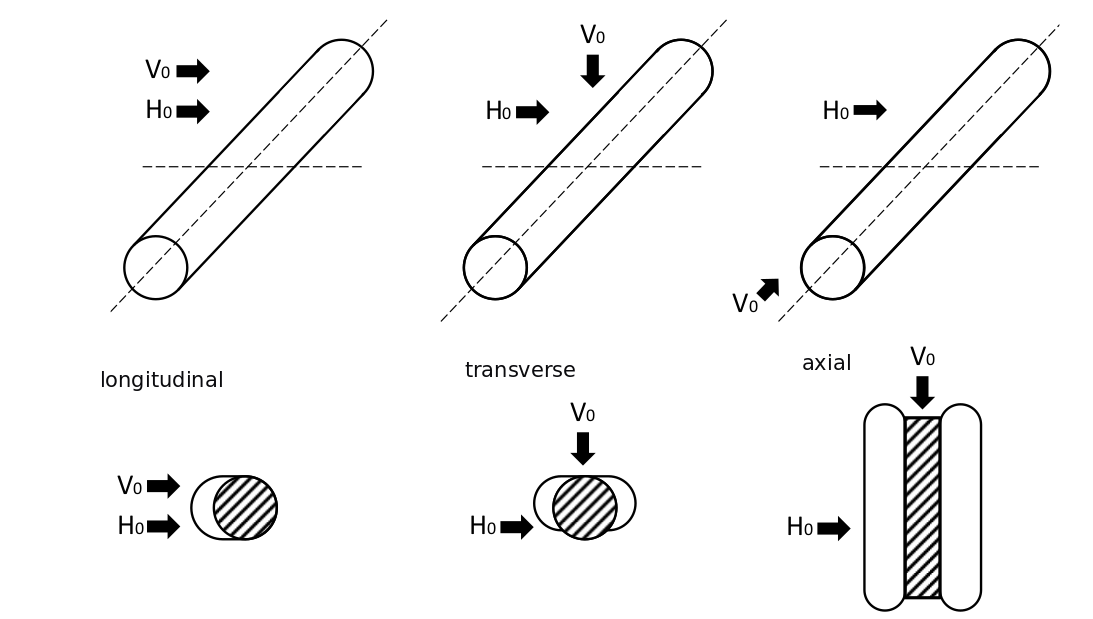
\includegraphics{figures/hgms_orientation.png}}
\caption[Geometric configurations in HGMS and particle build-up]{Schematic drawing of the three main geometric configurations in HGMS and the corresponding profiles of the particle build-up in a ferromagnetic wire; arrangements between the directions of the magnetic field $H_{0}$ and the particle flow velocity $v_{0}$ with respect to the wire (top) and the cross section of the wire (hatched area) with the particle build-up profile corresponding to the respective configuration \cite{svoboda2004magnetic}
\label{fig:hgms_config}
}
\end{figure}

The particle trajectories in the vicinity of the wire are calculated by Newton's second law, which states that the sum of all forces affecting the particle is equal to the product of the particle mass $m$ and its acceleration $a_{p}$. 

\begin{equation}
\label{eq:mag_force_sum}
\centering
\sum_{i}\boldsymbol{F}_{i} = m\boldsymbol{a}_{p}
\end{equation}
 
The forces acting on the particles e.g. the magnetic, gravitational and hydrodynamic force are described in Section\,\ref{subsec:bas_princ}. Whether a particle is collected by the wire or not can be determined by following the particle trajectory. If the particle trajectory ends on the wire's surface, the particle is separated, if, however, the particle trajectory passes the wire the particle remains in suspension \cite{FranzrebHabil}. A model for particle trajectories with a sphere instead of a wire can be found in \cite{friedlaender1981particle,moyer1986filtration}. \newline 
In the case of ultra-fine magnetic particles, where the diffusion outweighs the other forces, the trajectory analysis is not suitable. In this case, the continuity equation representing the conservation of mass with the influence of external forces on individual magnetic particles expressed through the flux term is solved \cite{choomphon2017simulation}. In a two-dimensional model spherical and cylindrical collectors are show the same results. The solution of the continuity equation, describing the time-dependent distribution of the magentic particles around the collector, can be written as follows in Equation \ref{eq:diff_eq}:     

\begin{equation}
\label{eq:diff_eq}
\centering
\frac{\partial n}{\partial t} = \nabla\cdotp(D\nabla n)-\nabla\cdotp(n v_{p})
\end{equation}

where $n$ is the particle number density, $D$ the diffusion coefficient and $v_{p}$ the particle drift velocity caused by the magnetic force $F_{m}$ for spherical particles at low Reynolds numbers \cite{fletcher1991fine,FranzrebHabil}. $D$ is determined by the Stokes-Einstein relation (see Section\,\ref{subsec:bas_princ}). For a steady-state, i.e. ${\partial n}/{\partial t}$=0, Equation\,\ref{eq:diff_eq} reduces to:

\begin{equation}
\label{eq:diff_eq_2}
\centering
 D\nabla n = n v_{p}
\end{equation}

which describes the dynamic balance between an inward flux of the particles towards the wire and an outward flux due to Brownian motion \cite{fletcher1991fine}. 



% Diffusion with force balance: \cite{gerber1983generalization}\cite{takayasu1983magnetic}\cite{davies19902}\cite{fletcher1991fine}
% Diffusion with energy model \cite{glew1984influence}
% 
%  \cite{choomphon2017simulation}
% \cite{moyer1986filtration} for spheres as matrix


% \section{Dimensioning of a Helmholtz coil}
% \label{sec:Dim_helm_coil}
% A Helmholtz coil produces an approximately uniform magnetic field along the x-axis between the coils. The dimensioning of the coil is based on the Biot-Savart law, which describes the magentic field generated by a stationary electric current. The magnetic flux density in a cylindrical coil with only one winding can be calculated with Equation \ref{eq:one_winding}. 
% 
% \begin{equation}
% \label{eq:one_winding}
% \centering
%  B(r) = \frac{\mu_{0}}{4\pi}\int d^{3}r^{'}j(r^{'}\times \frac{r-r^{'}}{\vert r-r^{'} \vert^{3}}
% \end{equation}
% 
% Where $d^{3}r^{'}$ denotes a volume integral, $j(r^{'}$ the current density and $r-r^{'}$ a direction vector. In addition the vectors $r$ and $r^{'}$ are defined as the following: $r = (0,0,z)$ and $r^{'} = (R cos(\phi),R sin(\phi), z^{'})$. 
% 
% \cite{wotruba1968verbesserung}\cite{wotruba1969massive}\cite{heller1955erzeugung}
%%%%%%%%%%%%%%%%%really necessary??%%%%%%%%%%%%%%%%%%%%%%%%%%%%%%%%%%%%%%%%

\section{Computational fluid dynamics}
\label{sec:CFD}
\Gls{cfd} is a well established method in fluid mechanics. It enables a quick and efficient analysis of fluid flows. Formerly mainly used for numerical weather prediction or calculations concerning the aerodynamics of airplanes, it has now become a vital component in process and
product development in many different aspects of engineering. Applications vary from chemical process and civil engineering to biomedical and pharmaceutical
process and product design. CFD offers an inexpensive alternative or addition to experimental approaches as well as the possibility to study systems in which experiments would be unfeasible. Other main advantages include the reduced time, parallel processing and the almost unlimited level of detail of the results. The progress in both hardware and numerical algorithms in the past decades has led to the development of numerous commercial and open-source CFD programs \cite{ghia1982high}. In this work a numerical model using the COMSOL Multiphysics  software (COMSOL Inc., Stockholm, Sweden), which is a predominantly finite element analysis, solver and simulation package specialized for coupled phenomena and multiphysics, was developed.

\subsection{Navier-Stokes equations}
\label{subsec:Navier_Stokes}
The Navier-Stokes equations are a macroscopic model of the motion of viscous fluids and the basis of the fluid-dynamic calculations of COMSOL. Analytical solutions only exist for simplified versions of the Navier-Stokes equations e.g. Couette flow and Hagen-Poiseuille flow. For more complex, nonlinear problems like the setup in this thesis the equations need to be solved numerically. The Navier-Stokes equations in their most general form for a compressible fluid can be written as follows in Equations \ref{eq:Conservation of momentum 1}, \ref{eq:Conservation of mass 1} and \ref{eq:Conservation of energy 1}:

% \begin{equation}
% \rho\frac{\partial \boldsymbol u}{\partial t} + \rho\boldsymbol u\cdotp\nabla\boldsymbol u - \left(\mu(\nabla\boldsymbol u+(\nabla\boldsymbol u)^{T})-\frac{2}{3}\mu(\nabla\cdotp\boldsymbol u)\boldsymbol I\right) + \nabla p = \boldsymbol F
% \label{eq:Conservation of momentum 1}
% \end{equation}

\begin{equation}
\rho\frac{\partial \boldsymbol u}{\partial t} + \rho\boldsymbol u\cdotp\nabla\boldsymbol u - \nabla\cdotp[-p\boldsymbol I + \boldsymbol \tau] = \boldsymbol F
\label{eq:Conservation of momentum 1}
\end{equation}


\begin{equation}
\frac{\partial\rho}{\partial t}+\nabla(\rho\boldsymbol u) = 0
\label{eq:Conservation of mass 1}
\end{equation}

\begin{equation}
\rho C_{p}\left(\frac{\partial T}{\partial t}+(\boldsymbol u \cdotp\nabla)T\right) = -(\nabla\cdotp\boldsymbol q)+\tau:\boldsymbol S -\frac{T}{\rho}\left.\frac{\partial p}{\partial t}\right\vert_{p}\left(\frac{\partial p}{\partial t}+(\boldsymbol u\cdotp\nabla)p\right)+Q 
\label{eq:Conservation of energy 1}
\end{equation}

where $\rho$ is the density in kg/m\textsuperscript{3}, $\boldsymbol u$ is the velocity in m/s, $p$ is the pressure in Pa, $\tau$ is the viscous stress tensor in Pa, $\boldsymbol I$ is the unit vector, $\boldsymbol F$ is the volume force vector in N/m\textsuperscript{3}. $C_{p}$ is the specific heat capacity in at constant pressure in J/(kg$\cdotp$K), $T$ is the absolute Temperature in K, $\boldsymbol q$ is the heat flux vector in W/m\textsuperscript{2}, $Q$ describes the heat sources in W/m\textsuperscript{3} and $\boldsymbol S$ is the strain-rate tensor. The Navier-Stokes Equations (see Equation\,\ref{eq:Conservation of momentum 1}) satisfy the conservation of momentum, while the continuity equation (see Equation\,\ref{eq:Conservation of mass 1} represents the conservation of mass. Equation\,\ref{eq:Conservation of energy 1} describes the conservation of energy formulated in terms of temperature. The double dot product describes the contraction between two tensors. The strain-rate tensor can be calculated by the expression in Equation\,\ref{eq:strain_tensor}.

\begin{equation}
\boldsymbol S = \frac{1}{2}(\nabla\boldsymbol u+(\nabla\boldsymbol u)^{T})
\label{eq:strain_tensor}
\end{equation}

Newtonian fluids exhibit a linear correlation between the viscous stress, arising from its flow, and the local strain-rate, which is described by Equation\,\ref{eq:stress_tensor}, where $\mu$ is the dynamic viscosity in Pa$\cdotp$s.

\begin{equation}
\boldsymbol\tau = 2\mu\boldsymbol S - \frac{2}{3}\mu(\nabla\cdotp\boldsymbol u)\boldsymbol I
\label{eq:stress_tensor}
\end{equation}

For incompressible Newtonian fluids, like water or alcohol, the Equations\,\ref{eq:Conservation of momentum 1} and \ref{eq:Conservation of mass 1} are reduced to Equations\,\ref{eq:Conservation of momentum } and \ref{eq:Conservation of mass }\cite{versteeg2007introduction}. 

\begin{equation}
{\partial{\boldsymbol u}\over{\partial t}} + ({\boldsymbol u} \cdot \nabla) {\boldsymbol u} - \nu\Delta{\boldsymbol u}+ \frac{1}{\rho}\nabla p = {\boldsymbol F}
\label{eq:Conservation of momentum }
\end{equation}

\begin{equation}
\nabla{\boldsymbol u} = 0
\label{eq:Conservation of mass }
\end{equation}
 
The first term describes the local acceleration of the fluid, $({\boldsymbol u} \cdot \nabla) {\boldsymbol u}$ the non-linear convective term, representing the inertial forces, $\nabla p$ the pressure gradient and $\nu\Delta{\boldsymbol u}$ the dissipative viscous term. The Navier-Stokes equations are always solved together with the continuity equation (see Equation\,\ref{eq:Conservation of mass }). 
%The Navier-Stokes equations satisfy the conservation of momentum, while mass conservation is included through the continuity equation \cite{alkahtani2013numerical}.
The Reynolds number is a dimensionless quantity in fluid dynamics, which is used to characterize a fluid flow. The Reynolds number is defined as the ratio of the inertial forces to the viscous forces and can be written as follows (Equation\,\ref{eq:Reynolds}):  

\begin{equation}
Re=\frac{\rho u L}{\mu}=\frac{uL}{\nu}
\label{eq:Reynolds}
\end{equation}

where $\rho$ is the fluid density in kg/m\textsuperscript{3} and $L$ is a characteristic linear dimension in m, e.g. the hydraulic diameter of a pipe. For a low Reynolds number the flow condition will be laminar, while for higher Reynolds numbers, above approximately 2300 for a flow in a circular pipe, turbulent flow occurs \cite{schwarze2012cfd}. Flows where Re is much smaller than one are referred to as Stokes flow or creeping flow. Here the viscous forces are much larger than the inertial forces which is usually caused by either very low velocities or small characteristic lengths, f.e. in microfluidics. Stokes flow also occurs in highly viscous fluids such as heavy oils and honey \cite{lautrup2004physics}. Figure\,\ref{fig:creep_tot} shows creeping flow around a cylinder, with its characteristic streamlines, that are parallel to the surface of the cylinder as a schematic drawing and in reality. A turbulent flow around the same cylinder, which would occur e.g. for large u, would appear less ordered and contain eddies or swirls.

\begin{figure}[h]
		%\centering
          \begin{subfigure}{0.49\textwidth}
                  \flushleft
                  \scalebox{0.13}{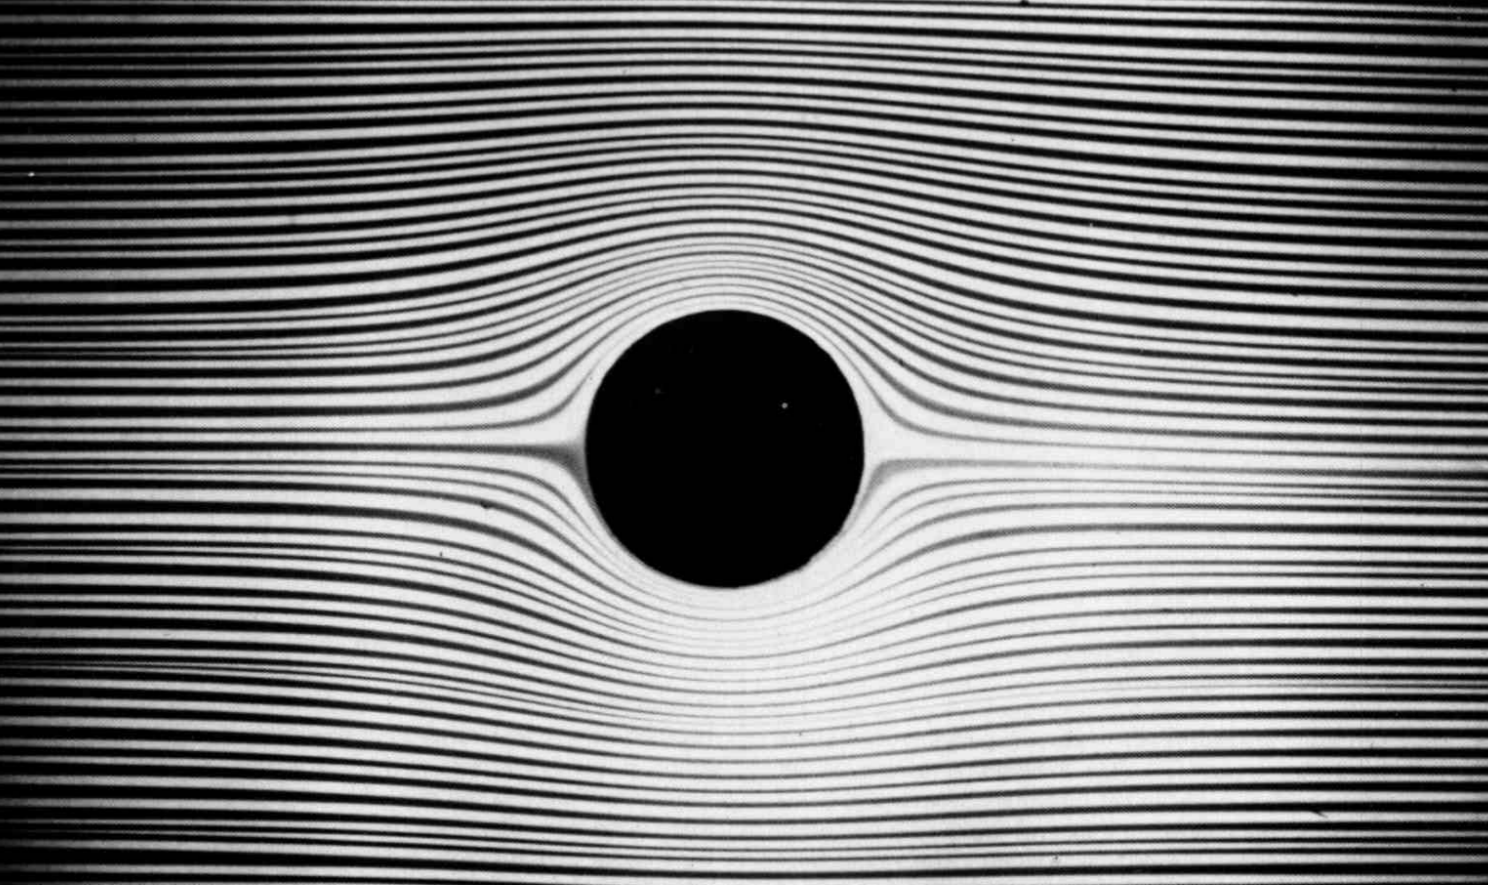
\includegraphics{figures/Creeping_flow_around_Cylinder.png}}
                  \caption{Streamlines in water flowing past a cylinder with a velocity of 1\,mm/s between glass plates placed 1\,mm apart visualized with dye \cite{van1982album}\label{fig:creep_1}}
          \end{subfigure}\hfill
        \begin{subfigure}{0.49\textwidth}
                \flushright
                \scalebox{0.358}{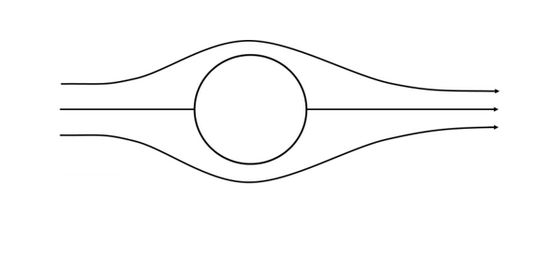
\includegraphics{figures/Creeping_flow_around_cylinder_schematic_4.png}}
                \caption{Schematic drawing of the streamlines around a cylinder for creeping flow}\label{fig:creep_2}
        \end{subfigure}
        \\
        
        \caption[Creeping flow around a cylinder]{Streamlines of the flow field for a creeping flow around a cylinder with Re\,$\ll$\,1 }
        \label{fig:creep_tot}
  \end{figure}

\subsection{Space and time discretization methods}
\label{subsec:FEM}
Space and time dependent physical problems are usually described with the help of \glspl{pde} in a domain $\Omega$. Most of these \glspl{pde} cannot be solved with analytical methods, but an approximation of the equations based on different types of discretizations can be obtained. \Gls{fem} is a numerical technique for constructing such approximate solutions for \glspl{pde}. The principle of the method is to replace an entire continuous domain by a number of finite-sized subdomains, called elements, of geometrically simple shapes like tetrahedrons or triangular prisms. Together the elements constitute a finite-element mesh. The \glspl{pde} for each element are approximated by an interpolation function, such as a linear, quadratic or higher order polynomial, also referred to as basis function, with a finite number of degrees of freedom. In combination with the boundary conditions a  system of algebraic equations is obtained, which can be solved by a sparse matrix solver \cite{john2016finite}. The solution of the matrix results in an approximate solution of the \glspl{pde}. The accuracy of the solution can be increased by a refinement of the finite-element mesh or an increased order of the basis function. An example of the approximation of a function $u$ by the function $u_{h}$ consisting of linear combinations of basis functions $\psi_{i}$ with the coefficients $u_{i}$ (see Equation\,\ref{eq:FEM}) is depicted in Figure\,\ref{fig:FEM}. 

\begin{equation}
u\approx u_{h} \quad \textrm{with} \quad u_{h}=\sum_{i}u_{i}\psi_{i}
\label{eq:FEM}
\end{equation}

\begin{figure}[H]
\centering
\scalebox{0.3}{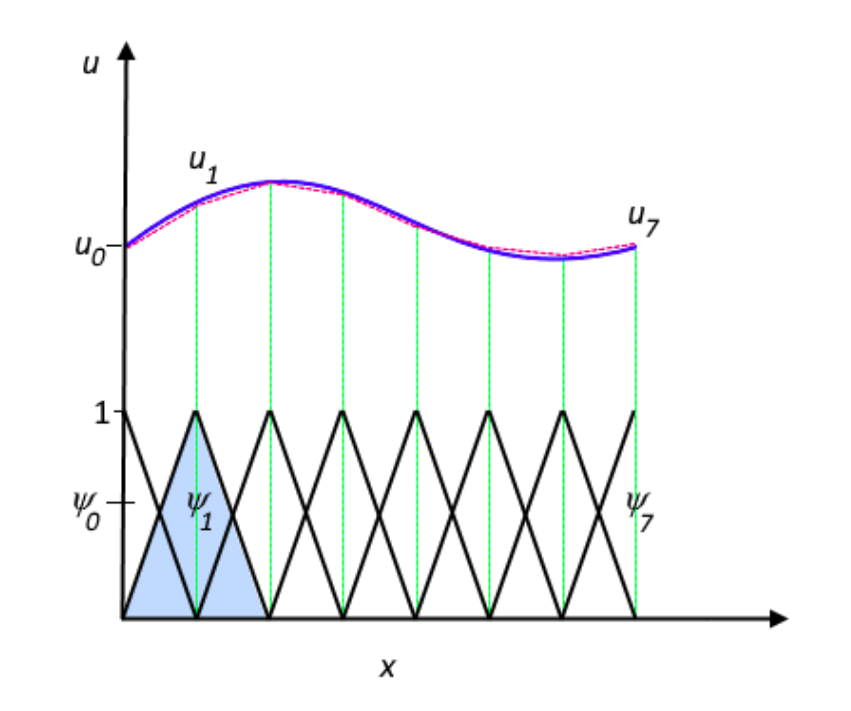
\includegraphics{figures/FEM.png}}
\caption[Approximation of a function with FEM]{Approximation of the function $u$ (solid blue line) by the function $u_{h}$ (dashed red line), where $u_{h}$ is a combination of linear interpolation functions $\psi_{i}$ (solid black lines) and the coefficients $u_{0}$ to $u_{7}$ \cite{ComsolFEM}
\label{fig:FEM}
}
\end{figure}

Overall \gls{fem} for the approximation of \glspl{pde} can be divided into four steps: discretization of the domain, selection of the interpolation functions, formulation of the system equations and solution of the system equations. \newline 
\Gls{fem} can also be applied for a time domain, this can, however, come at the cost of a high computational effort. Therefore simple time-stepping methods based on finite differences are frequently used for time discretization. The implicit time-stepping algorithm used in this work is the \gls{bdf} solver, which uses backward differentiation formulas with the order of accuracy varying from one, known as the backward Euler method, to five. \gls{bdf} solvers exhibit a high stability, but also include more damping effects than comparable solvers based on e.g. generalized alpha or Runge-Kutta methods \cite{ComsolRefManual}.

\section{Analysis of peak asymmetry}
\label{sec:peak_as}
In chromatography, the peak shape is extremely important, as it can be used to extract basic performance parameters such as the peak height, area, resolution and asymmetry. For the experimental setup in this thesis mainly the retention time, peak area and asymmetry were evaluated (for more information on the setup and evaluation methods see Section\,\ref{sec:Exp_setup}). In the following, the asymmetry of chromatographic peaks is further discussed. \newline 
An idealized chromatographic peak with a Gaussian profile is depicted in Figure\,\ref{fig:peak_param}. As most real chromatographic peaks are not symmetrical, an asymmetry factor $A_{s}$ is introduced to characterize the peak shape and to evaluate the quality of the packed bed. The asymmetry can be empirically determined by $A_{s}=b/a$, where $a$ is the partial peak width of the first part, measured at a certain percentage of the peak height and $b$ is the partial peak width for the secodn part of the peak, also measured at the same percentage of height. $A_{s}$ is usually measured at 10\,\% of the peak height as for Gaussian and near Gaussian peaks it results in much more accurate values with lower standard deviations as compared to measurements at 5, 30 or 50\,\% \cite{foley1983equations}. The Gaussian standard deviation of the asymmterical peak can be estimated with Equation \ref{eq:Gaus_dev}, where $w_{10}=a+b$ is the peak width at $h_{10}$ \cite{papai2002analysis}.  

\begin{equation}
\sigma=\frac{w_{10}}{3.27 b/a + 1.2}
\label{eq:Gaus_dev}
\end{equation}

\begin{figure}[h]
\centering
\scalebox{0.6}{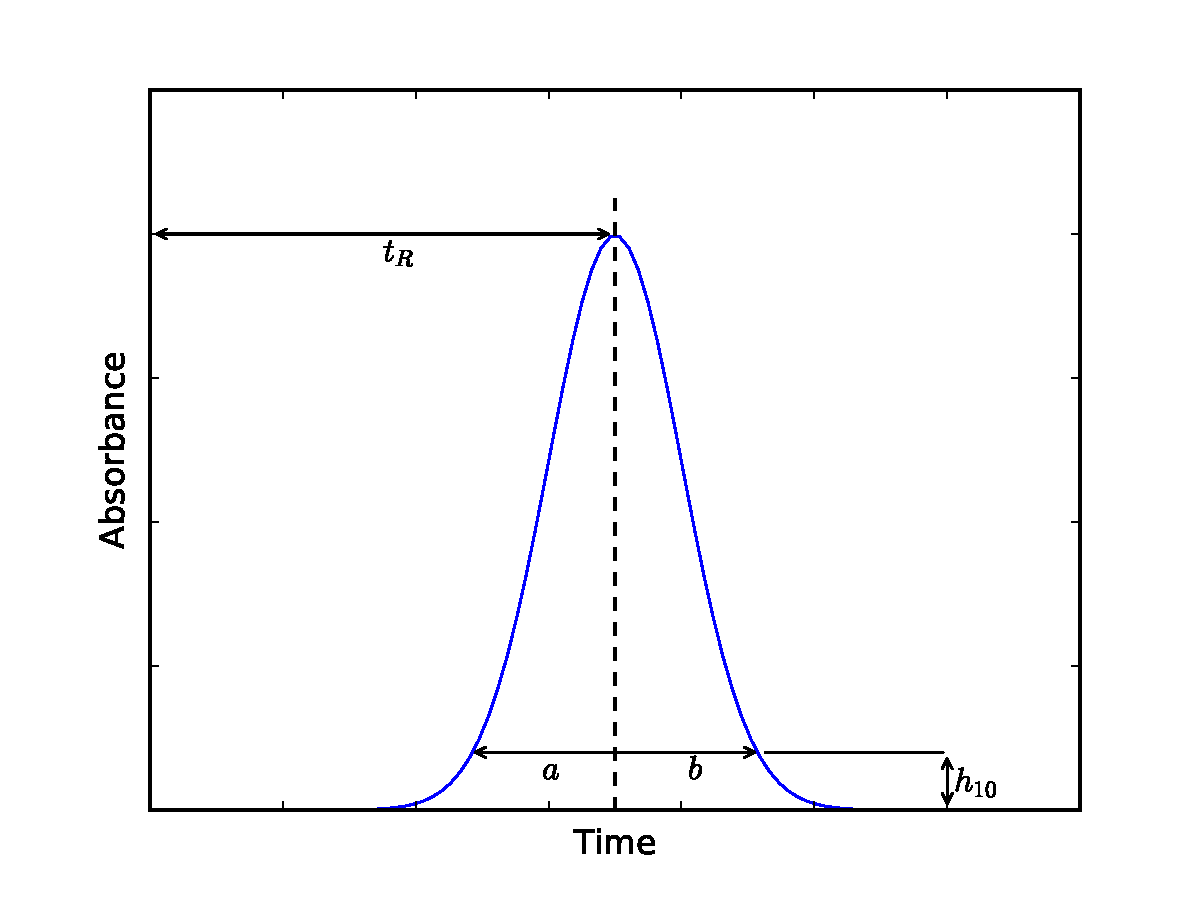
\includegraphics{figures/Peak_param.pdf}}
\caption[Idealized chromatographic peak]{Idealized chromatographic peak: Measurement of the retention time $t_{R}$ and the asymmetry factor $A_{s}=b/a$ at 10\,\% peak height $h_{10}$.  
\label{fig:peak_param}
}
\end{figure}

The peak shape for values of $A_{s} < 1$ is called fronting and for values of $A_{s} > 1$ tailing. Tailing is e.g. caused by dead volume in the flow path or the column packing, while fronting can arise from channeling in poorly packed columns. Therefore $A_{s}$ is a good indicator of the quality of the packed bed and should be checked regularly before each experimental cycle. As almost all chromatographic peaks tail to some extent, an acceptable range for $A_{s}$ has to be defined for each column and application individually.  

% \section{Simulated moving bed chromatography}
% \label{sec:smb}
% The overall goal of the research project this thesis is embedded in is to develop a continuous size fractionation process for magnetic nanoparticles at industrial scale. \Gls{smb} is a continuous countercurrent chromatography method, which was developed in the late 1950s by engineers from Universal Oil Products to separate p-xylene from its isomers \cite{broughton1961continuous,carson1962rotary}. The invention of the continuous process was mainly motivated by the need to produce large quantities of chemicals at high purity in a comparatively short time. Since the 1990s \gls{smb} is increasingly used in other industries than petrochemistry, e.g. cane and beet molasse separation in the sugar industry or the production of enantiomerically pure drugs in the pharmaceutical industry. The principle of countercurrent chromatography is depicted in Figure\,\ref{fig:SMBTurtle}. The process of separation of two components can be illustrated by picturing a fast cat and a slow turtle running on a conveyor belt that is moving in the opposite direction. The velocity of the cat is larger than and the velocity of the turtle is smaller than the velocity of the conveyor. Therefore the cat will move to the right side, while the turtle is dragged to the left side of the band and thus they are separated \cite{rajendran2009simulated}.  
% 
% \begin{figure}[H]
% \centering
% \scalebox{0.67}{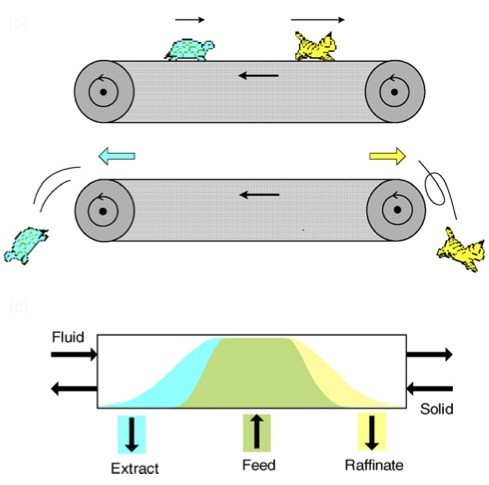
\includegraphics{figures/SMBTurtle.jpg}
% \caption[Principle of counter current chromatography]{Principle of counter current chromatography: the cat-turtle separator (top and middle) and a schematic for countercurrent chromatography (bottom) \cite{rajendran2009simulated}}
% \label{fig:SMBTurtle}
% }
% \end{figure}
% 
% 
% The same separation of components is achieved in a continouse countercurrent chromatography column, where both the fluid and the solid are pumped into opposite directions. The component mixture is fed continuously to the middle of the column and the two seperated components are collected on either side of the column \cite{deckert1994simulierte}. As pumping of the solid phase is neither easy to achieve nor practicable the column is substituted by several seperate columns and the movement of the bed is simulated by either moving the columns on a caroussle like structure or switching of the inlet and outlet flows with rotray valves \cite{SWB-414874366}. A schematic four column setup for a \gls{smb} process is shown in Figure\,\ref{fig:SMB}.
% 
% \begin{figure}[H]
% \centering
% \scalebox{0.67}{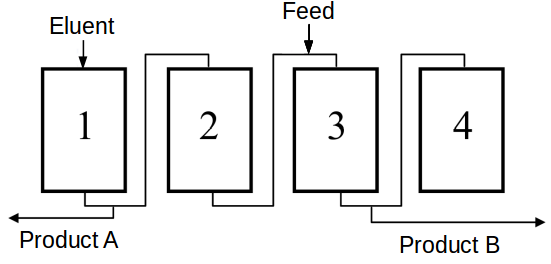
\includegraphics{figures/smb_schema.png}
% \caption[Schematic drawing of a SMB process]{Schematic drawing of a SMB process, where a feed consisting of the more retained product A and the less retained product B is split into two pure fractions of the products}
% \label{fig:SMB}
% }
% \end{figure}
% 
% With this setup a continuous binary separation of a mixture can be achieved with high purity and yield. The projects objective is to apply the \gls{smb} method on columns with a magnetizable packed bed matrix in order to achieve a continuous size fractionation of magnetic particles in the nanoparticle range.   


\chapter{Materials and Methodology}
\label{chap:chap_mat}
\newacronym{pva}{PVA}{polyvinyl alcohol}
\newacronym{pmma}{PMMA}{polymethyl methacrylate}
\newacronym{ptfe}{PTFE}{polytetrafluorethylen}
\newacronym{fplc}{FPLC}{fast protein liquide chromatography}
\newacronym{esem}{ESEM}{environmental scanning electron microscope}
\newacronym{agm}{AGM}{alternating gradient magnetometer}
\newacronym{mumps}{MUMPS}{multifrontal massively parallel sparse direct solver}
\newacronym{pardiso}{PARDISO}{parallel direct sparse solver}

In the first part of this chapter the model setup and implementation using the simulation software COMSOL Multiphysics\textsuperscript{\textregistered}, thereafter referred to as COMSOL, is described (see Section\,\ref{sec:Model_setup}).\\
In the second part Section\,\ref{sec:Exp_setup} gives an overview of the experimental setup and execution as well as of the used analytical and evaluation methods.  

\section{Model setup}
\label{sec:Model_setup}
The objective of this thesis is the design and implementation of an in silico model simulating the retention of magnetic nanoparticles flowing through a simplified magnetized packed bed. The model is based on a single wire model for the simulation of dynamic particle capture, which was kindly provided by A. Ebner (a detailed description of the model can be found in \cite{choomphon2017simulation}). Furthermore, parameter studies for various conditions were conducted. In the following, the simulation setup including geometry, mesh, boundary conditions and solvers, as well as the principal equations, are described. Furthermore, a description of the performed parameter studies is given in Section\,\ref{subsec:Param_studies}.     

\subsection{Geometry and mesh}
\label{subsec:geom}
The geometry of the the two-dimensional single wire model (Figure\,\ref{fig:geom_singlewire}) consists of two subregions: the magnetized wire (displayed by the inner circle) and the surrounding fluid (in gray). The wire is located at the center of a rectangular channel, through which a nanoparticle suspension with an average inlet velocity of $u_{0}$ flows. The applied magnetic field $H_{0}$ is oriented in the same direction as the flow velocity. This longitudinal arrangement was choosen, as it matches the condtions in the experimental setup. In order to evaluate the retention of the nanoparticles close to the cylinder, a circular domain was included around the wire in which the particle residence time was determined (see Section\,\ref{subsec:Param_studies}). The whole configuration of the control area is shown in Figure\,\ref{fig:geom_singlewire}.

\begin{figure}[H]
\centering
\scalebox{0.67}{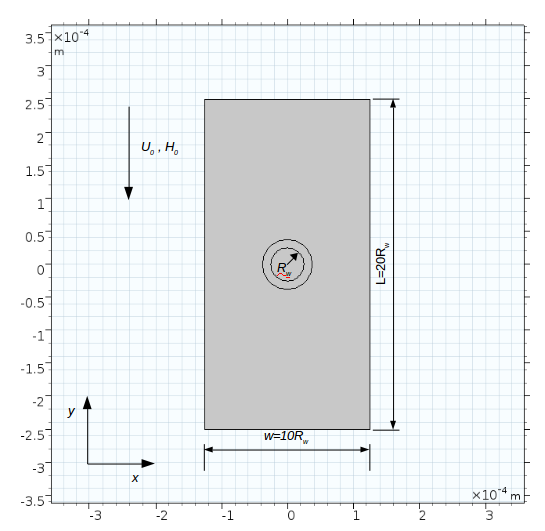
\includegraphics{figures/Comsol_single_wire_Geometry_long.png}
\caption[Single wire model geometry]{Single wire model geometry: the magnetic particles flow by a magnetized ferromagnetic cylinder with the radius $R_{w}$ in a rectangular channel with the length L=20$R_{w}$ and the width w=10$R_{w}$ in \textmu m; the uniform external field $H_{0}$ is applied parallel to the inlet flow velocity $u_{0}$; the retention of the particles is evaluated within the outer circular domain with a radius of 1.5$R_{w}$ and at the outlet of the channel}
\label{fig:geom_singlewire}
}
\end{figure}

For the generation of the mesh, the COMSOL method of physics-controlled meshing with free triangular elements, was applied. Hereby, information from the physics interface is used to set up an appropriate mesh sequence. As COMSOL mainly uses \gls{fem}, the accuracy of the solution is linked to the mesh size (for more information see Section\,\ref{subsec:FEM}). The smaller the mesh size the closer the approximation matches the exact solution of the \glspl{pde}. A decrease in element size, however, is always accompanied by an increase in computational effort. Therefore, a mesh refinement study was conducted with the goal to minimize the difference between the exact and the approximated solution, while still retaining reasonably low computing times. The residence time of the particles measured at the outflow was chosen as characteristic output parameter. As convergence criterion a deviation of the residence time smaller than 1.5\,\% from the current mesh to the next finer mesh was chosen. The different meshes tested in the refinement study are shown in Figure\,\ref{fig:Mesh_Ref} and the corresponding mesh size parameters are listed in Table\,\ref{table:Mesh_Ref}.  

\begin{figure}[h]
		%\centering
          \begin{subfigure}{0.24\textwidth}
                  \flushleft
                  \scalebox{0.3}{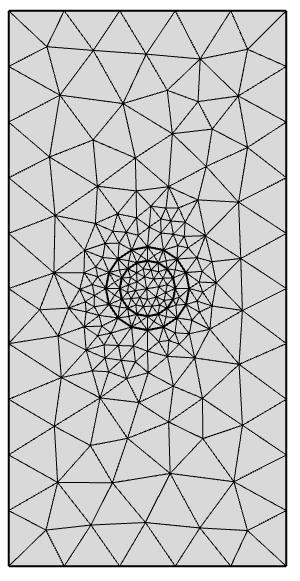
\includegraphics{figures/Comsol_single_wire_mesh_coarse.png}}
                  %\caption{Packing setup}\label{fig:Packing}
          \end{subfigure}\hfill	
	  \begin{subfigure}{0.24\textwidth}
                  %\flushleft
                  \scalebox{0.3}{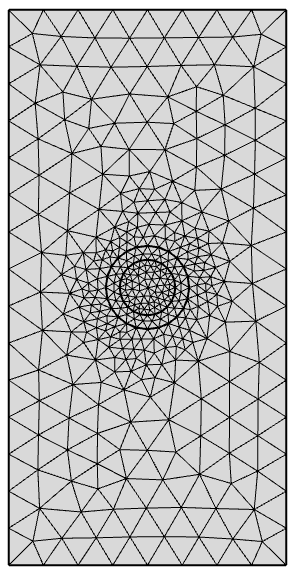
\includegraphics{figures/Comsol_single_wire_mesh_normal.png}}
                  %\caption{Packing setup}\label{fig:Packing}
          \end{subfigure}\hfill	
          \begin{subfigure}{0.24\textwidth}
                  %\flushright
                  \scalebox{0.3}{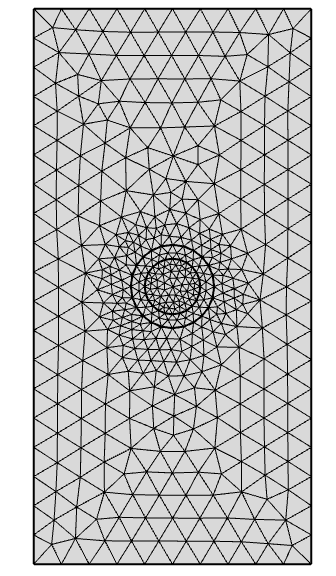
\includegraphics{figures/Comsol_single_wire_mesh_fine.png}}
                  %\caption{Packing setup}\label{fig:Packing}
          \end{subfigure}\hfill
        \begin{subfigure}{0.24\textwidth}
                \flushright
                \scalebox{0.3}{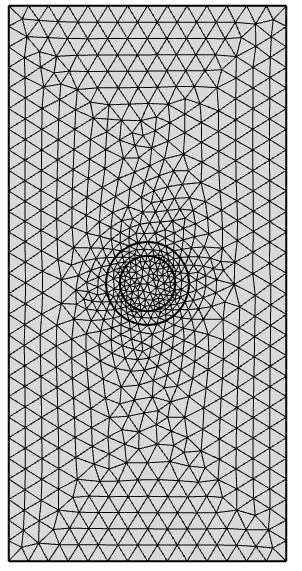
\includegraphics{figures/Comsol_single_wire_mesh_finer.png}}
                %\caption{Column}\label{fig:Column}
        \end{subfigure}
        \\
        
        \caption[Mesh refinement study]{The different meshes used in the mesh refinement study with the element-size from left to right: coarse, normal, fine, finer}
        \label{fig:Mesh_Ref}
  \end{figure}
 
 
\begin{table}[H]
\centering
\caption[Mesh size parameters]{Mesh size parameters used in the mesh refinement study}
\label{table:Mesh_Ref}
\begin{tabularx}{\textwidth}{XXXXX}\hline
Mesh &  Max. element size (\textmu m) & Min. element size (\textmu m) & Max. element growth rate & Curvature \newline factor \\
\hline\hline
coarse &  50.0 & 1.00 & 1.4 & 0.4 \\
normal &  33.5 & 0.15 & 1.3 & 0.3 \\
fine &  26.5 & 0.15 & 1.3 & 0.3 \\
finer &  18.5 & 0.0625 & 1.25 & 0.25 \\
\hline
\end{tabularx}
\end{table}

In addition to the two-dimensional single wire model, geometries with two and four wires were constructed. The setup and the meshing for those geometries are shown in Figure\,\ref{fig:Two_Four_Wires}. To assure comparability, the resulting mesh size from the mesh refinement study from the single wire model was chosen.  

\begin{figure}[h]
		%\centering
          \begin{subfigure}{0.24\textwidth}
                  \flushleft
                  \scalebox{0.3}{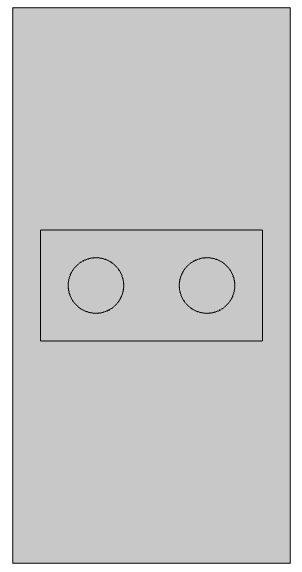
\includegraphics{figures/Comsol_two_wires_Geometry.png}}
                  %\caption{Packing setup}\label{fig:Packing}
          \end{subfigure}\hfill	
	  \begin{subfigure}{0.24\textwidth}
                  \flushleft
                  \scalebox{0.3}{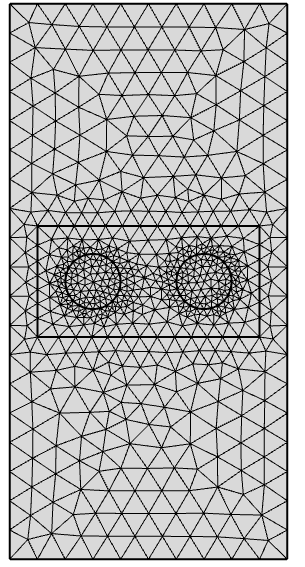
\includegraphics{figures/Comsol_two_wires_mesh_fine.png}}
                  %\caption{Packing setup}\label{fig:Packing}
          \end{subfigure}\hfill	
          \begin{subfigure}{0.24\textwidth}
                  \flushright
                  \scalebox{0.3}{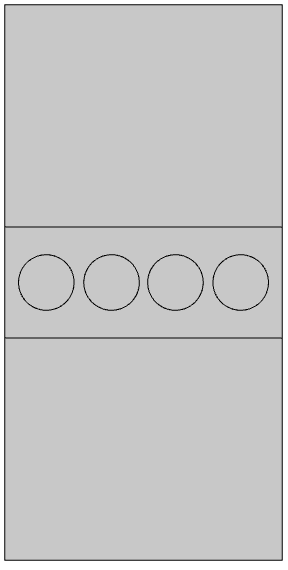
\includegraphics{figures/Comsol_four_wires_Geometry.png}}
                  %\caption{Packing setup}\label{fig:Packing}
          \end{subfigure}\hfill
        \begin{subfigure}{0.24\textwidth}
                \flushright
                \scalebox{0.3}{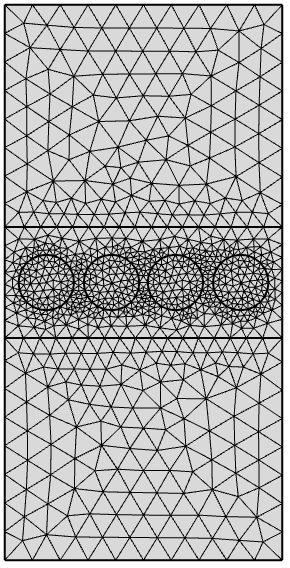
\includegraphics{figures/Comsol_four_wires_mesh_fine.png}}
                %\caption{Column}\label{fig:Column}
        \end{subfigure}
        \\
        
        \caption[Two cylinder and four cylinder setup]{Two cylinder setup geometry and fine mesh (left side) and four cylinder setup geometry and fine mesh (right side)}
        \label{fig:Two_Four_Wires}
  \end{figure}
  
For the two and four cylinder setup a channel with the same dimensions as shown in Figure\,\ref{fig:geom_singlewire} was used. For the two cylinder setup, the centers of the wires with the radius $R_{w}$ are located at at a distance of 2$R_{w}$ on the x-axis in each direction from the center of the channel. For the four cylinder setup, the cylinder centers are positioned at a distance of 3.5\,$R_{w}$ and 1.15\,$R_{w}$ respectively on each side of the channel center. For those two configurations, $R_{w}$ was fixed on 25\,\textmu m, while $R_{w}$ for the single wire model was also varied in the parameter studies described in Section\,\ref{subsec:Param_studies}. The retention of the magnetic nanoparticles was evaluated in the rectangle, drawn around the cylinders and at the outflow of the channel. To achieve a high resolution, the relative tolerance for all simulations was set to 0.001 for the stationary part and to 0.01 for the time-dependent part. In addition, the step width used by the \gls{bdf} solver was set to intermediate with an event tolerance of 0.01 and an initial step width of 0.001\,s. As sparse matrix solver the \gls{mumps} is used in the magnetic fields interface, while the \gls{pardiso} is used in the general form of the \gls{pde} interface (for more information on the linear system solvers see \cite{ComsolRefManual}).   

\subsection{Model parameters}
\label{subsec:Cond_param}

The parameters used in the simulation and their values are listed in Table\,\ref{table:param_mod}. Parameters that were varied in the parameter studies are not listed here but can be found in Section\,\ref{subsec:Param_studies}. For the material properties of the water and iron domain, values provided by the COMSOL material library were used.   

\begin{table}[h]
\centering
\caption[Model parameters]{Model parameters and natural constants used for the simulation}
\label{table:param_mod}
\begin{tabularx}{\textwidth}{XXX}\hline
Name & Description & Value \\
\hline\hline
$\rho_{w}$ & density of water &  997.1\,kg/m\textsuperscript{3}\\
$\mu_{w}$ & viscosity of water & 8.9$\cdotp$10\textsuperscript{-4}\,Pa$\cdotp$s\\
$T$ & temperature & 298.5\,K\\
$k_{b}$ & Boltzmann constant & 1.38064852$\cdotp$10\textsuperscript{-23}\,J/K\\
$\phi_{0}$ & initial volume fraction of magnetic particles & 1$\cdotp$10\textsuperscript{-4}\\
$\phi_{max}$ & maximum volume fraction of magnetic particles & 0.64\\
$\mu_{max}$ & maximum slurry viscosity & 10\textsuperscript{8}$\mu_{w}$\\
$x_{fmp}$ & weight fraction of of magnetite in magnetic particles & 0.9\\
$\rho_{pol}$ & density of polymer in particles & 950\,kg/m\textsuperscript{3}\\
$\rho_{fmp}$ & density of magnetite in the particles & 5050\,kg/m\textsuperscript{3}\\
$\chi_{fmp,0}$ & initial magnetic susceptibility of magnetite in the particles & 1000\\
$\chi_{w,0}$ & initial magnetic susceptibility of the iron wire & 1000\\
$M_{fmp,s}$ & saturation magnetization of magnetite in the particles & 4.55$\cdotp$10\textsuperscript{3}\,A/m\\
$M_{w,s}$ & saturation magnetization of the iron wire & 1735$\cdotp$10\textsuperscript{3}\,A/m\\
\hline
\end{tabularx}
\end{table}

\subsection{Model equations and boundary conditions}
\label{subsec:model_eq_BC}
In this section, a brief overview of the model equations and conditions is given, a more detailed model description can be found in \cite{choomphon2017simulation}. The external magnetic field was simulated with the magnetic fields interface of the AC/DC branch of COMSOL. It solves Maxwell's equations (see Section\,\ref{subsec:Maxwell}) formulated with the magnetic vector potential as described in Section\,\ref{subsec:Mag_pot}. In this model, the stationary equations \ref{eq:Ampere_stat} and \ref{eq:Pot_A} are solved for each domain together with the constitutive relation, described in Equation\,\ref{eq:B_tot} and the necessary material properties like $\mu_{r}$. The material properties are based on the assigned material for each domain. As initial condition, the magnetic vector potential is set to zero for all domains.  As boundary condition, magnetic insulation is applied to all four channel boundaries. The magnetic insulation boundary condition sets the tangential components of the magnetic potential to zero at the boundary ($\boldsymbol{n}\times\boldsymbol{A} = 0$). More information on the magnetic fields interface and corresponding equations and boundary conditions can be found in the COMSOL AC/DC module user guide \cite{ComsolACDC}. \newline
The fluid, flowing through the channel, consists of a slurry containing magnetic nanoparticles with the radius $R_{p}$ and water. The nanoparticles are composed out of magnetite and a diamagnetic polymer. The model was constructed in a way to include the effects of the particle accumulation on the wire both on the fluid flow and the magnetic field. To achieve this, the fluid viscosity is defined as a function of the magnetic particle concentration and the external forces are set to zero once the particles are collected, indicated by the maximum particle concentration. The velocity and the concentration of the slurry are described by the two-dimensional unsteady state Navier-Stokes equations for compressible fluid flow (see also Section\,\ref{subsec:Navier_Stokes}). The Equations \ref{eq:NS_part1} and \ref{eq:NS_part2} depict the Navier-Stokes equations for the solid (magnetic particles) and the liquid (water) fraction, respectively. 

%\begin{equation} 
\begin{multline} 
\rho_{p}\left(\frac{\partial}{\partial t}+(v_{s}\cdotp\nabla)\right)v_{s} = \\ \nabla\cdotp \begin{bmatrix} -\left(p+\frac{2}{3}\mu(\phi)\nabla\cdotp v_{s}\right)+2\mu(\phi)\frac{\partial v_{s,x}}{\partial x} & \mu(\phi)\left(\frac{\partial v_{s,y}}{\partial x}+\frac{\partial v_{s,x}}{\partial y}\right) \\ \mu(\phi)\left(\frac{\partial v_{s,y}}{\partial x}+\frac{\partial v_{s,x}}{\partial y}\right)  &  -\left(p+\frac{2}{3}\mu(\phi)\nabla\cdotp v_{s}\right)+2\mu(\phi)\frac{\partial v_{s,y}}{\partial y}\end{bmatrix}\\ + \frac{(F_{m}+F_{d}+F_{b})}{V_{p}}\Phi(\phi)
\label{eq:NS_part1}
% %\begin{bmatrix} 1&2\\3&4\end{bmatrix}
\end{multline}
%\label{eq:NS_part}
%\end{equation}

\begin{multline} 
\rho_{w}\left(\frac{\partial}{\partial t}+(v_{l}\cdotp\nabla)\right)v_{l} = \\ \nabla\cdotp \begin{bmatrix} -\left(p+\frac{2}{3}\mu(\phi)\nabla\cdotp v_{l}\right)+2\mu(\phi)\frac{\partial v_{l,x}}{\partial x} & \mu(\phi)\left(\frac{\partial v_{l,y}}{\partial x}+\frac{\partial v_{l,x}}{\partial y}\right) \\ \mu(\phi)\left(\frac{\partial v_{l,y}}{\partial x}+\frac{\partial v_{s,x}}{\partial y}\right)  &  -\left(p+\frac{2}{3}\mu(\phi)\nabla\cdotp v_{s}\right)+2\mu(\phi)\frac{\partial v_{l,y}}{\partial y}\end{bmatrix}\\ - \frac{\phi F_{d}}{(1-\phi)V_{p}}
\label{eq:NS_part2}
% %\begin{bmatrix} 1&2\\3&4\end{bmatrix}
\end{multline}

$v_{s}=(v_{s,x},v_{s,y})$ denotes the velocity of the solid, while  $v_{l}=(v_{l,x},v_{l,y})$ is the velocity of the liquid. $\phi$ is the particle volume fraction in the fluid, $\mu(\phi)$ is the dynamic viscosity of the fluid, that is dependent on $\phi$ and $\Phi(\phi)$ is a constraint function that approaches a value of zero when $\phi$ approaches its maximum value which leads to the cancellation of all forces once the particles are collected. The continuity equations for the liquid and the particle phase can be written as follows:  

\begin{equation}
\frac{d\rho_{s}}{d t}+\nabla\cdotp(\rho_{s}V_{s})=0
\label{eq:Conti_p}
\end{equation}

\begin{equation}
\frac{d\rho_{l}}{d t}+\nabla\cdotp(\rho_{l}V_{l})=0
\label{eq:Conti_l}
\end{equation}

where the solid and liquid densities can be defined as $\rho_{s}=\phi\rho_{p}$ and $\rho_{l}=(1-\phi)\rho_{w}$ with $\rho_{p}$ as the density of a single particle and $\rho_{w}$ as the density of water. The equations are implemented in the general form \gls{pde} interface.\\
As the magnetic particles are assumed to be in the nanometer range (for values of $R_{p}$ see Section\,\ref{subsec:Param_studies}) only magnetic, hydrodynamic and diffusion forces are considered and the gravitational force is neglected. For calculation of the forces the Equations \ref{eq:mag_force}, \ref{eq:drag_force} and \ref{eq:diff_force} are modified in the following way:  

\begin{equation}
\label{eq:mag_force_model}
\centering
\boldsymbol{F}_{m} = \frac{1}{2}\mu_{0}V_{p}\omega_{fmp}\nabla(\boldsymbol{M}_{fmp}\boldsymbol{H_{f}})
\end{equation}

\begin{equation}
\label{eq:drag_force_model}
\centering
\boldsymbol{F}_{d} = 6\pi\mu(\phi)R_{p}(\boldsymbol{v}_{l}-\boldsymbol{v}_{s})
\end{equation}

\begin{equation}
\label{eq:diff_force_model}
\centering
\boldsymbol{F}_{b}= 
                 \begin{cases}
                    -k_{B}T\frac{\nabla\phi}{\phi} & \text{if}\ \phi>0 \\
                    0 & \text{if}\ \phi=0
                 \end{cases}
\end{equation}

where $\omega_{fmp}$ is the volume fraction of the magnetite in the magnetic particles, $M_{fmp}$ is the magnetization of the particles and $H_{f}$ is the local magnetic field around the wire, which is defined by $H_{f}=H_{0}-\nabla\varphi_{2}$. Herein $\varphi_{2}$ is the magnetic potential in the liquid domain and $H_{0}$ the externally applied uniform magnetic field. The induced magnetization in the wire  by $H_{0}$ is described by the following Equation.


\begin{equation}
\label{eq:mag_wire}
\centering
\boldsymbol{M}_{w}= 
                 \begin{cases}
                    \frac{2\chi_{w,0}}{2+\chi_{w,0}}H_{0} & \text{if}\ \frac{2\chi_{w,0}}{2+\chi_{w,0}}H_{0}<M_{w,s} \\
                    \frac{M_{w,s}}{H_{0}}H_{0} & \text{if}\ \frac{2\chi_{w,0}}{2+\chi_{w,0}}H_{0}\geq M_{w,s} \\
                 \end{cases}
\end{equation}

No-slip and no-flux boundary conditions are applied at the wire's surface, while periodic boundary conditions or Dirichlet boundary conditions with a fixed flow velocity are applied at the channel walls. The boundray conditions on the channel walls were selected in order to model a chromatographic column with far more than just one cylinder in a channel. A Dirichlet boundary condition of $p$=0 was set at the outflow to simulate an open-boundary flow with an ambient pressure of zero and an inflow velocity $u_{0}$ was set at the inflow.


\subsection{Parameter studies}
\label{subsec:Param_studies} 
In order to evaluate the influence of the different parameters on the retention of the magnetic nanoparticles, parameter studies were conducted. For the parameter studies, the following parameters were varied: the magnetic flux density of the external field $B_{0}$ in mT, the particle radius $R_{p}$ in nm, the radius of the wire $R_{w}$ in \textmu m and the inflow velocity of the slurry $u_{0}$ in \textmu m/s. For the two and four cylinder models $R_{w}$ was held constant. The design of the parameter studies is shown in Table\,\ref{table:param_study} with the corresponding value ranges of the varied parameters. 

\begin{table}[H]
\centering
\caption[Parameter study]{Parameter study design: with the model description where sw=single wire, tw=two wires, fw=four wires and the corresponding constant parameter values and value ranges}
\label{table:param_study}
\begin{tabularx}{\textwidth}{XXXXX}\hline
Model & $B_{0}$ in mT & $R_{p}$ in nm & $R_{w}$ in \textmu m & $u_{0}$ in \textmu m/s\\
\hline\hline
sw, tw, fw & 0-35 & 30 & 25 & 200\\
sw, tw, fw & 0-32.5 & 20-150 & 25 & 200\\
sw, tw, fw & 0-32.5 & 30 & 25 & 150-400\\
sw & 0-32.5 & 30 & 5-45 & 200\\
\hline
\end{tabularx}
\end{table}

The flow and magnetic conditions were simulated for 10\,s for each case, where the nanoparticles were introduced in a constant concentration into the domain between 0.1s and 0.2s after the start of the simulation. As characteristic parameter the residence time of the particles is determined in the secondary circle around the wire and at the outflow (see Equation\,\ref{eq:residence_time}). For the two and four cylinder setup, the residence time of the particles is determined within the rectangle around the wires and at the outflow of the channel. The residence time is then normalized by the division with the residence time at 0\,mT and otherwise unchanged parameters. 

\begin{equation}
\label{eq:residence_time}
\centering
\tau = \frac{\phi(t)}{\int_{0}^{\infty}\phi(t)dt}
\end{equation}
% \subsection{Model validation/verification}
% \label{subsec:model_val}
% Benchmark problem flow around a cylinder (Schaefer and Turek)
% Comparison of drag coefficients
% 
% Comparison with analytical solution of magnetic field around a wire

\section{Experimental setup}
\label{sec:Exp_setup}
For the validation of the simulation results and as a proof of principle of the operational concept several experimental runs were designed. In order to evaluate the retention of a magnetic nanoparticle suspension within a magnetizable packed bed a chromatographic system was used (see Section\,\ref{subsec:chrom_sys}). The nanoparticle suspension is characterized in Section\,\ref{subsec:Mag_nanoparticles} and the matrix materials in Section\,\ref{subsec:Matrix_mat}. Furthermore an overview of the conducted experiments is given in Section\,\ref{subsec:Exp_Pro}. In Section\,\ref{subsec:ana_met} the analytical methods and in Section\,\ref{subsec:Eval} the evaluation methods are discussed.    


\subsection{Magnetic nanoparticle suspension}
\label{subsec:Mag_nanoparticles}
The experiments were conducted with two different types of magnetic nanoparticles. For the experiments in Section\,\ref{subsec:Exp_Pro} a nanoparticle suspension from Chemagen (Chemagen Biopolymer Technology, Baesweiler, Germany) was used. The magnetic nanoparticles from Chemagen consist of a core of magnetite coated with \gls{pva}. A stock solution with a concentration of 73\,g/l was used. In order to minimize aggregation, the stock solution was put into an ultrasonic bath for 20 minutes before use. Then the stock solution was diluted 1:100 with 20\,mM sodium phosphate buffer with a pH of 6.5 and filterd through a filter with a pore size of 450\,nm. 
In addition,  plain nanomag\textsuperscript{\textregistered}-D-spio particles from micromod (Micromod Partikeltechnologie GmbH, Rostock, Germany) with mean diameters of 20\,nm and 100\,nm were utilized for the experiments. The micormod nanoparticles are composed of iron oxid domains coated by an unmodified dextran surface. The stock solution with a concentration of 25\,g/l was also diluted 1:100 with a 20\,mM phosphate buffer. In additon a 1:1 mixture of the two nanoparticle sizes was used. In contrast to the Chemagen nanoparticles, the micromod particles required no additional ultrasonic treatment and filtration in order to remove aggregates.     

\subsection{Matrix material}
\label{subsec:Matrix_mat}
For the packed bed three different matrix materials were evaluated. In Table\,\ref{table:mat_material} the three magnetizable materials and their corresponding composition are listed.    

\begin{table}[H]
\centering
\caption{Matrix materials and their composition}
\label{table:mat_material}
%\begin{tabular}{llllllll}\hline
\begin{tabularx}{\textwidth}{XXXXXXXX}\hline
\multirow{2}{*}{name} & \multirow{2}{*}{charge/lot} & \multirow{2}{*}{producer} & \multicolumn{5}{c}{composition in \%}  \\
& & & Fe & C & Cr & Ni & Mo \\
\hline\hline
SRA-150 & W140401E & H.C. Stark & 83.95 & 0.16 & 12.5  & & \\
LSM Fe-4021 & 154001 & m4p & 85.37 & 0.23 & 12.8 & & \\
TruForm\textsuperscript{TM} 316-3 & 15 & Praxair & 68.1 & 0.017 & 16.66 &11.31& 2.66\\
\hline
\end{tabularx}
\end{table}

The matrix material SRA-150 was already used in preceding experiments by \cite{AndreMaster}. In order to achieve a narrow particle-size distribution the SRA-150 particles were sieved with a mesh size of 25\,\textmu m and 20\,\textmu m respectively. In addition the matrix materials TruForm 316-3 and were chosen due to its spherical structure and material composition. 
As a negative control \gls{pmma} particles from microParticles GmbH were used. 

\subsection{Column packing}
\label{subsec:col_pack}
As chromatographic column a Omnifit\textsuperscript{\textregistered} BenchMark\textsuperscript{TM} Microbore chromatography column (Omnifit Labware, Diba Industries, Danbury, USA) was used. The borosilicate glass column has a column length of 10\,mm, a column inside diameter of 3\,mm and a total volume capacity of 0.7\,ml. On both sides of the column endpieces with pre-assembled frits were used to hold back the matrix material. For the experiments with \gls{pmma} and SRA-150 \gls{ptfe} frits with a pore size of 25\,\textmu m were used. In addition punched out polycarbonate filters with a pore size of 2\,\textmu m and an O-ring were added to the inlet and outlet of the column. For the experiments with the TruForm 316-3 matrix material \gls{ptfe} frits with a pore size of 5\,\textmu m were used, no additional filters were necessary. \\   
For the column packing a slurry consisting of the matrix material and either ultra-pure water for \gls{pmma} or a 20\,\% Ethanol suspension for SRA-150 and TruForm 316-3 was used. Ethanol was used in order to simplify the packing of the column due to the reduced surface tension. To remove impurities and achieve a narrower particle size distribution the \gls{pmma} matrix material was first mixed with the solvent and left to settle for several minutes. After sedimentation the supernatant was removed and replaced by fresh solvent. This procedure was repeated till the supernatant was a clear fluid. For the other two matrix materials instead of sedimentation a magnet was held to the outside of the falcon to seperate the magnetizable particles from the supernatant.\\   
A CETONI neMESYS syringe pump (CETONI GmbH, Korbussen, Germany), controlled by a QmixElements software, was connected to bottom of the column via a tube (see Figure\,\ref{fig:Packing_Setup_Column}). With this set-up a negative pressure was generated within the column into which the matrix material slurry is drawn from the column inlet. The slurry was added to the column inlet by a pipette. Once the column was completely filled, the syringe pump was disconnected and the endpiece with the corresponding frit or filter was placed on top of the column. Then the packed bed within the column was compressed with the help of an \gls{fplc}-system (described in Section\,\ref{subsec:chrom_sys}) to eliminate possible cavities. Afterwards the column was again connected to the syring pump and the resulting void at the top filled with new matrix material. This procedure was repeated until no further compression of the matrix material could be observed. The column and the syringe pump are shown in Figure\,\ref{fig:Packing_Setup_Column}.
%%%%%%%%%%%%%%%%%%%%Include Figure of setup and column%%%%%%%%%%%%%%%%%%%%%%%%%%%%%%%%%%%%%%%%%%%%%%%%%%%%%%%%%%%%%%%%%%%%%%%%%%%%%%%%%%%%%%%%%%%%%%%%%%%%%%%%%%%%%%

\begin{figure}[h]
		%\centering
          \begin{subfigure}{0.49\textwidth}
                  \flushleft
                  \scalebox{0.12}{\includegraphics{figures/Column_Packing_All_numbers.pdf}}
                  %\caption{Packing setup}\label{fig:Packing}
          \end{subfigure}\hfill
        \begin{subfigure}{0.49\textwidth}
                \flushright
                \scalebox{0.0545}{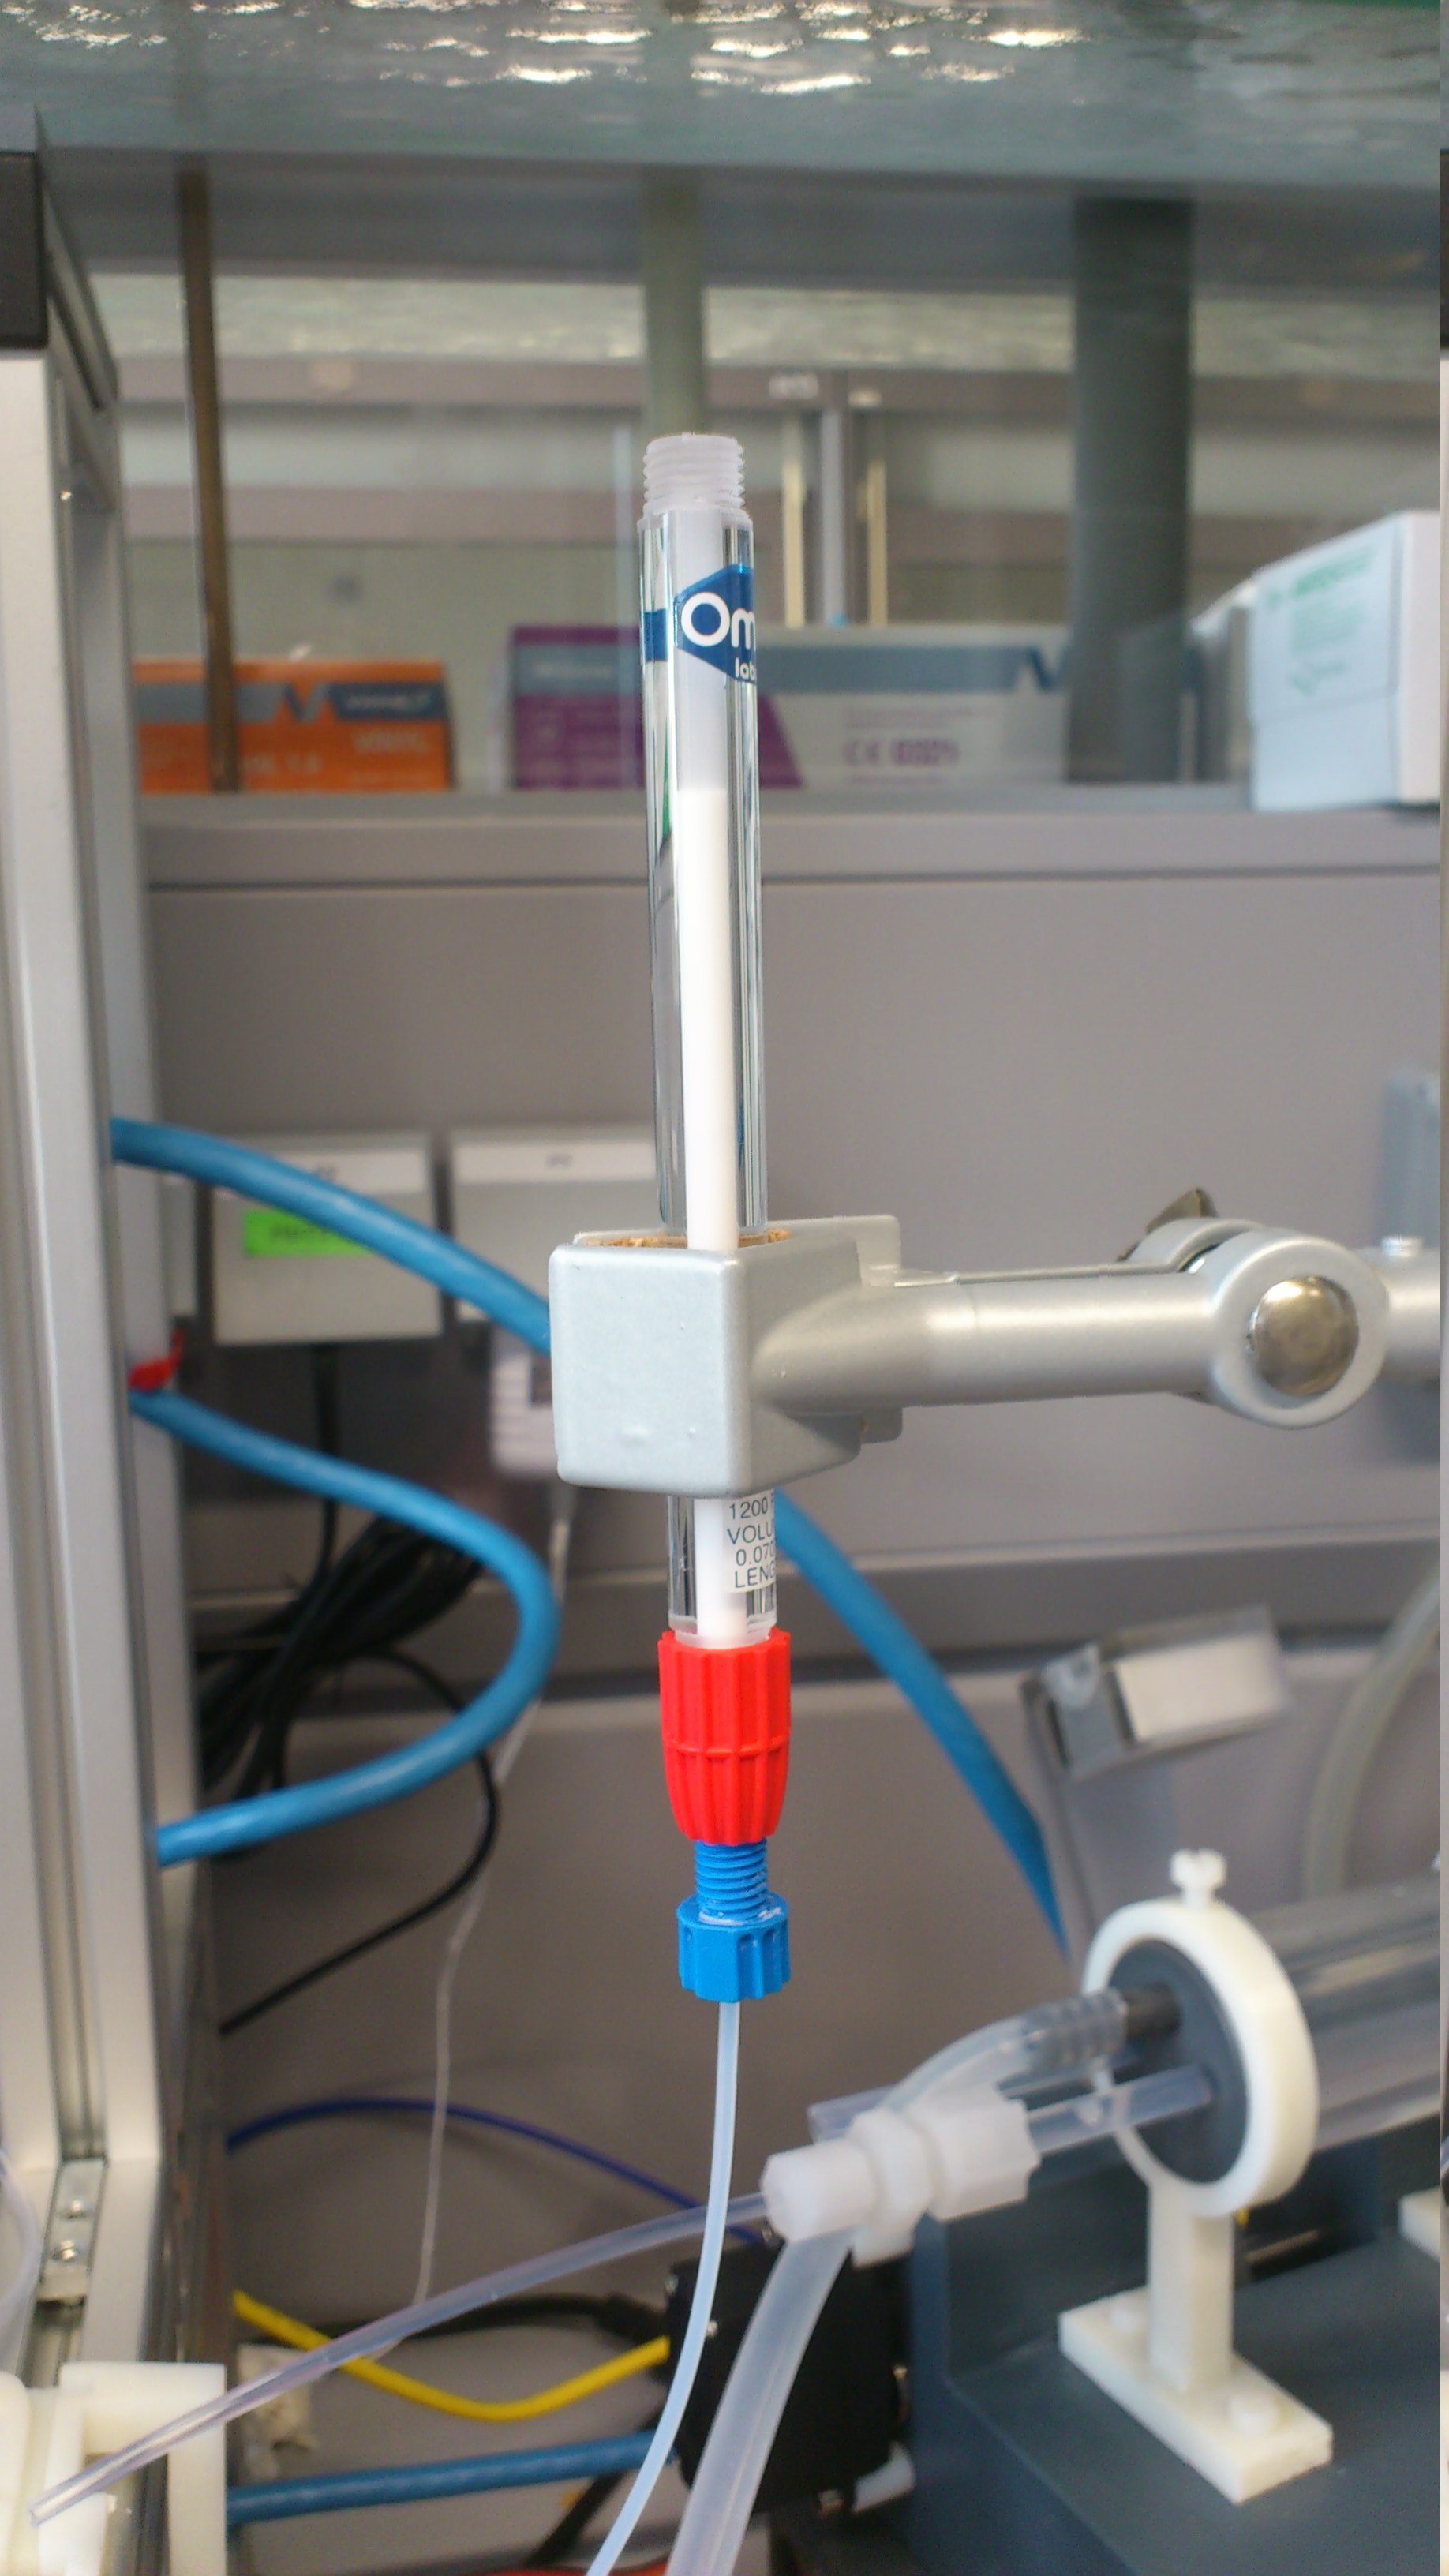
\includegraphics{figures/Column_Packing_Column.jpg}}
                %\caption{Column}\label{fig:Column}
        \end{subfigure}
        \\
        
        \caption[Column packing setup]{Column packing setup; left side: CETONI neMESYS control station (1), column (2) and syring pump (3); right side: Column packed with \gls{pmma} matrix material }
        \label{fig:Packing_Setup_Column}
  \end{figure}  




% \begin{figure}[H]
% \centering
% 
% \scalebox{0.30}{\includegraphics{Bioreactor_real.png}}
% \caption{Photobioreactor with 37 light cylinders for the cultivation of microalgae
% \label{fig: Bioreactor_real}
% }
% \end{figure} 
% 
% \begin{figure}[h]
% 		\centering
%           \begin{subfigure}{0.49\textwidth}
%                   \flushleft
%                   \scalebox{0.30}{\includegraphics{Bioreactor_Geometry.png}}
%                   \caption{Lateral view of the photobioreactor}\label{fig:Bioreactor_Geometry}
%           \end{subfigure}
%         \begin{subfigure}{0.49\textwidth}
%                 \flushright
%                 \scalebox{0.32}{\includegraphics{Bioreactor_cross_section.png}}
%                 \caption{Cross section of the photobioreactor}\label{fig:Bioreactor_cross_section}
%         \end{subfigure}
%         \\
%         
%         \caption{Structure of the photobioreactor with 37 light cylinders}
%         \label{fig:Bioreactor}
%   \end{figure}  


\subsection{Chromatographic system}
\label{subsec:chrom_sys}
For the compression of the packed bed within the column and the execution of the retention experiments an Äkta purifier \gls{fplc}-system from GE Healthcare (Buckinghamshire, England) was used. For all connections tubings with an inner diameter of 0.25\,mm (PEEK tubings blue, GE Healtcare Bio-Sciences AB, Uppsala, Sweden) were used to achieve high resolution peaks. The samples were injected via a sample loop with a total volume of 100\,\textmu m. The experiments were conducted with ultra-pure water as solvent and a constant flow rate. An inline UV flow cell was used to continuously measure the absorbance of the liquid at a wavelength of 280 nm and to transmit the data to the computer. A conductivity flow cell was used to measure the conductivity of the passing solution. For further analysis the samples were collected by a fraction collector. The regulation of the \gls{fplc}-system and the analysis of the transmitted data was realized by the software Unicorn. The experimental setup is shown in Figure\,\ref{fig:  }.
%%%%%%%%%%%%%%%Include Figure of ÄKta and Fraction collector%%%%%%%%%%%%%%%%%%%%%

\begin{figure}[H]
		\centering
          \begin{subfigure}{0.49\textwidth}
                  \flushleft
                  \scalebox{0.05}{\includegraphics{figures/Column_Packing_All_numbers.pdf}}
                  \caption{\textbf{Change photo with photo of ÄKTA system}}\label{fig:Bioreactor_Geometry}
          \end{subfigure}
        \begin{subfigure}{0.49\textwidth}
                \flushright
                \scalebox{0.09}{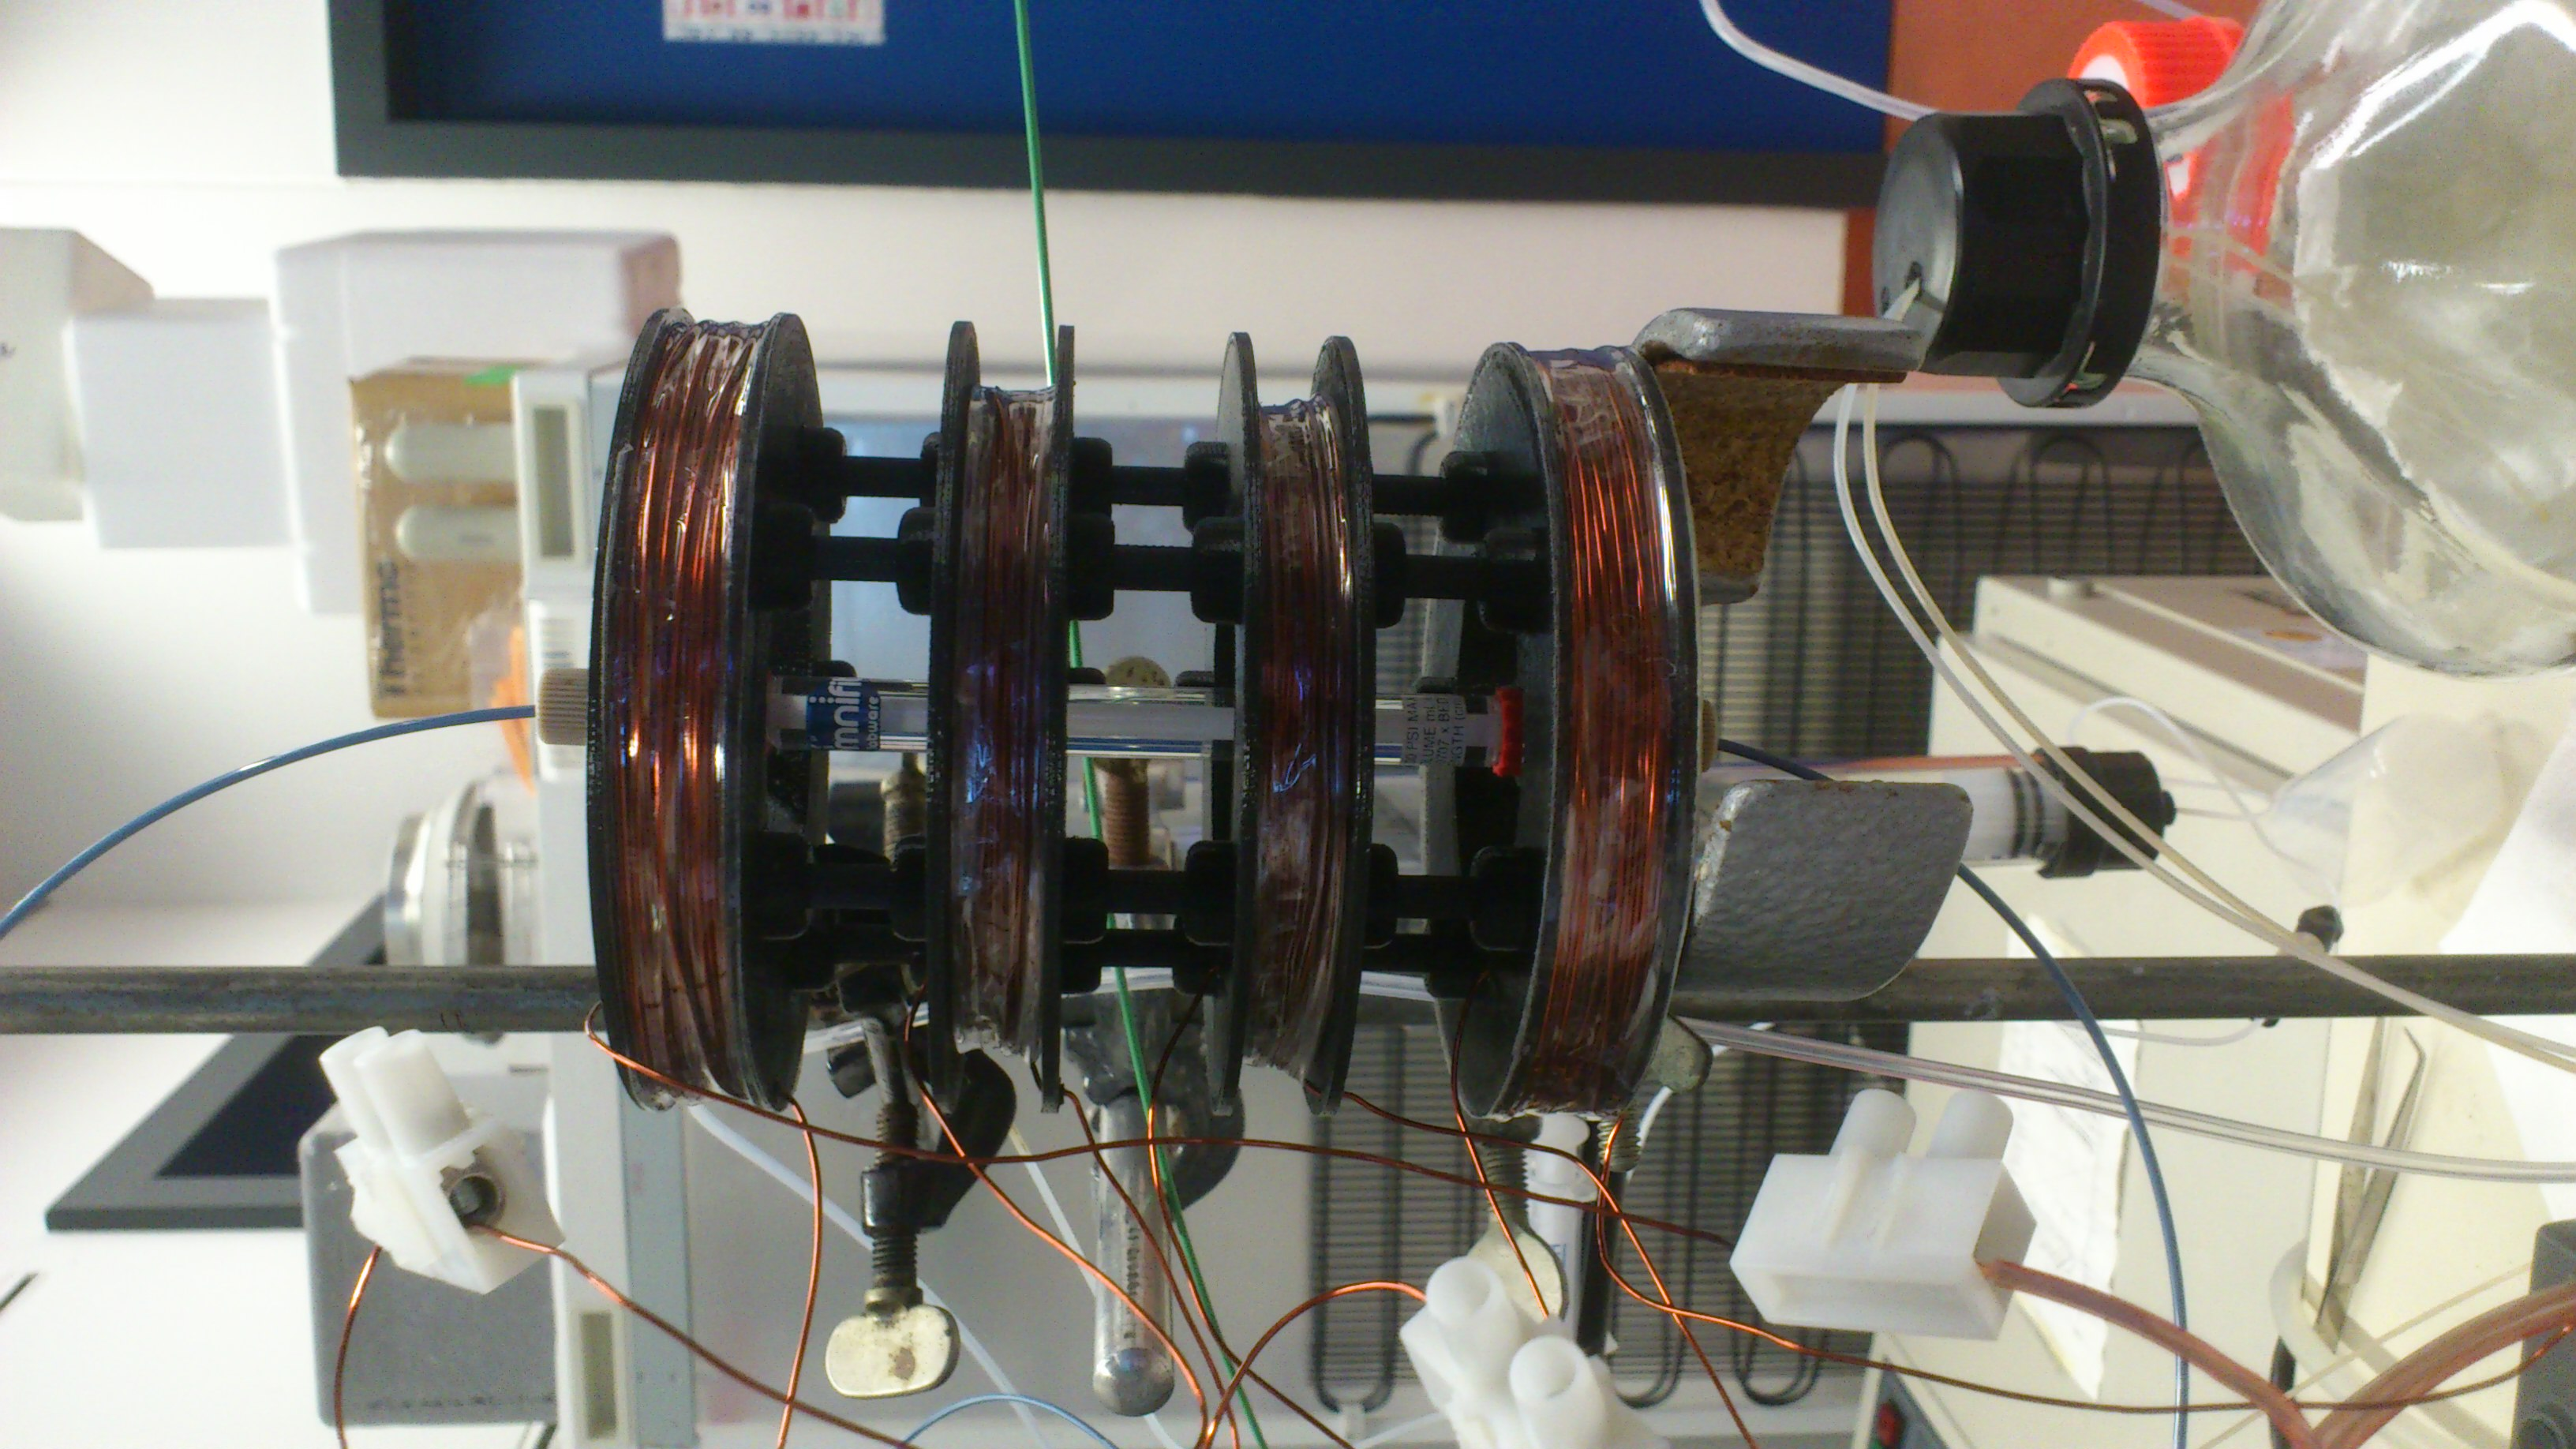
\includegraphics{figures/Helmholtz_Coil_Column.jpg}}
                \caption{Chromatographic column within the Helmholtz coil}\label{fig:Bioreactor_cross_section}
        \end{subfigure}
        \\
        
        \caption{Chromatographic system and the used Helmholtz coil}
        \label{fig:Bioreactor}
  \end{figure}  


\subsubsection{Chromatographic system with a Helmholtz coil}
\label{subsubsec:helm_coil}
For all experiments a Helmholtz coil was used to create a stable homogeneous magnetic field around the column. The Helmholtz coil consists of an assembly of four coils with the distance D between each other. The whole length of the four coils was based on the length of the column. The other calculated dimensions of the Helmholtz coil can be found in Table\,\ref{table:Helmholtz_coil} (more detailed information on the dimensioning of Helmholtz coils can be found in \cite{wotruba1968verbesserung,wotruba1969massive,heller1955erzeugung}). The Helmholtz coil was constructed so that for a current of 2\,A a magnetic field of 14\,mT was created. The coil was also designed to be used in an ultrasonic bath. The technical drawing for the construction of the used Helmholtz coil is shown in Figure\,\ref{fig:Helmholtz_coil}\\  
The Helmholtz coil was included in the chromatographic system as shown in Figure\,\ref{fig: ???}. The coil was connected to a power amplifier (19 Z/500, FG Elektronik) to increase the electrical signal and therefore the magnetic field within the coil. The square wave signals were generated by a function generator (Rigol DG1022, RIGOL Technologies Inc., Beijng, China). The adjustment of the magnetic flux density was achieved by the regulation of the electric current measured with a digital multimeter(MY64, Mastech Group LLC., CA, USA).   

\begin{table}[H]
\centering
\caption[Dimensions of the Helmholtz coil]{Calculated dimensions of the Helmholtz coil}
\label{table:Helmholtz_coil}
\begin{tabular}{ll}\hline
Parameter &  Value \\
\hline\hline
 number of turns in each coil n & 300 \\
 filling factor F & 0.73\\
 diameter of copper wire $d_{D}$ & 0.70\,mm\\
 coil depth & 10\,cm\\
 distance between coils D & 3.3\,cm \\
 inner radius $R_{i}$ & 3.0\,cm\\ 
 outer radius $R_{a}$ & 4.58\,cm\\
 mean/average radius $R_{m}$ & 3.79\,cm\\
 \hline
\end{tabular}
\end{table}


\begin{figure}[H]
		\centering
          \begin{subfigure}{0.49\textwidth}
                  \flushleft
                  \scalebox{0.40}{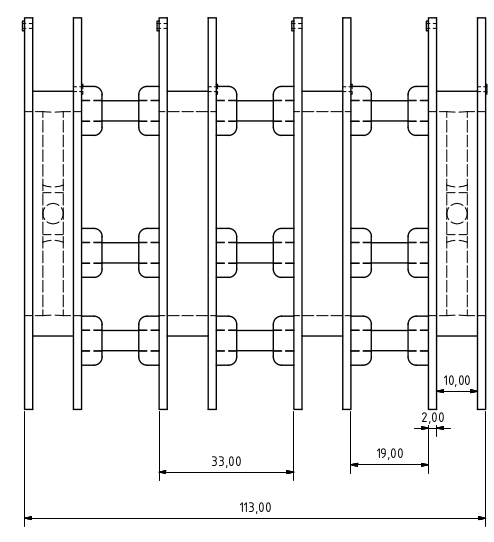
\includegraphics{figures/Helmholtz_Coil_Full.png}}
                  \caption{Side view of the Helmholtz coil}\label{fig:Coil_Full}
          \end{subfigure}
        \begin{subfigure}{0.49\textwidth}
                \flushright
                \scalebox{0.5}{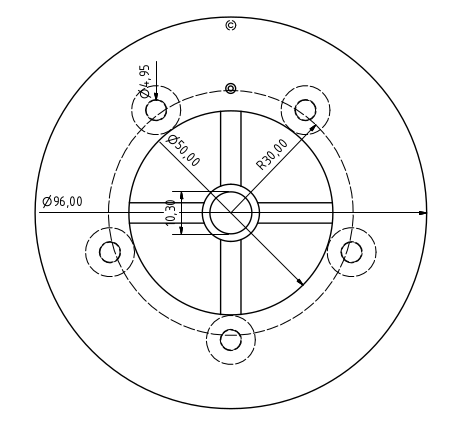
\includegraphics{figures/Helmholtz_Coil_Top.png}}
                \caption{Top view of the Helmholtz coil}\label{fig:Coil_Top}
        \end{subfigure}
        \\
        
        \caption[Technical drawing of the Helmholtz coil]{Technical drawing of the Helmholtz coil with length specifications in mm }
        \label{fig:Helmholtz_coil}
  \end{figure}  

\subsection{Experimental procedures}
\label{subsec:Exp_Pro}
All experiments were programmed and regulated using the control software Unicorn 5.20 (GE Healthcare Life Sciences). Before each injection the column was washed with 2\,ml of ultra-pure water to remove remaining nanoparticles from the previous injection. To achieve comparability and reproducibility all experiments were conducted with the same method, except for the fractionation and saturation experiments ,for which a separate method was created. All experiments were done in triple determination. \\
Before each experiment series the quality of the column packing was controlled. For this purpose a one percent acetone solution was injected and the asymmetry of the  resulting UV peak analyzed. For a packing with \gls{pmma} an asymmetry between 1 and 2 and for a packing with the TruForm particles an asymmetry between 1 and 1.5 was considered tolerable. For deviating asymmetry values the column was emptied and repacked. After each experiment series the column was demagnetized with the help of a degaussing coil (Entmagnetisierer EM-60, MAGNET-PHYSIK Dr. Steingroever GmbH, Cologne, Germany). Afterwards the column was washed until no significant change in the UV signal was perceived anymore. To clean the filters of the column and reduce the back pressure a change between up- and down-flow was applied while washing when necessary. Once a pressure of 50\,bar was reached the filters were replaced. The blocked filters were regenerated by storing them for 24 hours in oxcalic acid with a concentration of 250\,g/l on a stirrer plate with the lowest heating level.

\subsubsection{Flow rate optimization}
\label{subsubsec:Flow_rate}
In a first step the flow rate was optimized for each matrix material. For this purpose flow rates of 0.1\,ml/min, 0.2\,ml/min and 0.5\,ml/min were tested. The nanoparticle suspension was injected with a volume of 100\,\textmu l and the above mentioned method (see Section\,\ref{subsec:Exp_Pro}) run with the corresponding flow rates. The resulting UV peaks were analyzed for their asymmetry and reproducibility. Also the comparability with the results from \cite{AndreMaster} was taken into consideration.  

\subsubsection{Retention of magnetic nanoparticle suspension}
\label{subsubsec:Ret_nanopart_method}
The main objective of this experiments was to asses the retention of the magnetic nanoparticles through a magnetized packed bed. The magnetization of the packed bed was achieved by the Helmholtz coil described in Section\,\ref{subsubsec:helm_coil}. The homogeneous magnetic field within the coil was created by a power amplifier connected to a function generator, which generated an alternating current with a square wave signal. The power amplifier was used to change the electric signal and thereby vary the magnetic flux density. For all experiments a flow rate of 0.5\,ml/min and magnetic flux densities between 0\,mT and 17\,mT were used. \\
The magnetic field could be influenced by the variation of the frequency, duty cycle and amplitude. A constant magnetic field was produced by setting the high and low state to the closest values possible. The smallest difference achievable with the used function generator was 4\,mV. Therefore a high level value of 400\,mV and a low level value of 396\,mV was used to approximate a direct current (see Figure\,\ref{fig:waveform}). To investigate the impact of an alternating magnetic field the low level was set to -\,400\,mV wereas the high level stayed at 400\,mV. To simulate a magnetic field being turned on and off a low level value of 0\,mV was chosen. For the matrix material \gls{pmma} all described variations were applied with the frequencies 100\,mHz and 1000\,mHz . For the matrix material Stark and TruFrom only the constant and on/off fields with frequencies of 100\,mHz, 500\,mHz and 1000\,mHz were tested. The duty cycle, the ratio of the high period to the total period of the square wave, was set to 50\,\% for all experiments. An exception was an experiment with the TruForm particles were the off phase was reduced to 20\,\%.

\begin{figure}[h]
\centering

\scalebox{0.60}{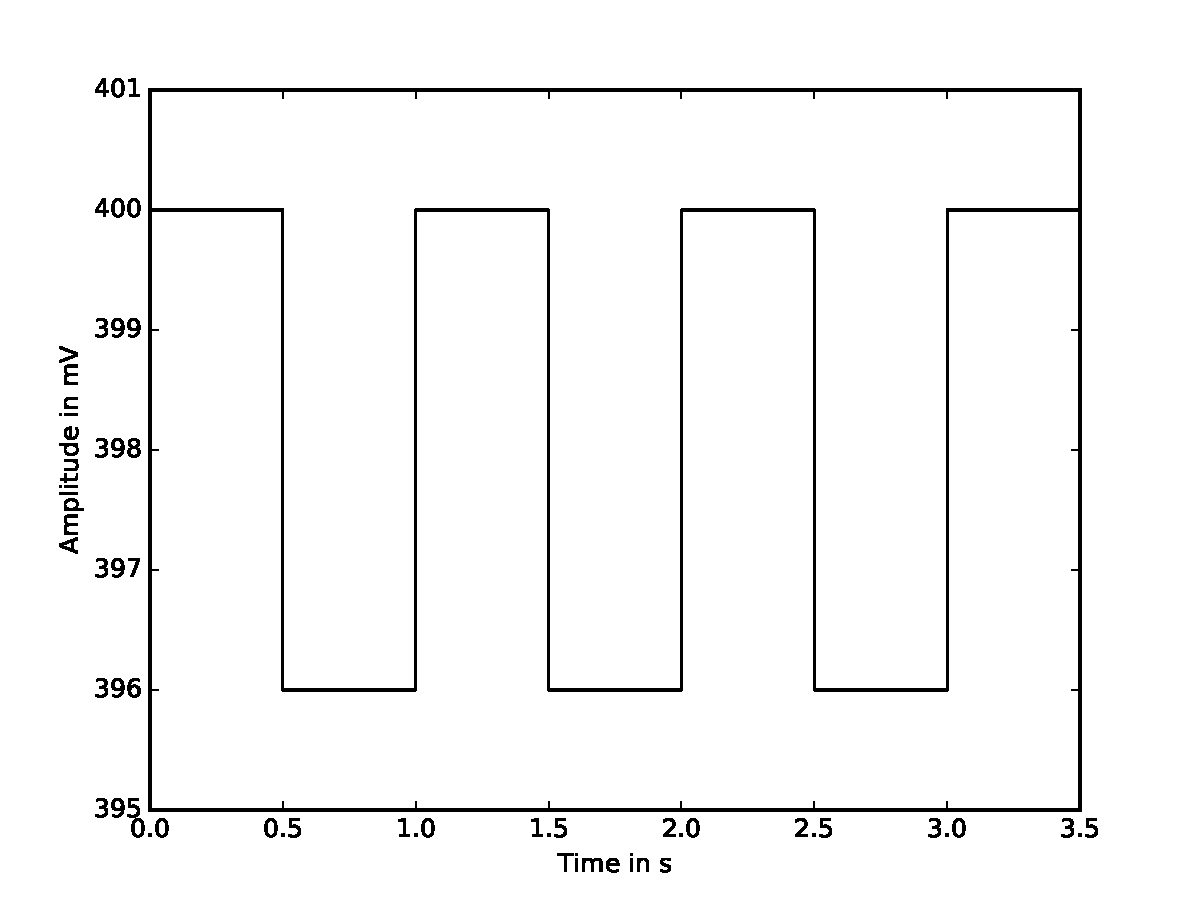
\includegraphics{figures/waveform.pdf}}
\caption[Example of a square wave signal]{Example of a square wave signal used for the generation of a constant magnetic field with a frequency of 1\,Hz, a high level of 400\,mV and a low level of 396\,mV
\label{fig:waveform}
}
\end{figure}


In addition saturation experiments were conducted with the TruForm material. For those experiments the column was first washed with 1\,ml and no magnetic field, next the sample solution was injected and the constant magnetic field was turned on. The magnetic field was held till the column was washed with 2\,ml. The cycle was repeated till no further change in the UV peak could be observed. The experiment was conducted twice, once with an used and once with a new filter. A magnetic flux density of 17\,mT was used for the saturation experiments.\\
In order to evaluate the influence of the nanoparticle concentration on the retention behaviour, Chemagen nanoparticel suspension was diluted 1:100, 1:150 and 1:200. The dilutions were tested with TruForm matrix material and a constant magnetic field. The micromod nanoparticle suspensions were also only used for experiments with the TruForm matrix material and a constant magnetic field.\\
For further analysis the third peak of each triple determination was fractionated and collected in 1.5\,ml Eppendorf tubes. A Unicorn method was written to start the fractionation as soon as an increase in the UV signal was detected. As fraction volume 200\,\textmu l was chosen. The fractionation was stopped as soon as the UV signal sank below 0.1\,mAu. 
 

%%%%%%%%%Tabelle mit Parametern ?%%%%%%%%%%%%%%%%%%%%%%%%%%%%%%%%%%%%%%%%%%%%%%%%%
 

\subsection{Analytical methods}
\label{subsec:ana_met}
 For the characterization of the matrix materials and the nanoparticle suspensions several different analytical methods were used. The particle size distribution was determined either by dynamic light scattering, light micrsocope or under the \gls{esem} described in Sections \ref{subsubsec:part_dist_meas}, \ref{subsubsec:light_mic} and \ref{subsubsec:ESEM}. The method for the determination of the magnetic properties is described in Section\,\ref{subsubsec:Mag_char}. For characterization of the magnetic field within the Helmholtz coil a Hall effect sensor was used (see Section\,\ref{subsubsec:Hall_eff}).   
 
 
\subsubsection{Measurement of particle size distributions}
\label{subsubsec:part_dist_meas}
For the determination of the particle size distribution two different measurement devices were used. The matrix materials were analyzed with an CIS 100-S particle sizer (Galai, Migdal Haemek, Israel). The measurement system combines two analytical techniques, namely laser obstruction time analysis and dynamic image analysis to analyze both the size distribution and shape factors of the sample. For the laser obstruction time measurement a helium-neon laser with a wavelength of 600\,nm rotates with a constant frequency and interacts with particles in the sample solution. Each scanned particle temporarily blocks the path of the laser beam to the corresponding photo diode, which registers the time of transition. The obstruction time in combination with the frequency is then related to the particle diameter \cite{neis1997particle}. Additionally dynamic image analysis is used to determine the particle shape parameters. With this combination spherical and non-spherical particles in a range between 0.1\,\textmu m to 3,600\,\textmu m can be measured. For each sample a three-fold determination was conducted, with a length of 60\,s for each measurement cycle. In addition the reproducibility of the measurement was verified by the measurement software. As sample preparation a spatula tip of the matrix material was mixed with 2\,ml of ultra-pure water. Of this suspension 1500\,\textmu l were filled into a cuvette. If necessary the sample was further diluted with ultra-pure water. During the measurement period the suspension was continuously mixed with a pipette (Eppendortf Research \textsuperscript{\textregistered} plus (blue), Eppendorf AG, Hamburg, Germany) to ensure homogeneity. \\
\\
For the determination of the particle size distributions of the magnetic nanoparticle suspensions and the collected nanoparticle fractions (see Section\,\ref{subsubsec:Ret_nanopart_method}) a Zetasizer Nano ZSP (Malvern Instruments, Malvern, England) was used. The nanoparticle stock suspensions were diluted 1:100 in ultra-pure water, while for the fractions no further dilution was necessary. The Chemagen nanoparticle solution was measured in filtered and unfiltered form (see Section\,\ref{subsec:Mag_nanoparticles}), whereas the micromod particles were not filtered at all. For each measurement 50\,\textmu l of the sample was pipetted into a quarz cuvette and put into the Zetasizer. For all samples a triple determination was conducted. The size measurement was performed by dynamic light scattering. Particles scatter the light from a helium-neon laser with a wavelength of 633\,nm creating a fluctuation in the detected scattering intensity over time. This fluctuation is due to the Brownian motion, which leads to diffusion of particles at a speed related to their size and temperature. From the intensity changes a correlation function is generated from which the diffusion coefficient is deducted. The particle size distribution is then calculated with the Stokes-Einstein equation (see Equation\,\ref{eq:eq:Stokes_Einstein}) \cite{berne2000dynamic}. Particle sizes could be measured in the range of 0.3\,nm to 10\,\textmu m \cite{Zetasizer}. For the evaluation only particles in the nanometer size range were considered. In order to reduce the influence of contaminations, either leaked matrix material or dust, within the samples, all particles with a size of over 1\,\textmu m were not included in the size distributions.

\subsubsection{Environmental scanning electron microscope}
\label{subsubsec:ESEM}
The particle shape, size and surface properties were characterized with an \gls{esem} (XL 30-FEG, Philips, Amsterdam, Netherlands). \gls{esem} is a procedure in which uncoated samples can be examined with an electron beam. The samples to be analyzed were placed within the sample chamber. Then a vacuum was applied reaching pressures between 130\,Pa and 1300\,Pa. An electron beam is focused on the sample which leads to the ejection of secondary electrons from the sample surface. These secondary electrons are then accelerated towards the electric field of an detector. The detected signal is converted into an image of the sample. With this method it is possible to magnify the samples by a factor of 50 up to 5100 \cite{danilatos1993introduction}.     
\gls{esem} measurements were used for the characterization of the TruForm matrix material. As sample preparation a defined quantity of the matrix material was put on a sample holder. No further sample preparation was needed.

\subsubsection{Light microscope}
\label{subsubsec:light_mic}
The characterization of the \gls{pmma} matrix material was conducted with the help of a VHX-5000 digital microscope system (Keyence, Osaka, Japan). A 500 frames per second camera captures image data with different focus positions and generates high resolution images on an attached monitor. By variation of the shutter speed the resolution and contrast are further increased. In addition the optimal wavelength to generate clear images is automatically selected \cite{VHX5000}. For the measurement the matrix material was suspended in ultra-pure water. A few drops of the suspension were placed on a slide and put onto the object stage. The magnification was slowly increased until a high resolution image was aquired. By measuring the distance from two neighbouring pixel on the screen dimension measurements were possible. With this method the mean diameter of the measured matrix particles was determined.    


\subsubsection{Concentration determination of the nanoparticle suspension}
\label{subsubsec:Conc_MF}
For the determination of the Chemagen nanoparticle concentration 200\,\textmu l of the particle suspension was filled into an HPLC vial. All measurements were conducted in triple determination. Before filling the empty weight of the vials was determined with a MC5 microbalance (Sartorius, Göttingen, Germany). The vials were dried for 24 hours at \SI{60}{\celsius} in a drying cabinet (drying cabinet ULE 500, Memmert GmbH, Schwabach, Germany). The vials were allowed to cool in a desiccator for 20 minutes and then weighed again. From the difference between the current and the empty weight the mass of the magnetic nanoparticles could be calculated. With the calculated mass and the used suspension volume the concentration could be determined.  


\subsubsection{Magnetization determination of the matrix materials and nanoparticle suspension}
\label{subsubsec:Mag_char}
The characterization of the magnetic properties of the matrix materials was performed with an \gls{agm} (Micromag 2900, Princeton Measurments Corp, Princeton, USA). As sample preparation a defined amount of matrix material was given onto a strip of adhesive tape and hermetically sealed with another piece of tape. The sample was then placed onto a cantilevered rod including a piezoelectric element, magnetized by a dc field and overlaid by an oscillating magnetic field gradient. Through the  oscillating magnetic field gradient the sample experiences an alternating force  which is proportional to the magnitude of the field gradient and the magnetic moment of the sample. This force deflects the sample rod within the magnetic field which leads to a voltage output of the piezoelectric element. With a variation of the alternating magnetic field strength the voltage signals can be converted into a magnetization curve \cite{flanders1988alternating}. The magnetization within the magnetization curve was normalized with the mass of the used sample. Before the actual measurements, the \gls{agm} was calibrated with a nickel standard. From the hysteresis loop the magnetic properties of the materials could be extracted. On all samples a threefold determination was performed.    

\subsubsection{Analysis of the magnetic flux density}
\label{subsubsec:Hall_eff}
The magnetic flux density within the Helmholtz coil was measured with a Hall effect sensor (FH 31/4, MAGNET-PHYSIK Dr. Steingroever GmbH, Cologne, Germany). The Hall effect sensor consists of a thin rectangular p-type semiconductor material on which a constant current is applied. When the sensor is placed in a magnetic field perpendicular to the current the electrons are deflected towars one edge of the sensor. The result is a potential difference that develops between the upper and lower edge of the conductor which is referred to as the Hall voltage. The Hall voltage is proportional to the applied current and the magnetic flux density \cite{svoboda2004magnetic}.\\%%%%%V=-(I*B)/(e*rho*t) 
The magnetic flux density of the Helmholtz coil was measured for different currents in six different positions along the symmetry axis. The resulting flux density was then compared to the calculated values for the Helmholtz coil (see Section\,\ref{subsubsec:helm_coil}). 


\subsection{Evaluation methods}
\label{subsec:Eval}
For the evaluation of both, the particle size distribution and the retention experiments, evaluation routines were written in python. Wherever possible the same evaluation methods as in \cite{AndreMaster} were applied to ensure comparability. 

\subsubsection{Graphical evaluation}
\label{subsubsec:Graph_eval}
In order to compare the results from the particle size distribution measurements, the D-values D10, D50 and D90 were determined. D50 is defined as the diameter where half of the particles are smaller than this value. Likewise 10\,\% of the population lie below the value from D10 and 90\,\% below the value of D90 \cite{merkus2009particle}. The cumulative distribution is  approximated by a least squares polynomial fit, where the solution minimizes the squared error E (see Equation\,\ref{eq:polyfit_er}) for the equations shown in \ref{eq:polyfit_eq}.  

\begin{equation}
\label{eq:polyfit_er}
\centering
E = \sum_{j=0}^{k}\vert p(x_{j})-y_{j}\vert^{2}
\end{equation}

\begin{equation}
\label{eq:polyfit_eq}
\centering
\begin{split}
x[0]^{n}p[0] + ... + x[0]p[n-1] + p[n] = y[0] \\
x[1]^{n}p[0] + ... + x[1]p[n-1] + p[n] = y[1]  \\
... \\ 
x[k]^{n}p[0] + ... + x[k]p[n-1] + p[n] = y[k]
\end{split}
\end{equation}

Where $p$ represents the polynomial coefficients, $n$ the degree of the polynomial, $y$ the y-coordinates and $x$ the x-coordinates of the sample points. The coefficient matrix of the coefficient $p$ is called Vandermonde matrix \cite{bjorck1970solution}. With this fit the D-values were calculated. 
%%%%%%%%%%%%%%%%Add Number distribution%%%%%%%%%%%%%%%%%%%%%%%%%%%%%%%%%%%%%

\subsubsection{Mathematical evaluation}
\label{subsubsec:Math_eval}
For the evaluation of the retention experiments with the magnetic nanoparticle suspensions the UV signal from the \gls{fplc}-system was used. The influence of the magnetic field was determined by a comparison of the UV peak area and retention with the retention and area of a control peak with no magnetic field applied. The area of the peak (see Equation\,\ref{eq:area}) provides information about the particles bound in the packed bed at a certain magnetic field strength.    

\begin{equation}
\label{eq:area}
\centering
area = \sum_{j=1}^{N}[(x_{i+1}-x_{i})(\frac{y_{i+1}+y_{i}}{2})]
\end{equation}

The first term on the right side of Equation\,\ref{eq:area} depicts an infinitely small interval of the volume which has flown through the column in ml, while the second term describes the average of the UV signal in mAU within the limits of x. The results were normalized by dividing the area of a peak with an applied magnetic field by the area of a standard peak without the influence of ante magnetic field. \\

%%%%%%%%%Check this find better description%%%%%%%%%%%%%%%%%%%%%%%%%%%%%%%%

The equations for the calculation of the retention of the nanoparticles are shown in the following: 

\begin{equation}
\label{eq:ret_sum}
\centering
k = k_{s} = \sum_{j=1}^{N}[(x_{i+1}-x_{i})(\frac{y_{i+1}+y_{i}}{2})(\frac{x_{i+1}+x_{i}}{2})]
\end{equation}

\begin{equation}
\label{eq:ret_comp}
\centering
retention = \frac{k}{k_{s}}
\end{equation}

In order to evaluate the influence of the retention the average of volume $(x_{i+1}+x_{i})/2$ within the infinitely small interval of $x_{i+1}-x_{i}$ was added to the area. The retention $k$ of a field under magnetic influence was also normalized by the division with the retention $k_{s}$ of a standard peak.   

%%%%%%%%%%%%%%%%%%%%%%%%%%%%%%%%%%%%%%%%%%%%%%%%%%
%%%%%%%%%%%%%%%%%%%%%%%%%%%%%%%%%%%%%%%%%%%%%%%%%%
%%%%%%%%%%%%%%%%%Results%%%%%%%%%%%%%%%%%%%%%%%%%%
%%%%%%%%%%%%%%%%%%%%%%%%%%%%%%%%%%%%%%%%%%%%%%%%%%
%%%%%%%%%%%%%%%%%%%%%%%%%%%%%%%%%%%%%%%%%%%%%%%%%%


\chapter{Results and Discussion}
\label{chap:chap_res}
In this chapter the results from the model parameter studies are presented and discussed in Section\,\ref{sec:sim_res}. Furthermore the the experimental results are shown and compared with the the simulation results (see Section\,\ref{sec:exp_res}). 

\section{Simulation results}
\label{sec:sim_res}
The model of the retention of nanoparticles by magnetized cylindrical wires, described in Section\,\ref{sec:Model_setup}, was run and evaluated as described in Section\,\ref{subsec:Param_studies}. In order to validate the model, the results are compared to analytical and published simulated solutions for the magnetic field and the flow around a cylinder. In Section\,\ref{subsec:Param_res} the results from the parameter studies and their influence on the nanoparticle retention are presented and discussed.  

\subsection{Mesh refinement study}
\label{subsec:mesh_ref}
As the accuracy of \gls{fem} models is strongly dependent on the mesh size, a mesh refinement study was performed. The model was also used to perform parameter studies, therefore it was also important to limit the increase in computation time to an acceptable value, that still allowed the simulation of several model runs in a  relatively short time period. The convergence of the tracking parameter residence time and the computation time for the individual runs of the parameter study are shown in Table\,\ref{table:Mesh_Ref_res}. The specifications for the different mesh sizes can be found in Table\,\ref{table:Mesh_Ref}. The deviation of the residence time of 1.04\,\% between the fine and the finer mesh element size lies below the beforehand specified convergence criterion of a deviation smaller than 1.5\,\%. In addition, a considerable increase of 228\,\% in computation time from 27\,s to 74\,s could be observed between those two meshes. Hence the fine mesh size was chosen for all further simulations. 

\begin{table}[H]
\centering
\caption[Mesh refinement study results]{Mesh refinement study results with tracked residence time for convergence determination and the computation time for each run}
\label{table:Mesh_Ref_res}
\begin{tabularx}{\textwidth}{XXXX}
\hline
Mesh & Residence time in s & Deviation in \% & Computation time in s\\
\hline\hline
coarse &  2.01 & -  & 11\\
normal & 1.95 & 3.07 & 20\\
fine &  1.85 & 5.16 & 27 \\
finer &  1.83 & 1.04 & 74\\
\hline
\end{tabularx}
\end{table}

\subsection{Model validation}
\label{subsec:mod_val}

The model validation was conducted by the comparison of the simulation results with analytical and other model solutions, as well as experimental data.
The simulated magnetic field around a single wire is shown in Figure\,\ref{fig:sw_mag_field}. 

\begin{figure}[H]
		%\centering
            \begin{subfigure}{0.49\textwidth}
                  \flushleft
                  \scalebox{0.39}{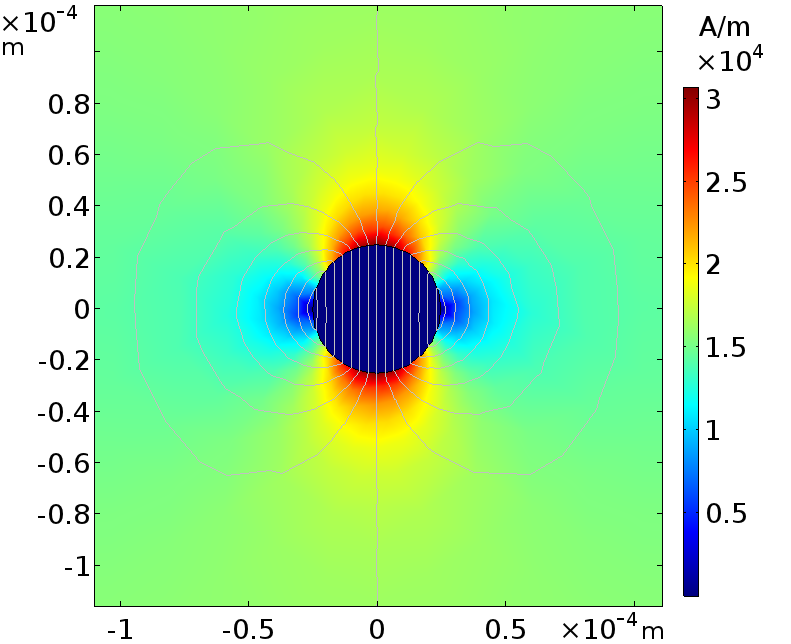
\includegraphics{figures/Hfield_around_single_wire_close.png}}
                  \caption{Simulated magnetic field intensity in A/m and magnetic field lines (gray lines) in the vicinity of a magnetized ferromagnetic wire}\label{fig:sw_mag_field}
          \end{subfigure}\hfill
        \begin{subfigure}{0.49\textwidth}
                \flushright
                \scalebox{0.39}{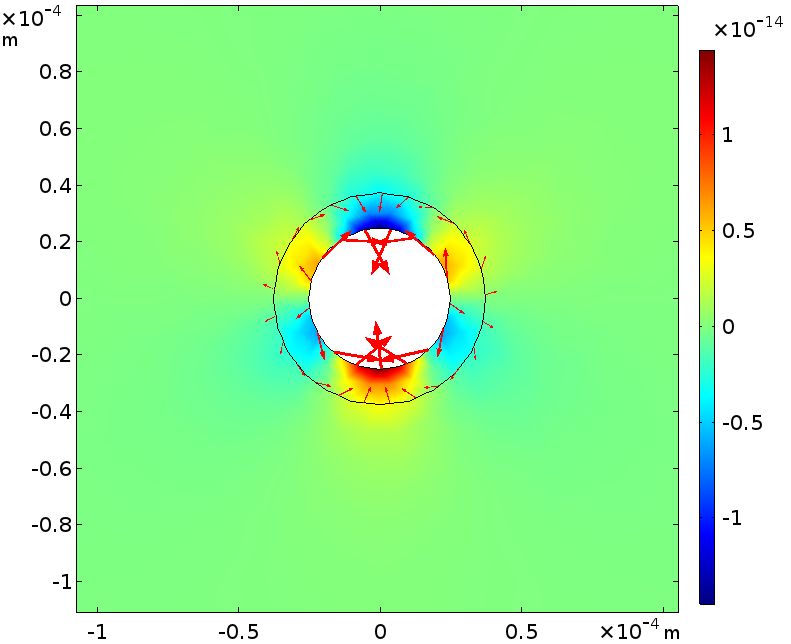
\includegraphics{figures/mag_force_wire.png}}
                \caption{Simulated magnetic field gradient in y-direction in A/m\textsuperscript{2} and the magnetic force $F_{m}$ depicted as red arrows their lenght beeing proportional to the magnitude of the force}\label{fig:mag_force_sw}
        \end{subfigure}
        \\
        
        \caption[Simulated magnetic field around a single wire]{Simulated magnetic field around a single wire in the longitudinal arrangement for an external magnetic field of 20\,mT}
        \label{fig:sw_fm_mag_field}
  \end{figure}

% \begin{figure}[H]
% \centering
% 
% \scalebox{0.4}{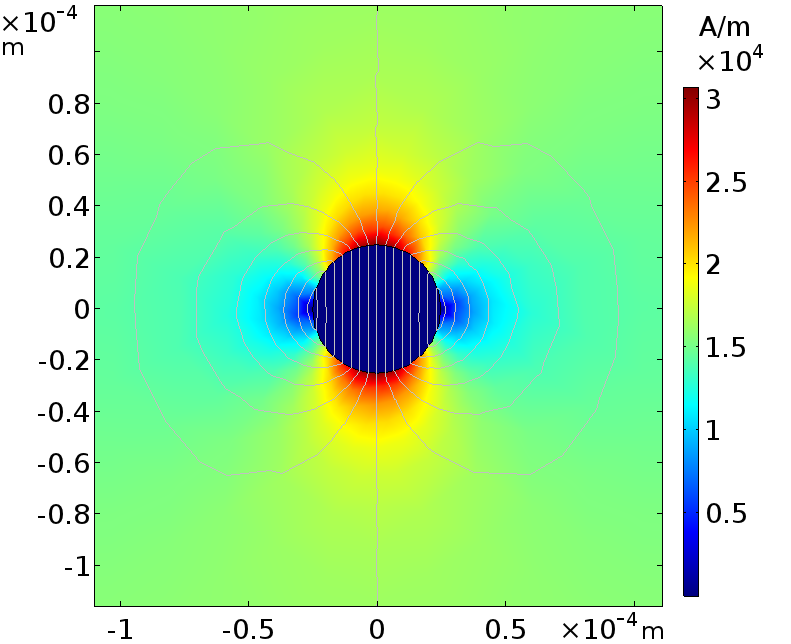
\includegraphics{figures/Hfield_around_single_wire_close.png}}
% \caption[Simulated magnetic field intensity around a single wire]{Contour plot of the simulated magnetic field intensity in A/m and magnetic field lines (gray lines) in the vicinity of a magnetized ferromagnetic wire in the longitudinal arrangement for an external magnetic field of 20\,mT \textbf{add figures with larger font}
% \label{fig:Hfield_sw}
% }
% \end{figure}

The colors indicate the magnetic field strength where maxima/minima in the direction/perpendicular to the magnetic field can be observed. A maximum value of 3.07$\cdotp$10\textsuperscript{4}\,A/m and a minimum of 3.58\,A/m are detected for the magnetic field intensity. This indicates that the field is attractive on the top and bottom of the wire i.e. a positive magnetic field gradient prevails, while it is repulsive on both wire sides, i.e. a negative field gradient develops. These attractive and repulsive magentic forces are visualized in Figure\,\ref{fig:mag_force_sw}, where the color indicates the magnitude of the magnetic field gradient in the y-direction and the arrows indicate the direction and magnitude of the magnetic force $F_{m}$. The magnetic field intensity around a circular wire simulated by Lindner et al. \cite{lindner2013simulation} exhibits very similar positions for the minima and maxima of the magnetic field strength in regard to the field direction and also a very similar overall distribution of the magnetic field intensity (see Figure\,\ref{fig:mag_field_nirschl}). The magnetic field lines depicted in Figure\,\ref{fig:sw_mag_field} also match with the experimental visualization of the magnetic field lines in Figure\,\ref{fig:mag_field_hale}. The magnetic field lines exhibit a very similar pattern in both cases, as in the two-dimensional case no distinction between wire and sphere can be made. The field lines are denser in the close vicinity of the wire reflecting the high magnetic field strength, while the field lines become less dense with the diminishing field strength at a distance from the wire. As the simulation is in good accordance with both the experimental and the simulated data, the model was deemed adequate for the simulation of the magnetic field.  

\begin{figure}[H]
		\centering
            \begin{subfigure}{0.49\textwidth}
                  \flushleft
                  \scalebox{0.372}{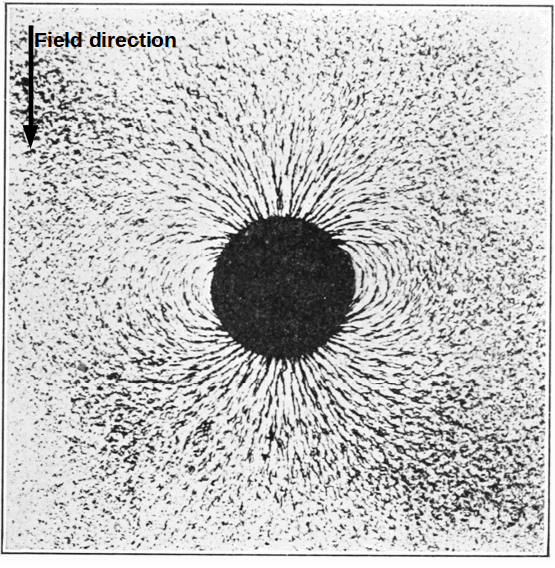
\includegraphics{figures/Force_flow_of_a_magnetized_steel_sphere_mod.png}}
                  \caption{Magnetic field lines around a magnetized steel sphere visualized by iron fillings sprinkled across a glass plate \cite{hale1913magnets}}
                  \label{fig:mag_field_hale}
          \end{subfigure}\hfill
        \begin{subfigure}{0.49\textwidth}
                \flushright
                \scalebox{0.198}{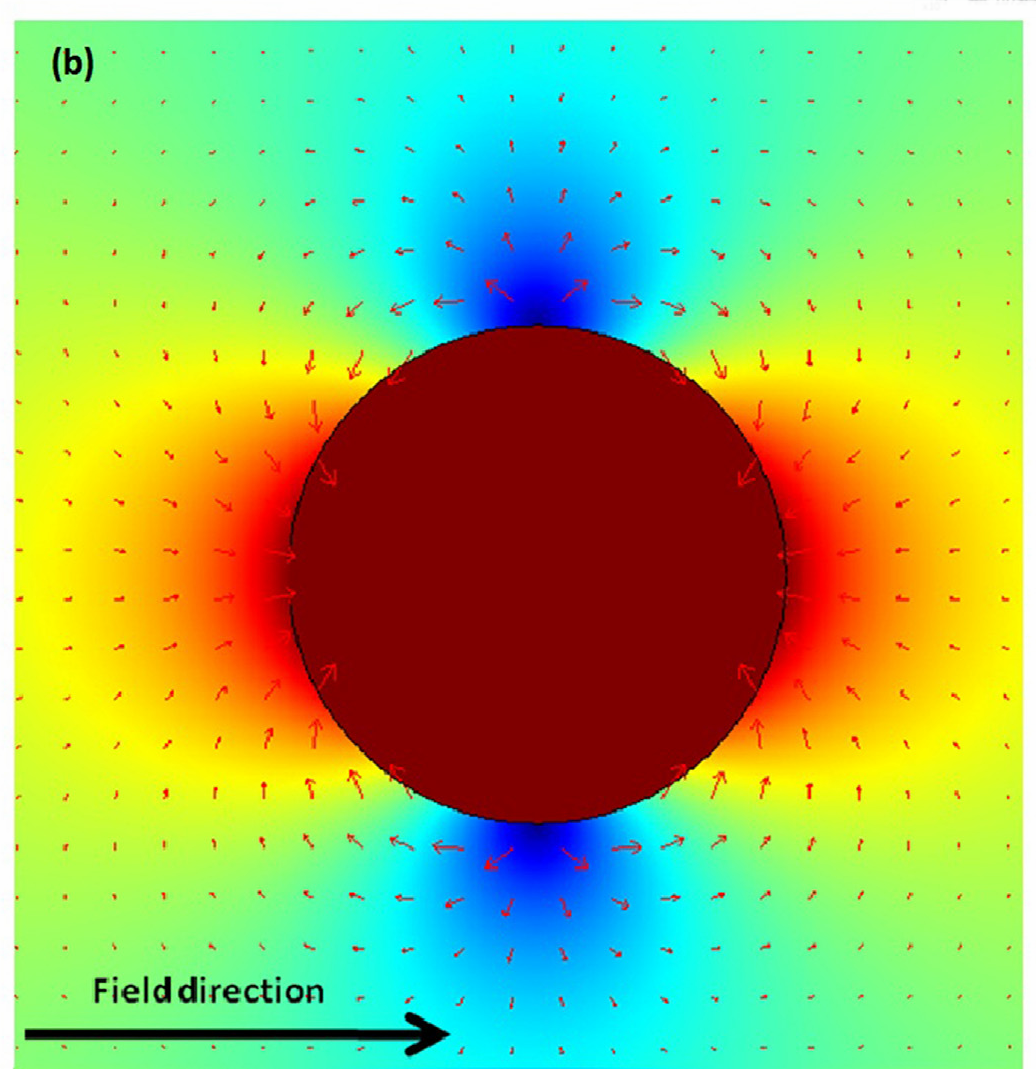
\includegraphics{figures/H_field_magntized_sphere_Nirschl.png}}
                \caption{Simulated magnetic field intensity and field gradient around a cylindrical wire \cite{lindner2013simulation}}\label{fig:mag_field_nirschl}
        \end{subfigure}
        \\
        
        \caption[Magnetic field around a magnetized sphere and wire]{Magnetic field around a magnetized sphere and wire (2-D)}
        \label{fig:esem_prax}
  \end{figure}

 
Figure\,\ref{fig:creep_flow_sw} shows the simulated streamlines around a single wire for an inlet velocity of 20\,mm/s with no-slip boundary conditions at the wires surface and constant velocity at the channel walls. The image depicts the typical streamlines, that also develop in flow experiments (see Figure\,\ref{fig:creep_1}) past a circular cylinder for low Reynolds numbers.  A streamline is a path traced out by a massless particle as it moves with the flow. It can be seen that the steady-state flow is completely symmetrical to both the y- and the x-axis. At a distance from the wire the flow is unidirectional and uniform. On both sides of the cylinder the flow speed increases in consistence with the Bernoulli equation, which leads to a lower pressure in those regions. The vertical streamlines at the cylinder center clearly suggest the stagnation points where velocity is zero at the upstream and downstream sides of the cylinder. Overall the simulated flow around a cylinder with low Reynolds numbers exhibits the same characteristics as the experimentally observed flow (see Section \ref{subsec:Navier_Stokes}). 
% The Los Alamos National Laboratory (LANL) defines verification as “concerned with identifying and removing errors in the model by comparing numerical solutions to analytical or highly accurate benchmark solutions.”
% 
% Validation: The process of determining the degree to which a model is an accurate representation of the real world from the perspective of the intended uses of the model.The intention is to define this as an evaluation of the FEA model results against test evidence
% 
% [Validation]… is concerned with quantifying the accuracy of the model by comparing numerical solutions to experimental data.
  
  \begin{figure}[H]
\centering

\scalebox{0.3}{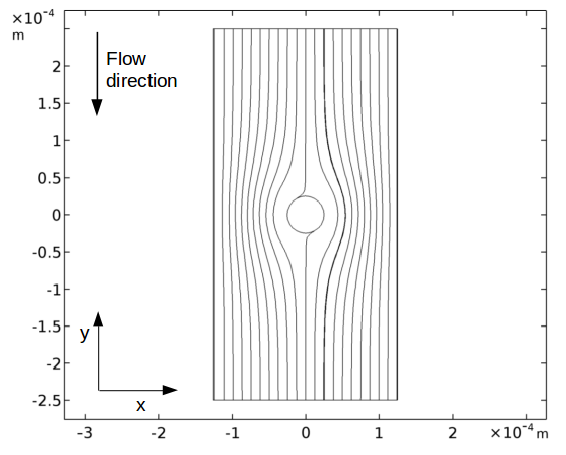
\includegraphics{figures/model_creeping_flow_single_wire.png}}
\caption[Simulated Stokes flow around cylinder]{Simulated streamlines of a creeping flow around a single wire with a velocity of $u_{0}$=20\,mm/s 
\label{fig:creep_flow_sw}
}
\end{figure}

\subsection{Parameter studies}
\label{subsec:Param_res}

Parameter studies were performed to get a better understanding of the influence of the different parameters on the retention behaviour of the nanoparticles.
Most parameter runs were performed with a particle radius of 30\,\textmu m, which fits the volumetric median diameter D50 of 31,25\,\textmu m of the TruForm matrix material used for the retention experiments (see Section\,\ref{subsec:mat_mag_char_res}). In addition to the single wire setup the parameter studies were performed with two and four wire configurations. The resulting magnetic field and flux around the single wire were already described in Section\,\ref{subsec:mod_val}. In the following a short overview of the resulting magentic field and flux around the two and four cylinder setup is given. \\
In Figure\,\ref{fig:tw_fw_mag_field} the simulated magnetic field intensity and the magnetic field lines for two and four magnetized cylindrical wires are shown. It is apparent that the minimum and maximum values of the magnetic field intensity can still be located in the same positions as for a single wire. The highest values for the field strength however decrease from 3.07$\cdotp$10\textsuperscript{-4}\,A/m for the single wire configuration to 2.82$\cdotp$10\textsuperscript{-4}\,A/m and 2.04$\cdotp$10\textsuperscript{-4}\,A/m for the two and four wire setup respectively. As there are more surfaces for the particles to be attracted to than in the single wire setup and the particles can not as easily bypass the wire without being influenced by the magnetic field gradient the retention is assumed to increase with an increase in the number of wires.  

\begin{figure}[H]
		%\centering
            \begin{subfigure}{0.49\textwidth}
                  \flushleft
                  \scalebox{0.36}{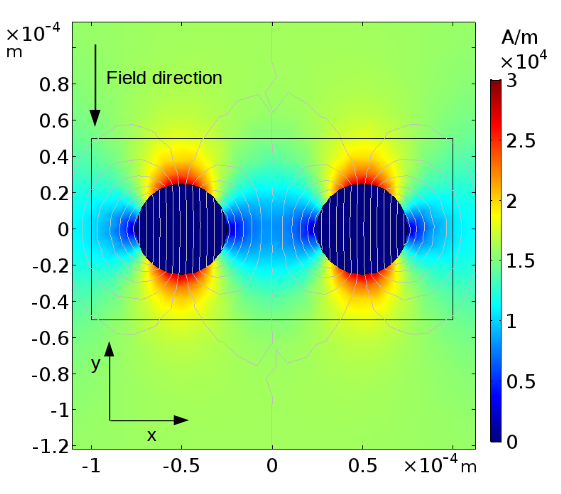
\includegraphics{figures/Hfield_around_two_wires_close.png}}
                  %\caption{}
          \end{subfigure}\hfill
        \begin{subfigure}{0.49\textwidth}
                \flushright
                \scalebox{0.36}{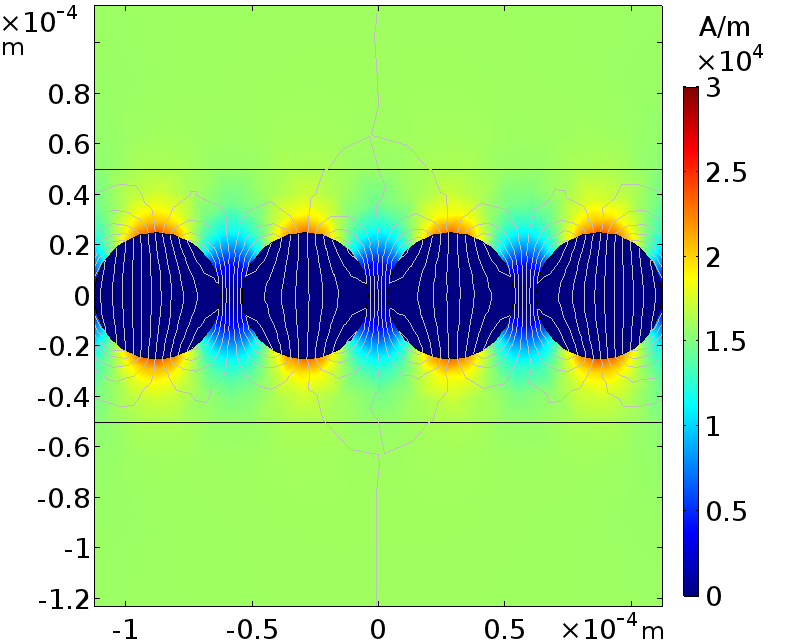
\includegraphics{figures/Hfield_around_four_wires_close.png}}
                %\caption{}\label{fig:creep_2}
        \end{subfigure}
        \\
        
        \caption[Simulated magnetic field intensity around two and four wires]{Simulated magnetic field intensity in A/m and magnetic field lines around two and four ferromagnetic wires for an external magnetic field of 20\,mT \textbf{add figures with larger font}}
        \label{fig:tw_fw_mag_field}
  \end{figure}

In Figure \ref{fig:tw_fw_flow_field} the fluid flow around the two and four wire configuration for $U_{0}$=20mm/s is shown. The no-slip boundary condition on the wire surface leads to a velocity of zero directly at the surface and a forming of a boundary layer in the vicinity. As the cross section between the cylinders is decreased the velocity of the fluid is increased in accordance with Bernoulli's principle. For two cylinders a maximum velocity of 443\,\textmu m/s and for four cylinders of 1640\,\textmu m/s is reached in between the wires, while only a maximum velocity of 310\,\textmu m/s can be observed in the one wire setup. This results in a higher drag force on particles close to the wires.   
  
\begin{figure}[H]
		%\centering
            \begin{subfigure}{0.49\textwidth}
                  \flushleft
                  \scalebox{0.36}{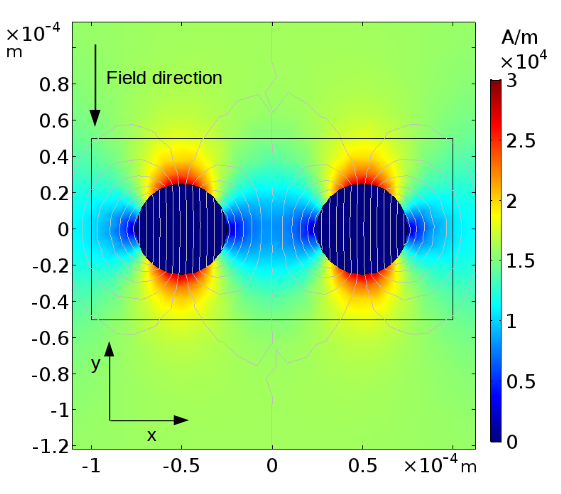
\includegraphics{figures/Hfield_around_two_wires_close.png}}
                  %\caption{}
          \end{subfigure}\hfill
        \begin{subfigure}{0.49\textwidth}
                \flushright
                \scalebox{0.36}{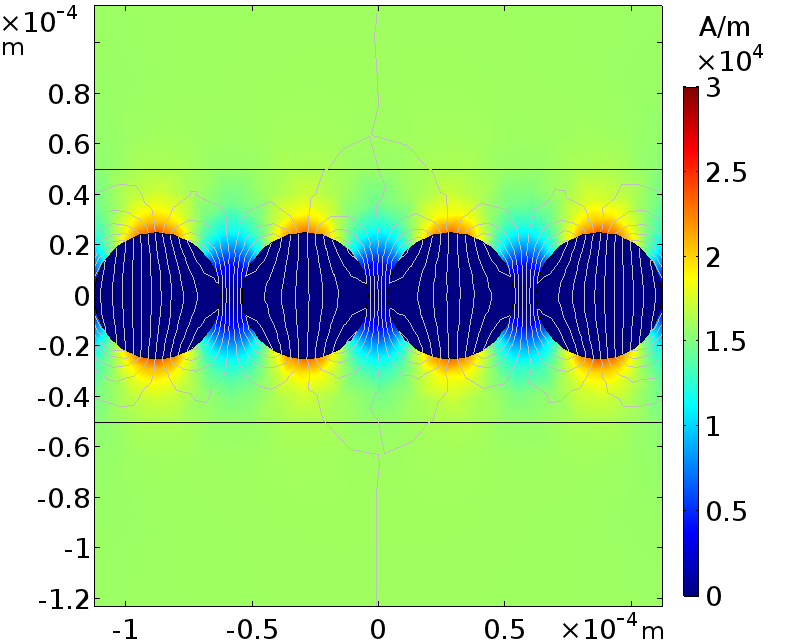
\includegraphics{figures/Hfield_around_four_wires_close.png}}
                %\caption{}\label{fig:creep_2}
        \end{subfigure}
        \\
        
        \caption[]{\textbf{add Figure of streamlines around 2 and 4 cylinders}}
        \label{fig:tw_fw_flow_field}
  \end{figure}  

The results of the parameter studies for the one, two and four wire configurations are presented and discussed in the following Sections (\ref{subsubsec:One_wire}, \ref{subsubsec:Two_wires} and \ref{subsubsec:Four_wires}). 

% A decrease in diameter of the matrix
% element can increase the magnetic field gradient without changing
% the relative distribution of the magnetic field. After reaching the
% magnetic saturation, the magnetic field intensity around the
% matrix with high saturation magnetization, is larger than that of
% the matrix with low saturation magnetization. However, the mag-
% netic field gradient doesn’t change significantly with the increase
% in background induction [31]. This suggests that increasing the
% magnetic field intensity blindly may not necessarily improve the
% separation performance in practical use \cite{ge2017magnetic}
% 
% However, in practical applications, the
% magnetic matrix usually contains a group of elements, and the
% study of a single element may not reflect the real situation of the
% actual matrix. More researches on the magnetic field distribution
% of the matrix in the form of a group of element are required\cite{ge2017magnetic}

% Because particles deposit preferentially on the upstream wires as shown
% in Section III, the wire matrix preferentially becomes saturated with particles
% in the upstream part and increases the pressure drop before all of the wires are
% saturated with particles. Figure 12 suggests that the capture ratio or deposition
% on each wire can be controlled by specifying a combination of the magnetic
% field and fluid velocity for a given capture ratio of the magnetic filt

% Es zeigt sich, dass bei kleineren Achsenabständen der Gitter die Stromlinien bei gleichem
% Ausgangspunkt näher am Draht verlaufen. Hierdurch werden die Partikel näher an den Draht und
% damit in den Bereich größerer Magnetkräfte transportiert, woraus höhere Einfangradien resultiere Aber verstopfung!

\subsubsection{One Cylinder}
\label{subsubsec:One_wire}

\textbf{possibly add different Geometry results}

\textbf{1 Cylinder const speed BC}
\begin{figure}[H]
		%\centering
            \begin{subfigure}{0.49\textwidth}
                  \flushleft
                  \scalebox{0.42}{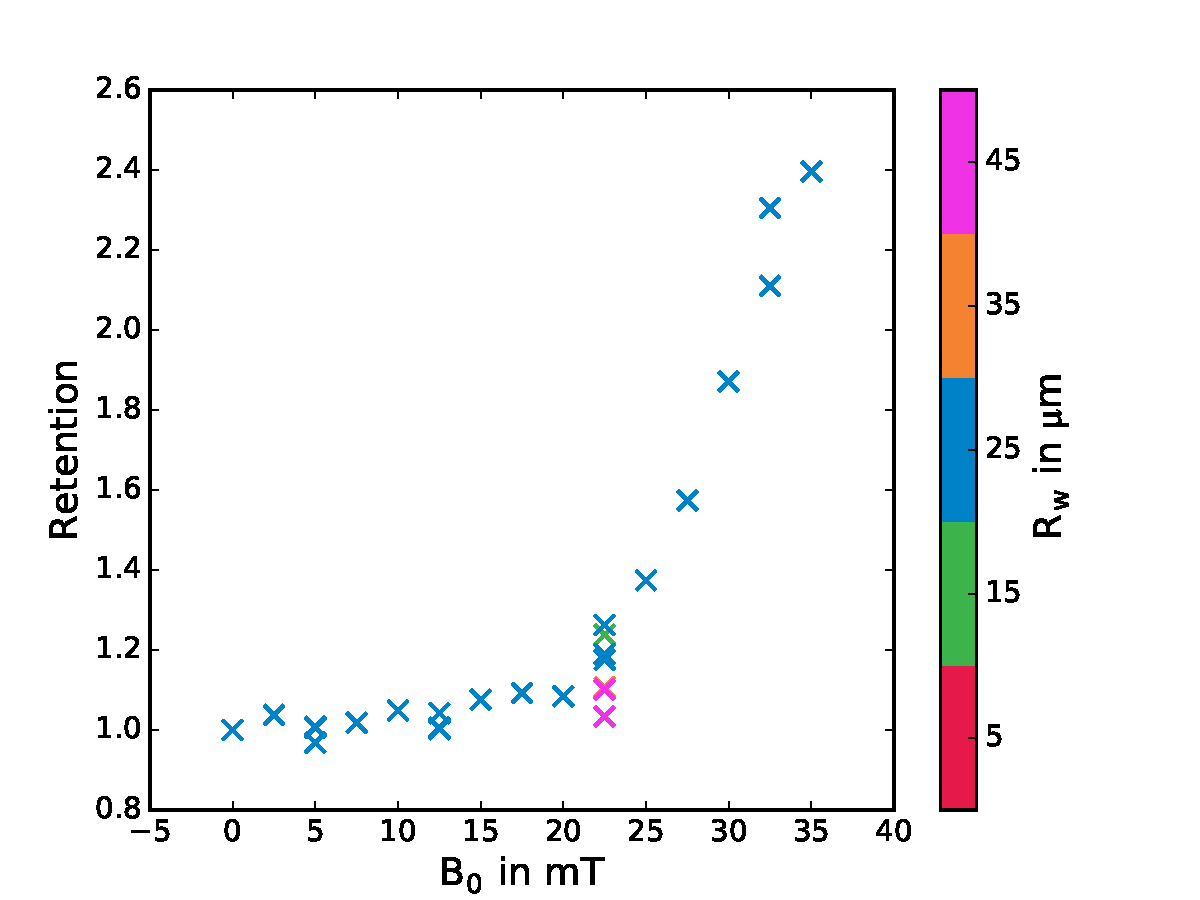
\includegraphics{figures/B0_Rp_30_U0_20_Rw_var_1Cylinder_constBC.pdf}}
                  %\caption{}
          \end{subfigure}\hfill
          \\
            \begin{subfigure}{0.49\textwidth}
                  \flushleft
                  \scalebox{0.42}{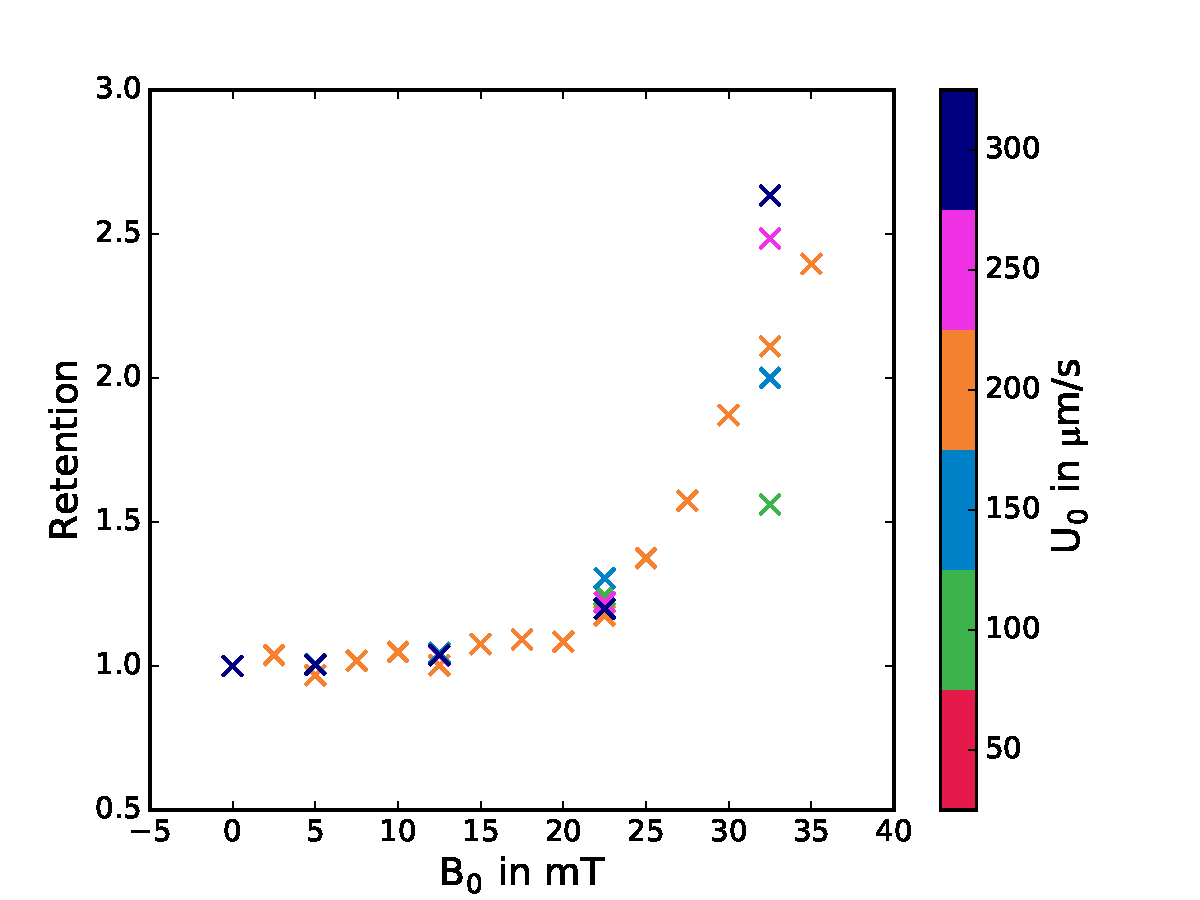
\includegraphics{figures/B0_Rp_30_U0_var_Rw_25_1Cylinder_constBC.pdf}}
                  %\caption{}
          \end{subfigure}\hfill
        \begin{subfigure}{0.49\textwidth}
                \flushright
                \scalebox{0.42}{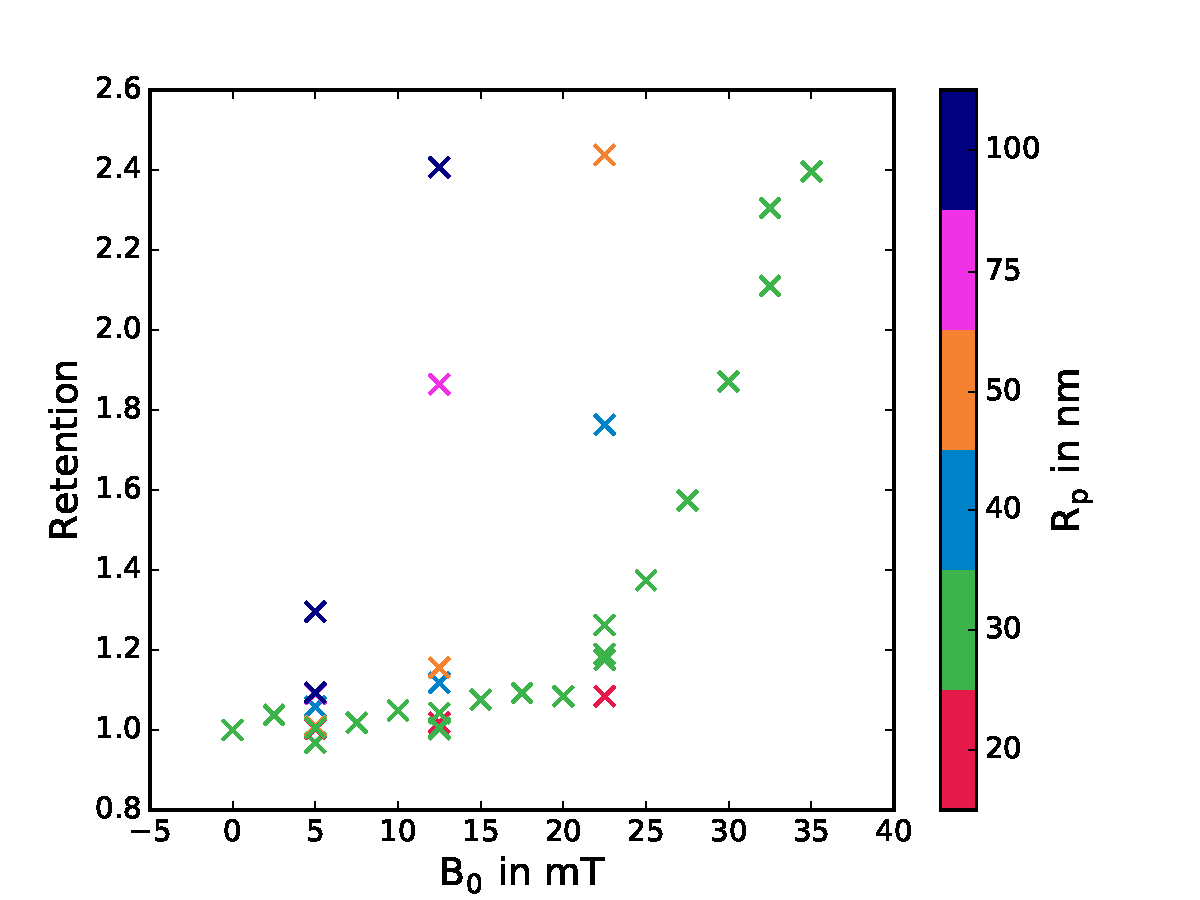
\includegraphics{figures/B0_Rp_var_U0_20_Rw_25_1Cylinder_constBC.pdf}}
                %\caption{}\label{fig:creep_2}
        \end{subfigure}
        \\
        
        \caption[]{}
        \label{fig:tw_fw_mag_field}
  \end{figure}

\textbf{1 Cylinder periodic BC}
\begin{figure}[H]
		%\centering
            \begin{subfigure}{0.49\textwidth}
                  \flushleft
                  \scalebox{0.42}{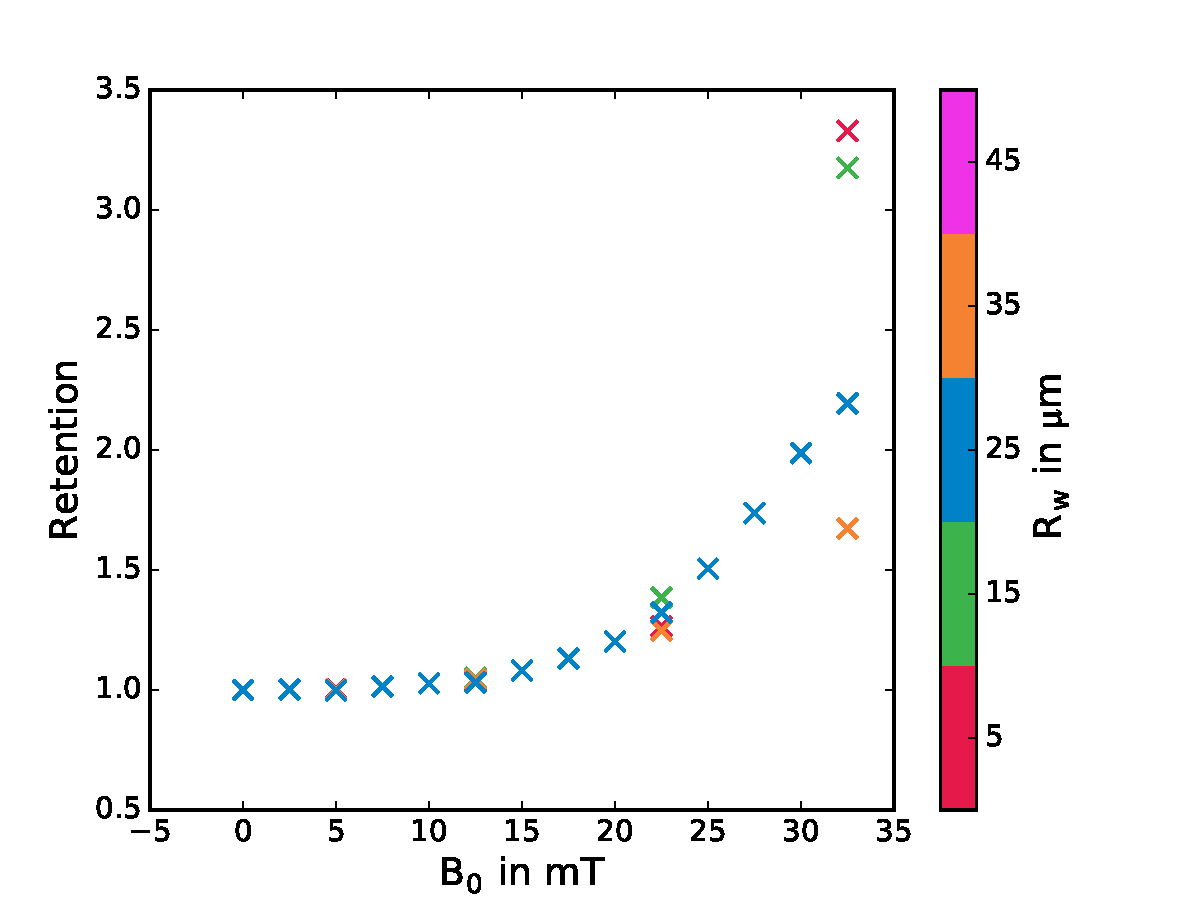
\includegraphics{figures/B0_Rp_30_U0_20_Rw_var_1Cylinder_periodicBC.pdf}}
                  %\caption{}
          \end{subfigure}\hfill
          \\
            \begin{subfigure}{0.49\textwidth}
                  \flushleft
                  \scalebox{0.42}{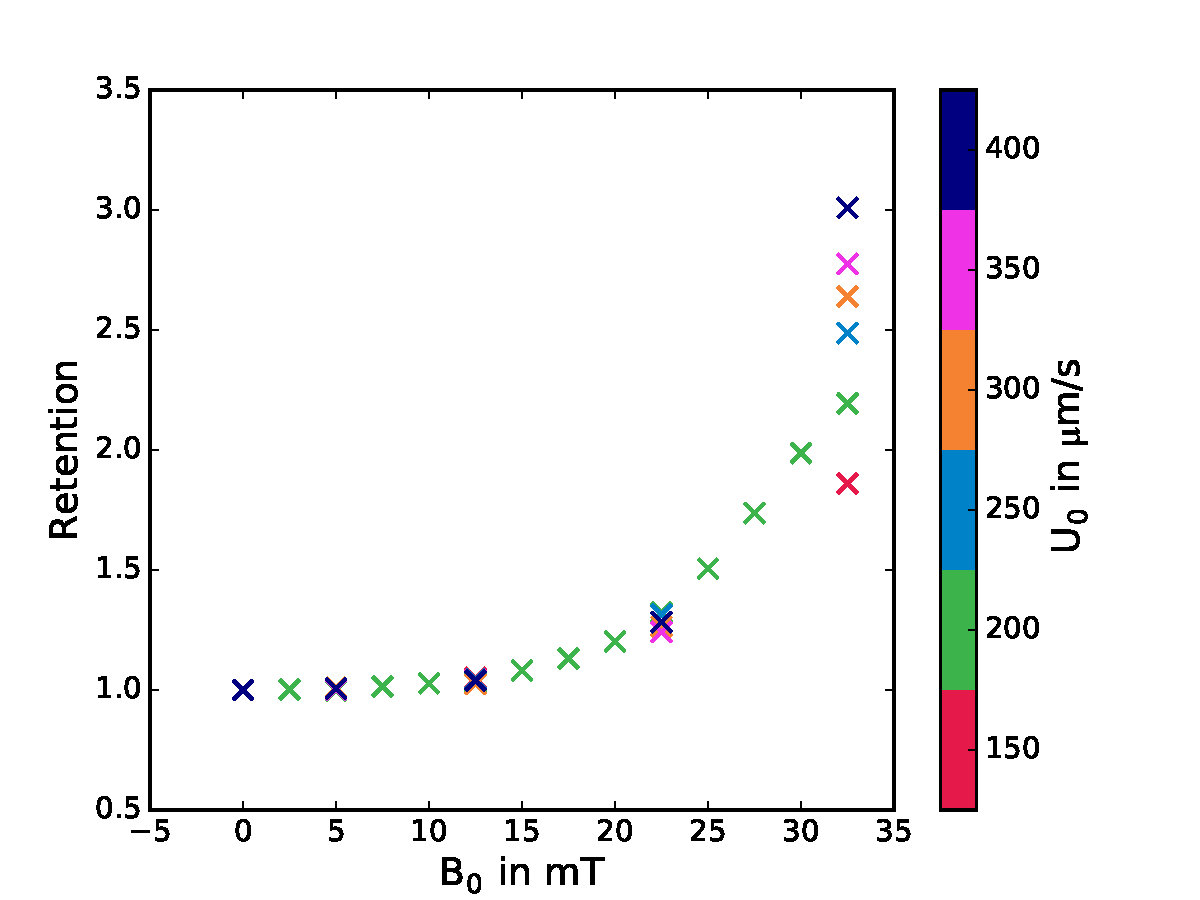
\includegraphics{figures/B0_Rp_30_U0_var_Rw_25_1Cylinder_periodicBC.pdf}}
                  %\caption{}
          \end{subfigure}\hfill
        \begin{subfigure}{0.49\textwidth}
                \flushright
                \scalebox{0.42}{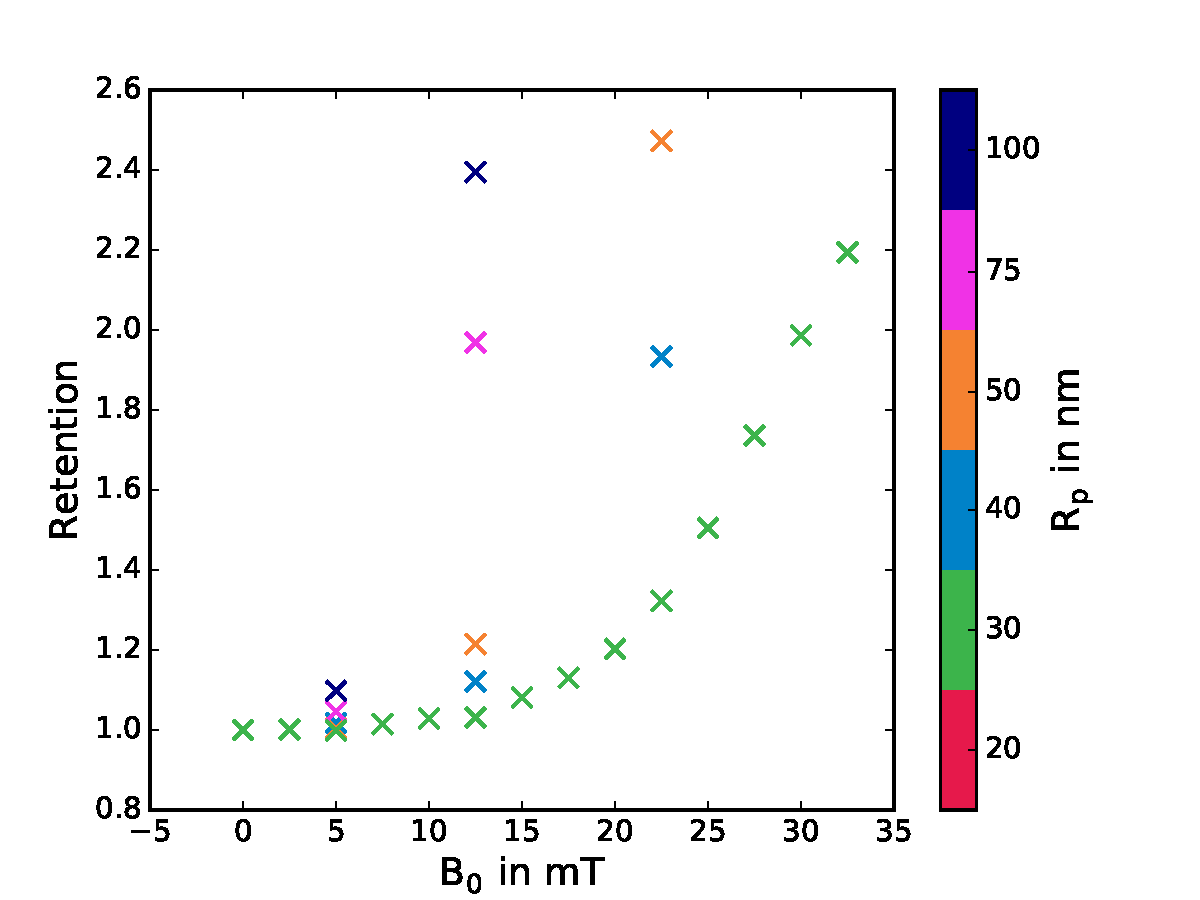
\includegraphics{figures/B0_Rp_var_U0_20_Rw_25_1Cylinder_periodicBC.pdf}}
                %\caption{}\label{fig:creep_2}
        \end{subfigure}
        \\
        
        \caption[]{}
        \label{fig:tw_fw_mag_field}
  \end{figure}


\subsubsection{Two Cylinders}
\label{subsubsec:Two_wires}

\textbf{2 Cylinder const speed BC}
\begin{figure}[H]
		%\centering
            \begin{subfigure}{0.49\textwidth}
                  \flushleft
                  \scalebox{0.42}{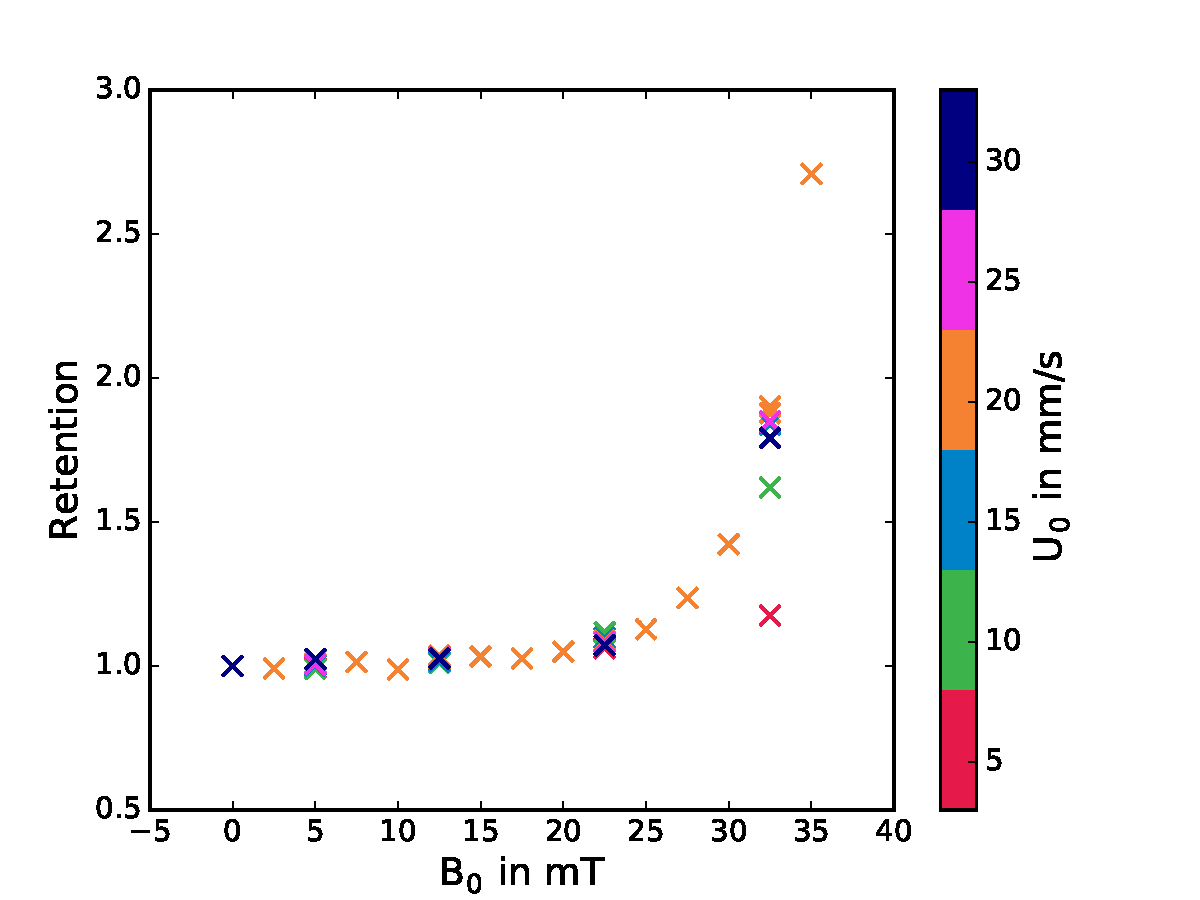
\includegraphics{figures/B0_Rp_30_U0_var_2Cylinder_constBC.pdf}}
                  %\caption{}
          \end{subfigure}\hfill
        \begin{subfigure}{0.49\textwidth}
                \flushright
                \scalebox{0.42}{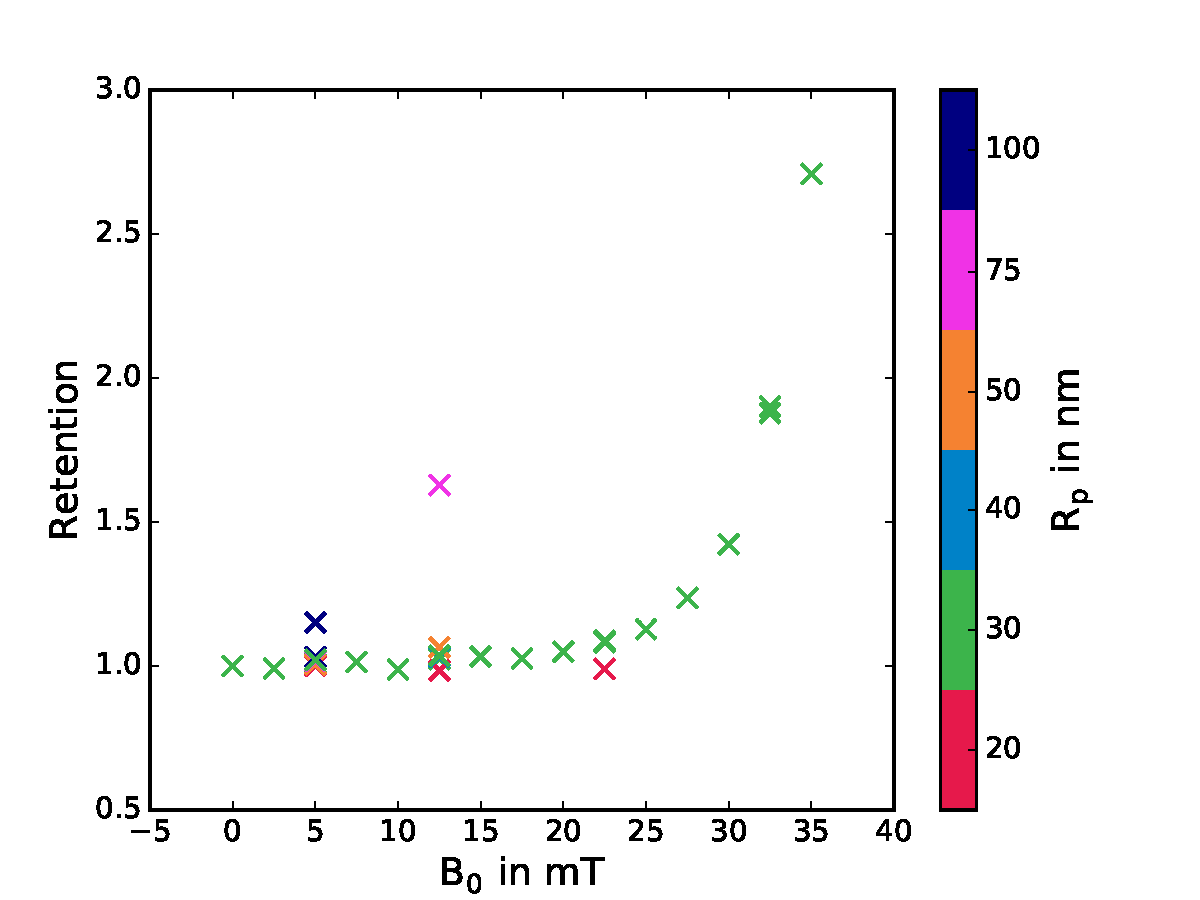
\includegraphics{figures/B0_Rp_var_U0_20_2Cylinder_constBC.pdf}}
                %\caption{}\label{fig:creep_2}
        \end{subfigure}
        \\
        
        \caption[]{}
        \label{fig:tw_fw_mag_field}
  \end{figure}

\textbf{2 Cylinder periodic BC}
\begin{figure}[H]
		%\centering
            \begin{subfigure}{0.49\textwidth}
                  \flushleft
                  \scalebox{0.42}{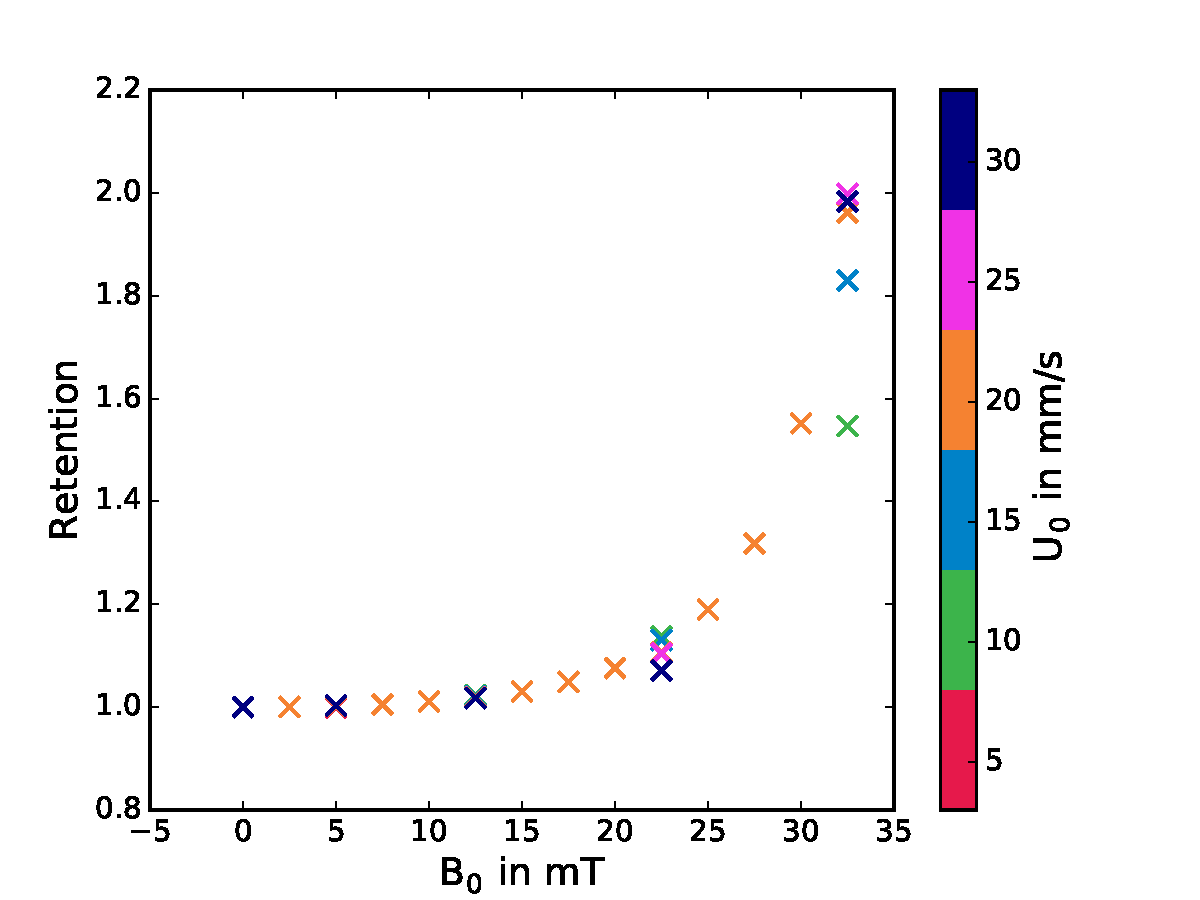
\includegraphics{figures/B0_Rp_30_U0_var_2Cylinder_preiodicBC.pdf}}
                  %\caption{}
          \end{subfigure}\hfill
        \begin{subfigure}{0.49\textwidth}
                \flushright
                \scalebox{0.42}{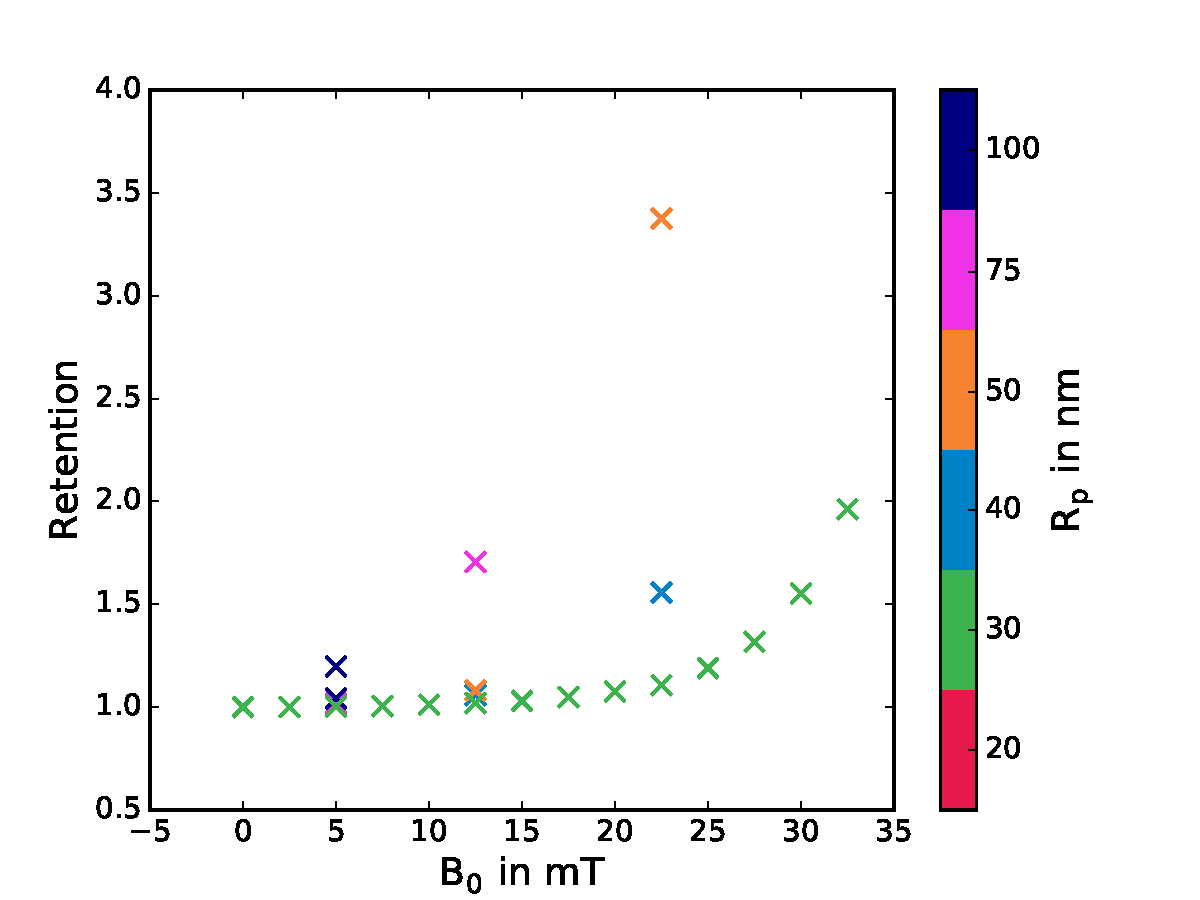
\includegraphics{figures/B0_Rp_var_U0_20_2Cylinder_periodicBC.pdf}}
                %\caption{}\label{fig:creep_2}
        \end{subfigure}
        \\
        
        \caption[]{}
        \label{fig:tw_fw_mag_field}
  \end{figure}

\subsubsection{Four Cylinders}
\label{subsubsec:Four_wires}

\textbf{4 Cylinder const speed BC}
\begin{figure}[H]
		%\centering
            \begin{subfigure}{0.49\textwidth}
                  \flushleft
                  \scalebox{0.42}{\includegraphics{figures/B0_Rp_30_U0_var_4Cylinder_constBC.pdf}}
                  %\caption{}
          \end{subfigure}\hfill
        \begin{subfigure}{0.49\textwidth}
                \flushright
                \scalebox{0.42}{\includegraphics{figures/B0_Rp_var_U0_20_4Cylinder_constBC.pdf}}
                %\caption{}\label{fig:creep_2}
        \end{subfigure}
        \\
        
        \caption[]{}
        \label{fig:tw_fw_mag_field}
  \end{figure}

\textbf{4 Cylinder periodic BC}
\begin{figure}[H]
		%\centering
            \begin{subfigure}{0.49\textwidth}
                  \flushleft
                  \scalebox{0.42}{\includegraphics{figures/B0_Rp_30_U0_var_4Cylinder_periodicBC.pdf}}
                  %\caption{}
          \end{subfigure}\hfill
        \begin{subfigure}{0.49\textwidth}
                \flushright
                \scalebox{0.42}{\includegraphics{figures/B0_Rp_var_U0_20_4Cylinder_periodicBC.pdf}}
                %\caption{}\label{fig:creep_2}
        \end{subfigure}
        \\
        
        \caption[]{}
        \label{fig:tw_fw_mag_field}
  \end{figure}  
  
\section{Experimental results}
\label{sec:exp_res}

\subsection{Matrix material and magnetic nanoparticle characterization}
\label{subsec:mat_mag_char_res}
%PGV, ESEM, Microscope of PMMA, LSM, TruForm, cheamgen, micromod
%magnetic properties(hysteresis loop)

As the material properties, e.g. size, shape and magnetization behaviour, of both the matrix material and the magnetic nanoparticles have a significant influence on the retention behaviour and the separation efficiency the used materials were thoroughly/extensively? tested and characterized. \newline
The volume based particle size distributions for the examined matrix materials are shown in Figure\,\ref{fig:Hist_mat}. The corresponding D-values that were derived from a fit of the cumulative distribution Q$_{3}$ can be found in Table\,\ref{table:D_values_matrix}. 

\begin{table}[h]
\centering
\caption[Volumetric D-values for the matrix material]{Volumetric D-values for the matrix material}
\label{table:D_values_matrix}
\begin{tabularx}{\textwidth}{XXXX}\hline
material specification & D10  & D50 & D90  \\
\hline\hline
TruForm & 16.38\,\textmu m & 31.25\,\textmu m & 47.01\,\textmu m \\
LSM & 24.7\,\textmu m & 46.11\,\textmu m & 81.05\,\textmu m \\
SRA-150 & 8.5\,\textmu m & 18.46\,\textmu m & 34.22\,\textmu m \\
SRA-150 sieved & 8.65\,\textmu m & 18.01\,\textmu m & 32.44\,\textmu m \\
\hline
\end{tabularx}
\end{table} 

It can be seen that the LSM matrix material with a D10 value of 24.7\,\textmu m and a D90 value of 81.05\,\textmu m exhibits a much wider particle size distribution than the two other matrix materials SRA-150 and Truform with D10 values of  8.5\,\textmu m and 16.38\,\textmu m and D90 values of 34.22\,\textmu m and 47.01\,\textmu m respectively. It is desirable for the size of the matrix material particles to be relatively homogeneous, at best varying no more than 10\,\% from the average particle size, in order to achieve a homogeneous packed bed which in turn leads to uniform fluid flow characteristics within the column \cite{miltenyi1997magnetic}. In addition smaller particles produce higher magnetic field gradients and are therefore more suitable for the separation of weakly magnetic materials. Consequently the LSM particles were not further investigated. The remaining matrix materials SRA-150 and TruForm exhibit narrower particle size distributions. With an average particle size of 20.0\,\textmu m and  31.72\,\textmu m and corresponding standard deviations of 11.76\,\textmu m and 9.67\,\textmu m respectively, they vary however further than the above mentioned 10\,\% from the average particle size. The D-values of the TruForm particles show only very slight deviations between 2 to 5\,\% from the manufacturers specifications. for the D50 value  a  In order to decrease the width of the particle size distribution the SRA-150 particles, which were already used in preceiding experiments by \cite{AndreMaster}, were sieved as described in Section\,\ref{subsec:Matrix_mat}. The resulting particle distribution is shown in Figure\,\ref{fig:hist_SRA_sieve}. With an increase of the D10 value by 1.8\,\% and a decrease of the D50 and D90 value by 2.5\,\% and 5.5\,\%  respectively the width of the particle size distribution could not be reduced significantly. This lack of size separation may be due to the dry sieving process applied. For particles smaller than approximately 30\,\textmu m a wet sieving process reduces blocking of the sieve meshes and therefore increase the separation efficiency \cite{RetschSieve}. Nevertheless both the SRA-150 and the TruFrom matrix material were further investigated. 

\begin{figure}[h]
		%\centering
          \begin{subfigure}{0.49\textwidth}
                  %\flushleft
                  \scalebox{0.37}{\includegraphics{figures/Praxair_PGV.pdf}}
                  \caption{TruForm matrix material}\label{fig:hist_TruForm}
          \end{subfigure}\hfill	
	  \begin{subfigure}{0.49\textwidth}
                  %\flushleft
                  \scalebox{0.37}{\includegraphics{figures/LSM_PGV.pdf}}
                  \caption{ LSM matrix material}\label{fig:hist_LSM}
          \end{subfigure}\hfill	\\
          \begin{subfigure}{0.49\textwidth}
                  %\flushright
                  \scalebox{0.37}{\includegraphics{figures/Starck_PGV_Andre.pdf}}
                  \caption{SRA-150 matrix material}\label{fig:hist_SRA}
          \end{subfigure}\hfill
        \begin{subfigure}{0.49\textwidth}
                %\flushright
                \scalebox{0.37}{\includegraphics{figures/Starck_PGV_sieved.pdf}}
                \caption{SRA-150 matrix material sieved}\label{fig:hist_SRA_sieve}
        \end{subfigure}
        \\        
        \caption[Particle size distribution of the matrix materials]{Volume based particle size distribution of the matrix materials with a histogram plot of the density distribution q$_{3}$ (grey bins) and the cumulative distribution Q$_{3}$ (black line)}
        \label{fig:Hist_mat}
  \end{figure}
  
In addition to the particle size distribution the particle shape of the remaining matrix materials was analyzed with the help of \gls{esem} images. It can be seen in \cite{AndreMaster}, that the SRA-150 matrix material consists of particles with partly large deviations form the ideal spherical shape. For the TruForm material shown in Figure \ref{fig:esem_prax} more spherical particles with a much lower percentage of deviating particle shapes can be observed. In addition to a homogeneous size of the matrix particles a spherical shape is required to achieve a uniform spacing between the particles in the separation column \cite{miltenyi1997magnetic}. Uniform magnetic field gradients are generated within the gaps between the spheres and a substantially uniform fluid flow is produced. This configuration is desirable in order to produce a steady and reproducible separation and retention of the nanoparticles. Therefore the TruForm matrix material was choose for the separation experiments.          

\begin{figure}[H]
		%\centering
            \begin{subfigure}{0.49\textwidth}
                  \flushleft
                  \scalebox{0.15}{\includegraphics{figures/310118TruForm316-3Praxair(MP1).png}}
                  %\caption{}
          \end{subfigure}\hfill
        \begin{subfigure}{0.49\textwidth}
                \flushright
                \scalebox{0.15}{\includegraphics{figures/310118TruForm316-3Praxair(MP1-2).png}}
                %\caption{}\label{fig:creep_2}
        \end{subfigure}
        \\
        
        \caption[ESEM images of the TruForm matrix material]{TruForm matrix material imaged with the aid of the \gls{esem} in two different resolutions}
        \label{fig:esem_prax}
  \end{figure}

In order to verify the suitability of the TruForm material for the use as separation matrix the magnetic properties of the particles were determined with an \gls{agm} described in Section\,\ref{subsubsec:Mag_char}. Due to the composition of the Truform material with high percentages of iron and chromium (see Table\,\ref{table:mat_material}) ferromagnetic behaviour with a low remanence was expected. The resulting magnetization curve is shown in Figure\,\ref{fig:Prax_hyst}. As expected the TruForm material exhibits ferromagnetic behaviour, which can be seen by the displayed hysteresis loop. From this hysteresis loop the magnetic properties of the material can be extracted (see Section \ref{subsec:Mag_mat}). The suitability of a material for magentic separation can be determined by its coercivity $H_{c}$ and its ratio of the remanence to saturation magnetization $M_{R}/M_{S}$. Magnetically soft materials with a value of $H_{c}$ below 1\,kA/m are desirable as matrix materials, as they are easily magnetized and more importantly retain almost no remanent magentization once the magentic field is removed. This behaviour enables a simple removal of collected nanoparticles from the column after a retention experiment. However the TruForm particles with a $H_{c}$ value of 3.55\,kA/m do retain a remanence magentization. This is also emphasized by the ratio of the remanence to the saturation magnetization which is with 3.85\,\% much larger than the 1\,\% or less that is necessary to resuspend the particles completely after the magentic field is turned of. Therefore the column packed with the TruForm matrix material was demagnetized to remove all collected nanoparticles after each experimental cycle and to restore the initial conditions.\\ 

\begin{figure}[h]
\centering

\scalebox{0.5}{\includegraphics{figures/Prax_hyst.pdf}}
\caption[Magnetization curve of the TruForm matrix material]{Magnetization curve of the TruForm matrix material: the magentization M is plottet against the magnetic field strength H in addition the measured values for the coercivity $H_{c}$, the remanence magnetization $M_{r}$, the saturation magnetization $M_{s}$ and the ratio of the remanence to saturation magnetization $M_{R}/M_{S}$ are displayed
\label{fig:Prax_hyst}
}
\end{figure}

The particle size and shape of the \gls{pmma} matrix material, which was used as a negative control with its non-magnetic behaviour, was determined under the light microscope. The diameter of the spherical particles was measured with the distance measurement function of the light microscope as described in Section\,\ref{subsubsec:light_mic}. An exemplary microscope image of the \gls{pmma} particles with diameter measurements is shown in Figure\,\ref{fig:PMMA}. It can be clearly seen that the particles are almost perfectly spherical and of a uniform size of approximately 17\,\textmu m, which matches the manufacturers specifications. The uniform spheres, with a variation of less than 5\,\% around the average size of 17\,\textmu m, form a closely stacked lattice within the column, that results in uniform channels for homogeneous fluid flow.

\begin{figure}[h]
\centering

\scalebox{0.2}{\includegraphics{figures/PMMA.pdf}}
\caption[Light microscope image of \gls{pmma}]{Light microscope image of the \gls{pmma} matrix material
\label{fig:PMMA}
}
\end{figure}

The particle size distributions of the magnetic nanoparticle suspensions were measured via dynamic light scattering. In order to evaluate the nanoparticles the D-values were determined by a fit of the cumulative distribution Q$_{3}$. The resulting volume based particle size distributions and the calculated D-values can be found in Figure\,\ref{fig:Hist_nano} and Table\,\ref{table:D_values} respectively.

\begin{table}[h]
\centering
\caption[Volumetric D-values for the magnetic nanoparticles]{Volumetric D-values for the magnetic nanoparticles}
\label{table:D_values}
\begin{tabularx}{\textwidth}{XXXX}\hline
material specification & D10  & D50 & D90  \\
\hline\hline
Chemagen filtrated & 63.17\,nm & 101.06\,nm & 189.59\,nm \\
micromod 100\,nm & 28.41\,nm & 99.96\,nm & 185.65\,nm \\
micromod 20\,nm & 19.23\,nm & 40.67\,nm & 74.70\,nm \\
micromod mixture & 22.16\,nm & 44.17\,nm & 80.39\,nm \\
\hline
\end{tabularx}
\end{table}  

\begin{figure}[h]
		%\centering
          \begin{subfigure}{0.49\textwidth}
                  %\flushleft
                  \scalebox{0.37}{\includegraphics{figures/ChemagenfiltStandard.pdf}}
                  \caption{Chemagen nanoparticles filtrated }\label{fig:hist_chemagen}
          \end{subfigure}\hfill	
	  \begin{subfigure}{0.49\textwidth}
                  %\flushleft
                  \scalebox{0.37}{\includegraphics{figures/hist20180316MF100MixFeed1.pdf}}
                  \caption{micromod particles mixture 1:1}\label{fig:hist_micro_mix}
          \end{subfigure}\hfill	\\
          \begin{subfigure}{0.49\textwidth}
                  %\flushright
                  \scalebox{0.37}{\includegraphics{figures/hist20180316MF100100nmFeed1.pdf}}
                  \caption{micromod particles 100\,nm}\label{fig:hist_micro_100}
          \end{subfigure}\hfill
        \begin{subfigure}{0.49\textwidth}
                %\flushright
                \scalebox{0.37}{\includegraphics{figures/hist20180316MF10020nmFeed1.pdf}}
                \caption{micromod particles 20\,nm}\label{fig:hist_micro_20}
        \end{subfigure}
        \\        
        \caption[Volumetric particle size distribution of the magnetic nanoparticles]{Particle size distribution of the magnetic nanoparticles with the density distribution q$_{3}$ (dotted black line) with error bars, the cumulative distribution Q$_{3}$ (black line) and the fit of Q$_{3}$ (dotted red line) for the calculation of the D-values}
        \label{fig:Hist_nano}
  \end{figure} 

It was already demonstrated by \cite{AndreMaster}, that the Chemagen nanoparticles form aggregates. Therefore the nanoparticles were filtered through a filter with a pore size of 450\,\textmu m before each experiment to remove the largest aggregates from the particle suspension, which should minimize a size exclusion effect within the column. In Figure\,\ref{fig:hist_chemagen} it can be clearly seen that no particles larger than the filter pore size were detected in the filtered solution. With a volumetric D50 value of 101.06\,\textmu m the Chemagen nanoparticles still considerably larger than the average particle size of 10\,nm to 20\,nm in magnetic nanoparticle suspensions mentioned by \cite{svoboda2004magnetic}. In addition a wide particle size distribution from approximately 50\,nm to 400\,nm is apparent. This can also be attributed to the agglomeration of the particles with an individual size between 20\,nm and 50\,nm.
In order to get a more precise evaluation of the separation efficiency of the tested column nanoparticles with a more narrower particle size distribution from micromod were examined. The results of the particle size measurements of the micromod particles for two different particle sizes, 20\,nm and 100\,nm, as well as a 1:1 mixture of the two suspensions are also depicted in Figure\,\ref{fig:Hist_nano}. It can be clearly seen that all three solutions exhibit far narrower particle size distributions in a range between approximately 20\,nm to 300\,nm. The measured volumetric D50 value of 99.96\,nm fits very well with the manufacturers data of an average particle size of 100\,nm. For the 20\,nm particles however the determined D-value of 40.67\,nm is much larger than the indicated 20\,nm range. The variation could however also result from the volumetric approach of the particle measurement in which larger particles have a stronger influence on the D-values than in an number based approach. For the 20\,nm micromod particles a bimodal distribution is observed. The first mode exhibits a mean particle size of approximately 20\,nm, while the second mode is comparable to the size distribution of the 100\,nm particles. Aggregation of the nanoparticles is unlikely as the unmodified dextran surface is negatively charged, which leads to mututal repulsion of the particles. In addition 20\,nm is close to the sensitivity limit of most measurement systems and it is very difficult to produce uniform particles in that size range. According to the manufacturer specifications a deviation of the particle size of up to 100\,nm can be possible for the 20\,nm particles. The mixture of the two particle sizes, which was used for separation experiments, also results in a bimodal size distribution which is shown in Figure \ref{fig:hist_micro_20}. A first mode at approximately 20\,nm and a second mode at around 50\,nm can be observed. Despite the deviations of the particle  size the micromod particles exhibit a much smaller particle size distribution than the Chemagen nanoparticles, which makes them more suitable for initial separation experiments. According to manufacturers specifications the size of the magnetite domains within the micromod particles lies between 5 and 15\,nm. As this is a much smaller domain size than the critical size for magetite of 0.05\,\textmu m, the micromod nanoparticles are superparamagnetic. In \cite{AndreMaster} it was also shown that the Chemagen nanoparticles exhibit superparamagnetic behaviour. 

% a high magnetic field gradient is locally induced close to the surface of the matrix
% 
% spheres form a closely stacked lattice, which creates substantially uniform channels for homogeneous flow during separations. homogeneous flow characteristics
% 
% uniform magnetic field gradients and flow characteristics
% 
% It is desirable that the size of spheres be relatively homogeneous, usually varying not more than about 15% from the average size, more usually by not more than about 10%, and preferably by not more than about 5%.
% The substantially symmetrical spherical shape and substantially uniform size of the spheres are desirable for the construction of a magnetic separator matrix, as the spheres can assume a lattice configuration wherein the gaps between the spheres form regular channels or pores in the matrix.
% Upon the application of a magnetic field to the separator, magnetic field gradients are created in the gaps between the spheres. The uniform size, and therefore spacing, of the spheres provides for a substantially uniform magnetic gradient throughout the matrix, and substantially uniform fluid flow characteristics.


\subsection{Flow rate optimization}
\label{subsec:flow_rate_res}

The two matrix materials \gls{pmma} and TruForm were selected for the retention experiments based on their magnetic porperties, shape and particle size distribution. In a next step the optimal flow rate for the packed column in a \gls{fplc}-system was determined. Three different flow rates, 0.1\,ml/min, 0.2\,ml/min and 0.5\,ml/min, were tested for the two materials with the Chemagen nanoparticles diluted in 20\,mM phosphate buffer. Higher flow rates where not considered due to the high pressure build-up and the pressure limit of the glass column and filters at 80\,bar. Exemplary curves resulting form the different flow rates for the TruForm matrix material are displayed in Figure \ref{fig:flowrate_prax}. The conductivity peak is caused by the 20\,mM phosphate buffer, which is used as tracer as it is not influenced by either the matrix material or the magnetic field and therefore always has a similar shape, area and peak maximum. All three UV-peaks exhibit a baseline width of about 1.85\,ml with a peak maximum at approximately 0.6\,ml. the peak maximum however varies from 230\,mAu for a flow rate of 0.2\,ml/min to 140\,mAu for a flow rate of 0.1\,ml/min. 
For an ideal packed bed the resulting peaks should exhibit a Gaussian profile. Due to inhomogeneities in the packed bed and dead volume in the flow path deviations like fronting and tailing can occur. Tailing can also be observed for all three tested flow rates. As a flow rate of 0.5\,ml/min was already used by \cite{AndreMaster} and a high number of screening experiments was only possible with higher flow rates, a flow rate of 0.5\,ml/min was chosen.         

\begin{figure}[H]
\centering

\scalebox{0.6}{\includegraphics{figures/Comp_Flowrates_Prax.pdf}}
\caption[Comparison of different flow rates for the TruForm matrix material]{Comparison of different flow rates for the TruForm matrix material with the Chemagen nanoparticle suspension on a \gls{fplc}-system: The UV-signal at 280\,nm in mAu and the conductivity in mS/cm are plotted against the volume in ml   
\label{fig:flowrate_prax}
}
\end{figure}

In order to quantify the tailing and to evaluate the quality of the packed bed the asymmetry factor $A_{s}$ was determined as describe in Section \ref{sec:peak_as} for the column with an acetone peak. A value of $A_{s}$ smaller than 1 indicates fronting, while a value of $A_{s}$ larger than 1 indicates tailing. For a packing with \gls{pmma} asymmetry between 1 and 2 and for a packing with the TruForm particles an asymmetry between 1 and 1.5 was considered tolerable. Those values were determined by analysing multi
ple acetone peaks for several newly packed columns for each matrix material. For deviating values of $A_{s}$ the column was repacked. 

% \begin{figure}[H]
% 		\centering
%           \begin{subfigure}{0.49\textwidth}
%                   %\flushleft
%                   \scalebox{0.4}{\includegraphics{figures/0mT_PMMA_chemagen.pdf}}
%                   \caption{\textbf{}}\label{fig:Bioreactor_Geometry}
%           \end{subfigure}
%         \begin{subfigure}{0.49\textwidth}
%                 %\flushright
%                 \scalebox{0.3}{\includegraphics{figures/Praxair_0mT_chemagen.pdf}}
%                 \caption{Chromatographic column within the Helmholtz coil}\label{fig:Bioreactor_cross_section}
%         \end{subfigure}
%         \\
%         
%         \caption{Chromatographic system and the used Helmholtz coil}
%         \label{fig:Rep_peak}
%   \end{figure}  



\subsection{Retention experiments with the PMMA matrix material}
\label{subsec:pmma_res}

As the aggregates in the Chemagen nanaoparticl suspension could not be completely removed by an ultrasonic treatment (see Section \ref{Sec:}) it could not be guaranteed that the solution was comprised of the same amount of particles each experimental cycle. Therefore the results of each cycle were noramlized with experimental runs at 0\,mT with the same sample solution.  


\subsection{Retention experiments with TruForm matrix material}
\label{subsec:trufrom_res}

\subsubsection{Separation experiments with the Chemagen nanoparticles}
\label{subsubsec:chemagen_res}

\subsubsection{Separation experiments with micromod nanoparticles}
\label{subsubsec:micromod_res}